\documentclass[12pt,a4paper]{report}

\usepackage[utf8]{inputenc}
\usepackage[T1]{fontenc}
\usepackage[english]{babel}
\usepackage{caption}
\usepackage{subcaption}

\addto\captionsenglish{\renewcommand{\tablename}{Table}}
\addto\captionsenglish{\renewcommand{\listtablename}{List of Tables}}


\usepackage{graphicx}
\graphicspath{{../assets/images/}}
\usepackage{float}
\usepackage{amsmath, amssymb}
\usepackage{hyperref}
\usepackage{geometry}
\geometry{margin=1in}


\pagenumbering{roman}

\begin{document}

\begin{titlepage}
	\centering
	
\includegraphics[width=0.1\textwidth]{logo_uh}\\[1.5cm]
	{\LARGE \textbf{University of Havana}}\\[0.5cm]
	{\Large Faculty of Physics}\\[2cm]
	{\Huge \textbf{Causal discovery applied to gene deregulation networks}}\\[3cm]
	
	{\Large Author:}\\[0.5cm]
	{\LARGE Frank Eduardo Castel Martín}\\[1.5cm]
	
	{\Large Advisors:}\\[0.5cm]
	{\large Gabriel José Gil Pérez}
	\\
	{\large Augusto de Jesús González García}\\[2.5cm]
	
	{\large Diploma Thesis}\\[0.3cm] submitted in partial fulfillment of the requirements for the degree of\\[0.3cm]
	\textbf{Bachelor of Science in Physics}\\[1.5cm]
	
	{\large June 2025}
\end{titlepage}
\newpage



% ====================
% Summary and Abstract
% ====================
\chapter*{Abstract}
Causal discovery is a key tool for inferring cause-and-effect relationships from observational data, with relevant applications in cancer bioinformatics. This thesis evaluates the performance of a nonparametric causal discovery algorithm implemented in the \texttt{CChains} code, developed to infer gene deregulation networks from gene expression data. The first objective is to validate the method using synthetic data generated from known causal graphs, allowing a quantitative comparison between the inferred and original graphs. Performance metrics such as discovery fraction, structural similarity, and spurious-edge elimination fraction are used to assess the algorithm under various topological configurations. Subsequently, the method is applied to real gene expression data from normal and tumor tissue samples corresponding to prostate adenocarcinoma (PRAD), lung adenocarcinoma (LUAD), and lung squamous cell carcinoma (LUSC), retrieved from the TCGA database. Finally, genes with high structural relevance are identified in the resulting causal networks by applying centrality measures from graph theory. The results validate the proposed method under reasonable probabilistic assumptions and suggest a set of candidate genes potentially involved in cancer-associated gene regulation mechanisms.

\newpage

\tableofcontents
\listoffigures
\listoftables
\newpage


\pagenumbering{arabic}

% ====================
% Introduction
% ====================
\chapter*{Introduction}
\addcontentsline{toc}{chapter}{Introduction}

The discovery of causal relationships has historically been one of the greatest challenges in the natural and social sciences. Unlike the mere identification of statistical correlations, causal discovery involves understanding the underlying dynamics that link variables or events, which enables not only a more accurate prediction of phenomena but also the possibility of intervening on them in a targeted and effective manner\cite{pearl}. In cancer bioinformatics, this capability is critically important: genetic mutations and alterations in gene expression are deeply interconnected, and the deregulation of these molecular processes plays a central role in the development and progression of disease\cite{cascades}. Thus, the need to infer networks of causal relationships, rather than simple associations, is essential for understanding carcinogenesis and proposing new intervention strategies\cite{causcorr}.

Gene deregulation networks provide a structural model for analyzing how changes in the expression of certain genes can trigger cascades of alterations in others, thereby promoting oncogenic processes\cite{cascades}. This work builds on the previous development of a nonparametric causal discovery algorithm, implemented in the \textit{CChains} code\cite{parametric}, designed to infer causal networks from binary matrices representing gene deregulation across different normal and tumor clinical samples. Discovering causal relationships in these networks makes it possible, among other benefits, to identify driver genes whose initial deregulation may act as an engine of malignant transformation. Understanding and mapping these networks not only broadens our basic understanding of cancer biology, but also opens the door to the identification of biomarkers and potential therapeutic targets\cite{biomarkers}. Likewise, this study uses gene expression data obtained from \textit{The Cancer Genome Atlas} (TCGA), one of the most complete and standardized sources of cancer molecular profiles\cite{prad,luad,lusc}.

In this context, the present thesis addresses the problem of how to perform and validate causal discovery from omics data, particularly gene expression data, in complex diseases such as cancer. Although important advances have been made in the inference of coexpression or correlation networks\cite{coexpresion}, significant challenges remain in the direct inference of causal networks from observational data\cite{observacionales}, especially in high-dimensional scenarios with the reduced number of samples that is typical of genomic data\cite{dimentionality}.

This work is organized around the following specific objectives:

\begin{itemize}
    \item To verify the correct operation of the causal discovery algorithm implemented in \textit{CChains} using synthetic data sets in which the underlying causal relationships are known in advance, in order to evaluate the ability of the method to reconstruct true causal networks.
    \item To apply this algorithm to real problems in cancer bioinformatics by analyzing gene expression data from tumor and normal samples for several tissues.
    \item To explore and suggest genes of high importance in the inferred gene deregulation networks, using graph-theory metrics such as degree centrality, betweenness centrality, and other relevant measures.
\end{itemize}

To achieve these objectives, the thesis is structured as follows:

\begin{itemize}
	\item \textbf{Chapter 1:} Basic notions of graph theory with applications to biological networks are provided, emphasizing the use of metrics that make it possible to identify vertices with high structural relevance within a gene network.

    \item \textbf{Chapter 2:} The foundations of causal discovery and the main current approaches for developing it from observational data are briefly addressed. The chapter focuses on the algorithm implemented in the \textit{CChains} code, its operation, and the strategies for its validation with synthetic data.

    \item \textbf{Chapter 3:} The results obtained are presented. First, the validation experiments of the algorithm on synthetic data are discussed by comparing the inferred network with known causal networks. Then, the application of the algorithm to real gene expression data from prostate and lung cancer is presented, and the resulting networks are analyzed in terms of relevant genes and other global properties of interest.

	\item \textbf{Chapter 4:} The conclusions of the research are summarized.    
    
\end{itemize}


\newpage


% ====================
% Chapter 1: Graph Theory and Network Analysis
% ====================
\chapter{Elements of Graph Theory in the Study of Gene Deregulation Networks}

The structural analysis of complex systems through graphs is a fundamental tool in disciplines as diverse as physics, computer science, biology, and the social sciences\cite{grafos1}. In particular, gene deregulation networks can be represented as directed graphs, where vertices correspond to genes and edges represent causal relationships between them\cite{grafos2}. This representation makes it possible to apply formal techniques from graph theory \cite{grafos3} to characterize the architecture of the network and identify key vertices.

\section{Basic concepts}

A directed graph \( G = (V, E) \) is composed of a set of vertices \( V \), which represent entities (for example, genes), and a set of directed edges \( E \subset V \times V \), which model relationships among them. A directed edge (or arc) from \( i \) to \( j \), denoted by \( i \to j \), indicates that \( i \) has a certain relationship with \( j \). If there are no cycles in the graph, $G$ is said to be a directed acyclic graph (DAG).

Some relevant concepts are defined below:

\begin{itemize}
    \item \textbf{Parent:} A vertex \( i \) is a parent of \( j \) if there is an edge \( i \to j \) in $G$ (that is, if \( i \to j \in E \)).
    \item \textbf{Child:} Conversely, \( j \) is a child of \( i \) if \( i \to j \in E \).
    \item \textbf{Orphan vertex:} A vertex is orphan if it has no parents in the graph.
    \item \textbf{Terminal vertex:} A vertex is terminal if it has no children in the graph.
     \item \textbf{Path:} A sequence of edges that connects a sequence of vertices.
     \item \textbf{Directed path:} An ordered sequence of vertices \( v_1, v_2, \dots, v_k \) such that, for each consecutive pair \( (v_i, v_{i+1}) \), there exists a directed edge \( v_i \to v_{i+1} \) in the graph.
    \item \textbf{Ancestor:} A vertex \( i \) is an ancestor of \( j \) if there is a directed path from \( i \) to \( j \).
    \item \textbf{Descendant:} Vertex \( j \) is a descendant of \( i \) if \( i \) is its ancestor.
    \item \textbf{Cycle:} A directed path that begins and ends at the same vertex.
    \item \textbf{Transitive edge:} An edge \(i \to j \) is transitive if there exists a directed path from \( i \) to \( j \) that passes through at least one intermediate vertex. In the context of causal discovery, additional requirements are imposed on transitive edges: the directed path must be formed by edges that represent direct (non-spurious) causal relationships, and the edge \(i \to j \) cannot itself represent a direct causal relationship.
    \item \textbf{Set of transitive edges} \( E_t(G) \): Given a directed graph \( G \), \( E_t(G) \) is defined as the set of all transitive edges existing in \( G \). Its cardinality, denoted by \( |E_t(G)| \), represents the total number of such edges.
    \item \textbf{Set of double edges} \( E_d(G) \): This is defined as the set of pairs of vertices \( \{i, j\} \) such that both \( i \to j \) and \( j \to i \) exist in the graph \( G \). The total number of these pairs is denoted by \( |E_d(G)| \) and represents the number of bidirectional relationships present in the network. 
\end{itemize}

These notions make it possible to define hierarchical relationships within the network and are fundamental for causal analysis.

\section{Computational representation of graphs}
	
For the computational treatment of graphs, it is necessary to define structures that efficiently represent the relationships between vertices. The two most widely used representations are the adjacency matrix and the adjacency list.

\textbf{Adjacency matrix:} This is a square matrix A of size n $\times$ n, where n is the number of vertices in the graph. The element $A_{ij}$ takes the value 1 if there is a directed edge from vertex i to vertex j, and 0 otherwise. This representation allows fast access to the existence of direct connections between pairs of vertices, at the cost of greater memory use, especially for sparse graphs.

\textbf{Adjacency list:} In this representation, each vertex maintains a list of the vertices to which it is connected by outgoing directed edges. It is a more efficient structure for storing graphs with a large number of vertices. The size of each adjacency list corresponds to the out-degree of the corresponding vertex, unlike the adjacency matrix, where the size of each list corresponds to the order of the graph.

\textbf{Graph transposition:} Given a directed graph $G=(V,E)$, its transposed graph $G^{T}$ is defined as the graph in which the direction of all edges of G is reversed. Formally, if i $\rightarrow$ j $\in$ E, then $G^{T}$ includes j $\rightarrow$ i. In terms of adjacency matrices, this is equivalent to matrix transposition: $A^{T}_{ij}$ = $A_{ji}$. This operation makes it possible, for example, to identify the parents of a given vertex from its children in the transposed graph.\\

These representations are fundamental for graph storage and analysis, as well as useful tools for facilitating the extraction of global, local, and comparative metrics among graphs. 

\noindent
Figure~\ref{fig:grafo_simple} illustrates a concrete example of a simple directed graph with five vertices numbered from 1 to 5. The connections between vertices are represented by edges that indicate the direction of the relationships. From this graph, its adjacency matrix is constructed (Figure~\ref{fig:matriz_adyacencia}) and the adjacency list associated with vertex 1 is shown (Figure~\ref{fig:lista_adyacencia}).\\

\begin{figure}[h!]
\centering
\begin{subfigure}[b]{0.25\textwidth}
	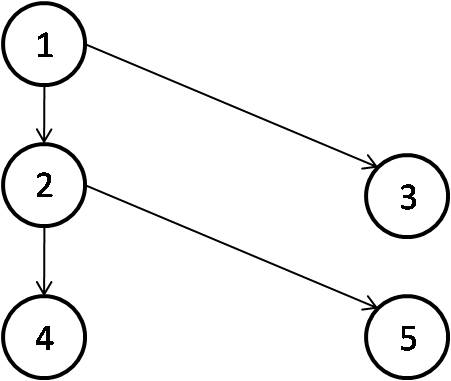
\includegraphics[width=\textwidth]{im.jpg}
	\caption{}
	\label{fig:grafo_simple}
	\end{subfigure}
	\hfill
\begin{subfigure}[b]{0.3\textwidth}
\[
\begin{bmatrix}
0 & 1 & 1 & 0 & 0 \\
0 & 0 & 0 & 1 & 1 \\
0 & 0 & 0 & 0 & 0 \\
0 & 0 & 0 & 0 & 0 \\
0 & 0 & 0 & 0 & 0 \\
\end{bmatrix}
\]
\caption{}
\label{fig:matriz_adyacencia}
\end{subfigure}
\hfill
\begin{subfigure}[b]{0.3\textwidth}
	\begin{tabular}{c|l}
	Vertex & Adjacency list \\
	\hline
	1 & \{2, 3\}
	\end{tabular}
	\caption{}
	\label{fig:lista_adyacencia}
\end{subfigure}
\hfill

\caption{Representation of a simple directed graph, its adjacency matrix, and the adjacency list of vertex 1.}
\label{fig:grafo_y_matriz}
\end{figure}

 


\section{Global metrics}

Global metrics characterize structural properties of the graph as a whole. In causal networks, these metrics make it possible to evaluate the connectivity, directionality, and complexity of the system. Some of the global metrics used in this work are:

\begin{itemize}
    \item \textbf{Graph order:} Total number of vertices in the network.
    \item \textbf{Number of edges:} Total number of inferred causal relationships.
    \item \textbf{Mean in-degree:} Mean number of direct causes of a gene.
    \item \textbf{Mean out-degree:} Mean number of direct effects of a gene.
    \item \textbf{Graph diameter:} Largest distance between orphan and terminal vertices in the network.
\end{itemize}


\section{Local metrics (centralities)}
\label{sec:centralities}

Centrality metrics quantify the “importance” of vertices in the network:

\begin{itemize}
    \item \textbf{Degree centrality}: measures the immediate influence of a vertex, given by the number of direct connections it has. For a vertex \( \nu \), degree centrality is defined as:
\begin{equation}
 C_D(\nu) = \text{degree}(\nu)
\end{equation}    
The computation of this metric has a time complexity of \( \mathcal{O}(n + m) \), where $n$ is the order of the graph and $m$ is the number of edges. This class of metric can be calculated by considering only the children of the vertex (out-degree centrality), or only its parents (in-degree centrality).

    \item \textbf{Closeness centrality}: evaluates the accessibility of a vertex to all others by computing the inverse of the sum of the shortest distances:
\begin{equation}
 C_C(\nu) = \frac{1}{\sum_{w \neq \nu} d(\nu, w)}
\end{equation}

    where \( d(\nu, w) \) is the shortest distance between vertices \( \nu \) and \( w \). The computation of this metric has a time complexity of \( \mathcal{O}(n^2) \).

    \item \textbf{Betweenness centrality}: quantifies how many shortest paths pass through a vertex, reflecting its role as an intermediary:
\begin{equation}
C_B(\nu) = \sum_{s \neq \nu \neq t} \frac{\sigma_{st}(\nu)}{\sigma_{st}}
\end{equation}

    where \( \sigma_{st} \) is the total number of shortest paths from \( s \) to \( t \), and \( \sigma_{st}(\nu) \) is the number of those paths that pass through \( \nu \). The computation of this centrality has a time complexity of \( \mathcal{O}(n^2) \).

	\item \textbf{Eigenvector centrality}: measures the influence of a vertex within the network not only by the number of connections it has, but also by the importance of the vertices to which it is connected. Let \( A \) be the adjacency matrix of the graph; eigenvector centrality seeks a vector \( \vec{v} \) such that:
\begin{equation}
A \vec{v} = \lambda \vec{v}
\end{equation}
where \( \lambda \) is the largest eigenvalue of the matrix \( A \), and \( \vec{v} \) is its associated eigenvector. The value \( v_i \) represents the centrality of vertex \( i \).
The computation of this centrality has a time complexity of \( \mathcal{O}(k \cdot m) \), where $k$ is the number of iterations. The necessary iterations depend on the complexity of the graph; by default, they are limited to $k=100$.

    \item \textbf{PageRank centrality}: assigns importance to a vertex by distributing its value proportionally among its neighbors, considering a damping factor. It is defined as:
\begin{equation}
PR(\nu) = \frac{1 - d}{n} + d \sum_{u \in N(\nu)} \frac{PR(u)}{grado(u)}
\end{equation}

    where d is the damping factor (generally around 0.85), n is the total number of vertices in the network, $ N (\nu) $ is the number of neighbors of vertex $ \nu $, and deg(u) is the degree of the neighboring vertex u. The computation of this metric has a time complexity of \( \mathcal{O}(k \cdot m) \).  .
\end{itemize}

Each type of centrality offers a different perspective on the functional role of vertices within the causal network.

\section{Comparison between graphs: comparative structural metrics}

When causal networks are constructed from different methods, experimental conditions, or data sets, it is necessary to compare their structures in order to evaluate the consistency or accuracy of the inference. For this purpose, comparative graph-similarity metrics are used:

\begin{itemize}
    \item \textbf{Edge similarity index:} Given two graphs \( G_1 = (V, E_1) \) and \( G_2 = (V, E_2) \), it is defined as:
\begin{equation}
\text{Similarity}(G_1, G_2) = \frac{|E_1 \cap E_2|}{|E_1 \cup E_2|}
\label{eq:similitud}
\end{equation}    
 
    This metric quantifies the edge overlap between the two graphs.

    \item \textbf{Precision and recall:} Measures adapted to the graph context can be defined, analogous to precision and recall (also known as sensitivity in other contexts), originally used in information retrieval and classifier evaluation\cite{recall}:
    \begin{align}
        \text{Precision} &= \frac{|E_1 \cap E_2|}{|E_2|} \\
        \text{Recall} &= \frac{|E_1 \cap E_2|}{|E_1|}
    \end{align}
\end{itemize}

These metrics make it possible to evaluate the degree of agreement between an inferred network and a reference network, or to compare networks across different biological conditions.




\section{Biological interpretation of the metrics}

The topological analysis of biological networks makes it possible not only to characterize their global structure, but also to identify individual elements of high functional relevance. In particular, centrality metrics applied to vertices (genes, proteins, metabolites) provide a powerful tool for suggesting hypotheses about the role of each entity in the biological processes modeled by the network.

In the context of causal networks derived from gene expression data, these metrics make it possible to detect potentially relevant genes as master regulators, signal integrators, or critical vertices for system stability. 

\begin{itemize}
    \item Genes with \textbf{high out-degree} may represent master regulators, whose alteration broadly impacts the expression of other genes.
    \item Genes with \textbf{high in-degree} may act as integrators of multiple regulatory signals.
    \item \textbf{Low closeness} indicates that a gene is located peripherally in the network, possibly associated with secondary or context-specific processes.
     \item A vertex with high closeness can influence a large part of the network rapidly and efficiently. In these networks, this could represent an efficient propagation node, that is, a gene whose activation could affect multiple functional programs transversally.
     \item In biological networks, vertices with high betweenness often act as \textit{functional bridges} between modules or communities. Their removal can fragment the network, making them candidates for critical points or \textit{bottlenecks}. In the context of carcinogenesis, these genes could play a role as integrators of independent pathways.
      \item PageRank centrality makes it possible to identify genes that are important because they are regulated by important genes. It is useful for detecting \textit{hierarchical centers} or \textit{terminal genes of relevance}, whose position in the network makes them potential markers or therapeutic targets.
\end{itemize}


The analysis of these metrics provides a qualitative description of some of the local properties of the network. By integrating each centrality into a figure of merit, we can determine the most influential vertices and offer avenues for the development of more specific diagnostic and therapeutic strategies, directed at critical genes within the causal network.

\section{Topology of real biological networks}

Real biological networks, such as gene regulatory networks, protein-protein interaction networks \cite{ppi}, metabolic networks, and coexpression networks\cite{metabolic}, share particular topological characteristics that differentiate them from random structures. The study of these properties has revealed that many of them exhibit complex topologies that can be grouped into two large families: small-world networks\cite{small} and scale-free networks\cite{scale}.

\subsection*{Small-world networks}

The small-world model is characterized by a high clustering coefficient and a low average shortest-path length between pairs of vertices. This implies that vertices are organized in dense communities and that any vertex can be reached from another through a very small number of steps\cite{small}. This type of structure has been observed in diverse biological networks. For example, in the metabolic network of \textit{Saccharomyces cerevisiae}, an average diameter of approximately 5 has been reported\cite{d5}, implying that any pair of metabolites is connected on average by four intermediate biochemical reactions.

\subsection*{Scale-free networks}

Biological networks also frequently exhibit a degree distribution that follows a power law; that is, a few vertices (\textit{hubs}) have many links, whereas most have few. This property is characteristic of scale-free networks and suggests a hierarchical organization in which key vertices concentrate connectivity\cite{scale}. For example, in protein-protein interaction networks, some regulatory genes act as functional \textit{hubs}\cite{ppi}. Their removal or mutation has a drastic impact on the global network, which is related to systemic robustness and vulnerability to perturbations\cite{robus}.
\\

Knowledge of these topological characteristics is fundamental for interpreting and validating causal graphs inferred from gene expression data.  

\newpage

% ====================
% Chapter 2: Causal Discovery Method
% ====================
\chapter{Causal Discovery Method}
\section{Foundations of causal discovery}

Causal discovery is a branch of statistical inference aimed at identifying cause-and-effect relationships from observational data\cite{inference}. Unlike purely correlational analysis, which detects statistical associations between variables, causal analysis seeks to establish directionalities that explain the underlying mechanisms of the observed system. This type of approach is particularly useful in areas such as bioinformatics, where intervention experiments can be costly, slow, or even infeasible.

From a mathematical perspective, causal discovery starts from the notion of a \textit{structural causal model} (SCM), in which each variable is determined by a (possibly unknown) function of its direct causes and an exogenous noise term. Formally, if \( X_1, \dots, X_n \) are observed variables, an SCM models each \( X_i \) as

\[
X_i = f_i(\text{PA}_i, N_i)
\]
\\
where \( \text{PA}_i \) denotes the set of “parent variables” (direct causes) of \( X_i \), and \( N_i \) is a random noise term independent of the rest. This formulation implies a directed acyclic graph (DAG) structure in which nodes represent variables and edges represent direct causal relationships among them.\\

There are certain observational patterns that only make sense when interpreted from a causal perspective. For example, the overexpression of an oncogene may induce the repression of tumor suppressor genes, leading to a functional change in the cell. These interactions, which are essentially directional, cannot be fully captured with networks based only on correlations.

In this context, causal discovery algorithms attempt to infer the causal structure underlying the data. These algorithms can be classified into several families, among which the following stand out:

\begin{itemize}
	\item In 	extbf{constraint-based methods}, conditional independencies between the variables are first identified using statistical tests; based on these, a graph is built that represents possible causal relations, generally within a Markov-equivalence class.
	This approach is attractive because, under certain assumptions, it offers well-defined statistical guarantees. However, its performance can deteriorate in high-dimensional settings or when the sample size is limited, as is common in biological applications.
	These methods are based on the causal Markov condition, faithfulness, and the assumption of no hidden confounders. The best-known algorithm in this family is the PC algorithm, proposed by Spirtes, Glymour, and Scheines\cite{observacionales}.
    
    \item \textbf{Conditional-independence-based methods}:
     Also known as \textit{constraint-based methods}, they rely on graph theory and Markov semantics to deduce causal structure from statistical independence tests between variables\cite{restricciones}. The central paradigm is based on the Markov condition, which states that, in a DAG, a variable is independent of its non-descendants once the variables corresponding to its parents are fixed.
     The PC algorithm is one of the best known methods of this class\cite{pc}. It works by iteratively removing edges between variables shown to be conditionally independent, which leads to the determination of an equivalence class of graphs. Orientation rules are then applied to infer causal directions, based on the conditional statistical dependence relationships that emerge from immoralities \( A \rightarrow C \leftarrow B \) once conditioning is performed on the child vertex.
     These methods require a sufficient number of samples to perform reliable tests and can be affected by type I and type II errors in independence tests. In addition, in the worst case, their computational cost grows as a power law of the number of vertices, with an exponent equal to the maximum degree.
    
    \item \textbf{Functional-data-oriented methods}:
		These methods assume that variables are generated through structural equations, often with non-Gaussian noise, and use this additional information to infer edge directions.
		The key idea is that certain properties of the noise or of the functional form can make it possible to distinguish between cause and effect, even when other methods cannot. A representative example is the LiNGAM model, which uses linear equations with non-Gaussian noise.
    
  
    \item \textbf{Nonparametric methods}: such as the one proposed in this work, which do not assume an explicit functional form for the statistical distribution of endogenous or exogenous variables, allowing greater flexibility and applicability to noisy and discrete \textit{big data}.
\end{itemize}

Causal discovery also enables the generation of data-driven biological hypotheses. In the specific case of gene expression data, the resulting causal networks can be interpreted as models of gene deregulation, where key regulatory genes and their effects on the network are identified\cite{cascades}. These networks make it possible to explore the hierarchical architecture of gene regulation and can serve as predictive or explanatory tools for processes such as carcinogenesis.

The combination of dimensionality-reduction analysis, graph theory, and principles of causal inference constitutes the core of modern tools for structural data analysis in computational biology\cite{friedman}. In the present work, an approach informed by these techniques is adopted for data analysis.




\section{CChains algorithm}
\label{sec:cchains}

\textit{CChains} is the name of an original causal discovery algorithm previously developed by our working group\cite{parametric}, as well as of the software that implements it\cite{github}. This method is inspired by the theory of probabilistic causality\cite{caus} and discovers quasi-sufficient causal relationships through a nonparametric approach. Although the algorithm was designed for a general purpose, its initial application focused on the construction and analysis of gene deregulation networks from gene expression profiles\cite{cascades}.


The \textit{CChains} algorithm requires a binary data matrix, where rows represent genes and columns represent clinical samples. Binary data are obtained from a discretization of the gene expression values of each gene in each sample. Due to the finite number of samples in the data, as well as to the gene-expression discretization strategy, genes with identical data sets may exist. These genes are represented by a single vertex, a process that we refer to as compression. From these data, the deregulation frequencies for each gene, denoted as \( \nu_i \), are calculated; these reflect the proportion of samples in which gene \( i \) is deregulated. These frequencies, together with the joint deregulation frequencies in pairs of genes, constitute the basis for constructing a directed network that models causal relationships between genes.


The network is represented by a directed graph \( G = (V, E) \), where vertices \( i \in V \) represent genes, and directed edges \(  i \to j \) in E indicate that the deregulation of gene \( i \) can be considered a sufficient cause for the deregulation of gene \( j \), under certain statistical criteria.
  
A directed edge \( i \to j \) is included in the graph if and only if the following conditions are simultaneously satisfied:

\begin{enumerate}
    \item \textbf{Nontrivial frequencies and frequency ordering:}
    \begin{equation}
    \label{eq:frec}
     0 < \nu_i \leq \nu_j < 1
    \end{equation}
   
    This ensures that both genes are deregulated in a significant but not total fraction of the samples. Genes that are deregulated in all samples or in none of them do not provide useful discriminative information, because they generate no observable variability. Note that events that always or never occur cannot be causes or effects of other events. In addition, in causal sufficiency relationships, the effect occurs with equal or greater frequency than the cause. 

    \item \textbf{Causal sufficiency criterion (Loevinger coefficient):}  
    The conditional probability \( \nu_{j|i} \), which represents the frequency of deregulation of gene \( j \) given the deregulation of gene \( i \), is calculated. From this, the Loevinger coefficient is defined\cite{loevinger}:
\begin{equation}
\label{eq:hij}
 H_{ij} = \frac{\nu_{j|i} - \nu_j}{1 - \nu_j}
\end{equation}    

    This coefficient measures the extent to which knowing that \( i \) is deregulated increases the probability that \( j \) is also deregulated.    
  
	
	Equation~\ref{eq:hij} can be written as follows:
	\begin{equation}
	H_{ij} = \frac{\nu_{ij} - \nu_i \nu_j}{\nu_i (1 - \nu_j)}= 1 - \frac{\nu_i - \nu_{ij}}{\nu_i (1 - \nu_j)}
	\end{equation}
\\
$\nu_i - \nu_{ij}$ is the frequency of finding deregulation in $i$ and not finding it in $j$. We call this class of pattern in the data errors, since they would represent exceptions to the possible quasi-sufficient causal relationship between $i$ and $j$. The maximum frequency of errors occurs under conditions of statistical independence between i and j. Using a frequentist criterion for the deregulation probabilities between $i$ and $j$, we would obtain that the largest frequency of errors in the data of $i$ and $j$ would be $\nu_i (1 - \nu_j)$. Thus, we can rewrite $H_{ij}$ as a function of the number of errors as:
\begin{equation}
H_{ij} = 1 - \frac{ \mathrm{Errors}_{ij} }{ \mathrm{Errors}_{max,ij} }
\end{equation}
where $\mathrm{Errors}_{ij}$ and $\mathrm{Errors}_{max,ij}$ are the number of errors observed in the data and the maximum possible number of errors for variables i and j. The larger $H_{ij}$ is, the smaller the number of errors. For the causal relationship to be accepted, it is required that:
\begin{equation}
\label{eq:loev}
H_{ij} > H_0
\end{equation}    

    where \( H_0 \) is an empirically established significance threshold (in this work, \( H_0 = 0.5 \)).
\end{enumerate}


After the initial edge-assignment stage, the resulting graph may contain spurious, transitive, or unoriented relationships, which are removed in a simplification phase based on three successive tests.

\paragraph{1. Reichenbach test (elimination of spurious edges):}
Test inspired by Reichenbach’s test, also known as the principle of the common cause\cite{reichenbach}. For each edge \( i \to j \) in the graph, all vertices \( k \) that are common parents of \( i \) and \( j \) are identified. If at least one vertex \( k \) is found that satisfies the following criterion:
\begin{equation}
\label{eq:reichenbach}
H_{ij|k} \leq H_0 \quad \text{and} \quad H_{ij|\neg k} \leq H_0 
\end{equation}
\\
then the relationship between \( i \) and \( j \) is considered spurious (the product of a common cause), and the edge is removed.

For example, imagine that an observational study finds a correlation between a drop in the mercury level in a barometer $(i)$ and the occurrence of storms $(j)$. This could lead to the erroneous interpretation of a causal relationship between these two variables. The behavior of the barometer does not affect the weather, so $i$ is not a cause of $j$; rather, $i$ and $j$ have a common cause: a drop in atmospheric pressure $k$.

When conditioning on the value of the common cause $k$---that is, when analyzing the joint distribution of $i$ and $j$ within subpopulations with fixed $k$---the spurious relationship disappears. Returning to our example, if atmospheric pressure is not low, even if the barometer registers a low mercury level---for example, due to a malfunction---a storm would not form, because the actual pressure does not allow it. Conversely, if the pressure is low, both the drop in the barometer and the appearance of a storm are probable but not certain effects; therefore, situations may occur in which, despite a correct barometer reading, no storm is produced, as well as cases in which the reading is incorrect but the storm does occur. By fixing the pressure value (high or low), the barometer reading and the occurrence of a storm cease to be correlated, and any coincidence between them is explained by the common cause, which does not completely determine either of the two effects.

\paragraph{2. Mokken test (elimination of transitive edges):}
This test identifies edges that could be the result of intermediate causal chains rather than direct relationships. Triples of vertices (i,j,k) such that $i \to j$, $j \to k$, and $i \to k$ are then examined. If the following inequalities hold\cite{mokken}:
\begin{align}
\label{eq:mokk1}
\nu_{ij} &\leq \nu_{ik} \leq \nu_{jk}  \\
\label{eq:mokk2}
\nu_{\neg i \neg j} &\geq \nu_{\neg i \neg k} \geq \nu_{\neg j \neg k}
\end{align}
\\
then it is inferred that the relationship between \( i \) and \( k \) could be transitive through \( j \), and the edge \( i \to k \) is removed from the graph\cite{parametric}. 

Even when the three edges $i \to j$, $j \to k$, and $i \to k$ exist, the latter may not result from the transitivity of causality from $i$ to $k$ through $j$. That is, $i \to k$ may represent a direct causal relationship from i to k, or it may represent a transitive causal relationship through another intermediate vertex different from $j$. The Mokken test defines a criterion to detect whether, in the triple (i,j,k), the edge $i \to k$ can be explained in terms of the edges $i \to j$ and $j \to k$. In order to illustrate why this criterion is justified, we rewrite the Mokken conditions in terms of error patterns in the triple of vertices. For this we rely on the relations:
\begin{align}
\label{eq:sss1}
\nu_{ij \neg k} &= \nu_{ij} - \nu_{ijk} \\
\label{eq:ssss1}
\nu_{\neg i \neg j k} &= \nu_{\neg i \neg j} - \nu_{\neg 1 \neg j \neg k}
\end{align}
\\   
Subtracting the terms $\nu_{ijk}$ and $\nu_{\neg i \neg j \neg k}$ in expressions~\ref{eq:mokk1} and~\ref{eq:mokk2}, respectively, and using Equations~\ref{eq:sss1} and~\ref{eq:ssss1}, we can rewrite the Mokken conditions as follows:
\begin{align}
\label{eq:con1}
\nu_{ij \neg k} &\leq \nu_{i \neg j k} \leq \nu_{\neg i jk} \\
\label{eq:con2}
\nu_{\neg i \neg j k} &\geq \nu_{\neg i j \neg k} \geq \nu_{i \neg j \neg k} 
\end{align}


Note that, among vertices i, j, and k, there are two classes of cases that may contain errors:
\begin{itemize}
\item Two active vertices (with value 1) and one inactive vertex (with value 0).
\item Two inactive vertices and one active vertex.
\end{itemize}
The cases with three active or three inactive vertices do not present errors. For two active vertices, if $i = 1$, $j = 1$, and $k = 0$, we would have two errors in the same sample (one exception to the quasi-sufficient causal relationship from $i$ to $k$, and another exception to the relationship from $j$ to $k$). If $i = 1$, $j = 0$, and $k = 1$, we would instead have a single error (this time an exception in the causal sufficiency relationship between $i$ and $j$). Finally, there is a case of two active vertices and one inactive vertex that presents no errors ($i = 0$, $j = 1$, and $k = 1$). Analogously, for two inactive vertices and one active vertex, cases with two errors, one error, and zero errors are also obtained. Using Equations~\ref{eq:con1} and~\ref{eq:con2}, we can express the Mokken conditions compactly as follows:

 \begin{equation}
 \label{eq:errores}
 [2 \mathrm{errors}]_{ijk} \leq [1 \mathrm{errors}]_{ijk} \leq [0 \mathrm{errors}]_{ijk}
 \end{equation}
\\
where $[2 \mathrm{errors}]_{ijk}$, $[1 \mathrm{errors}]_{ijk}$, and $[0 \mathrm{errors}]_{ijk}$ represent the number of patterns with two errors, one error, and zero errors. This inequality is valid for the case of two active vertices and one inactive vertex, and for the case of two inactive vertices and one active vertex. Note that the inequality does not compare error patterns corresponding to different cases; for example, it does not compare the frequency of the pattern $i = 1$, $j = 1$, $k = 0$ with that of the pattern $i = 0$, $j = 1$, $k = 0$, even though the former has two errors and the latter only one. Rewritten in this way, the interpretation of the Mokken test is clearer: it imposes an ordering on the frequencies of patterns that may contain errors, so that they are less frequent the more errors they contain. In situations where there are no errors in the data, knowing that $i \to j$ and $j \to k$ exist is sufficient to assume that $i \to k$ exists; that is, the edge $i \to k$ emerges as a result of the transitivity of the relationships $i \to j$ and $j \to k$. In more complex situations, the Mokken test considers the edge $i \to k$ transitive if the patterns with errors are rarer the more errors they have. 

\paragraph{3. Robustness test (elimination of unoriented edges):}
In cases where $\nu_i = \nu_j$, $H_{ij} = H_{ji}$. Thus, if $H_{ij} > H_0$, then $H_{ji} > H_0$. These conditions suggest a causal relationship between i and j whose direction is unknown. The goal of this test is to obtain more robust frequencies for vertices i and j, so that the causal sufficiency criterion can be re-examined and the orientation of the underlying causal relationship established. It is assumed that the frequency of i may be equal to that of j simply because of data finiteness and the influence of exogenous noise. To estimate the frequency of i robustly against noise, the coincidence frequency of vertex i with itself is sought, as if the expression of gene i could have been measured again in the same samples. In practice, this coincidence frequency $\nu_{ii}$ is obtained approximately using the parent vertex or the child vertex most similar to i, as follows:

\begin{equation}
\label{eq:rob1}
\nu_{ii} \approx \frac{\nu_{i} \nu_{i,i-1}}{\nu_{i-1}} \quad , \quad for \quad i-1
\end{equation}
\begin{equation}
\label{eq:rob2}
\nu_{ii} \approx \frac{\nu_{i} \nu_{i,i+1}}{\nu_{i+1}} \quad , \quad for \quad i+1
\end{equation}
\\
These relationships were proposed by Mokken in another context\cite{mokken}. Using the same reasoning, we obtain the following approximation for the coincidence frequencies:
\begin{equation}
\label{eq:rob3}
\nu_{iij} \approx \frac{\nu_{ii} \nu_{ij}}{\nu_{i}}
\end{equation} 
\\
From Equations~\ref{eq:rob1},~\ref{eq:rob2}, and~\ref{eq:rob3}, the expressions for $H_{iij}$ and $H_{jji}$ are obtained. If $H_{iij} > H_{jji}$ and $H_{iij} > H_0$, it is more reasonable to infer causality from i to j than from j to i. In the few cases in which $H_{iij} = H_{jji} > H_0$, a final criterion is used: compute and compare the values of $H_{iijj}$ and $H_{jjii}$, defining $H_{iijj}$ as:
\begin{equation}
H_{iijj} = \frac{\nu_{iijj} - \nu_{ii} \nu_{jj}}{\nu_{ii} (1 - \nu_{jj})}
\end{equation}
where:
\begin{equation}
\nu_{iijj} \approx \frac{\nu_{ii} \nu_{jj} \nu_{ij}}{\nu_{i} \nu_{j}}
\end{equation}
If the relationship $H_{iijj} > H_{jjii}$ and $H_{iijj} > H_0$ holds, it is more reasonable to infer causality from i to j than from j to i. In cases where $H_{iij} < H_0$ and $H_{jji} < H_0$, or where $H_{iij} = H_{jji} > H_0$, $H_{iijj} < H_0$, and $H_{jjii} < H_0$, it is considered that no causal sufficiency relationship exists between vertices i and j; therefore, the unoriented edge i $\leftrightarrow$ j is removed.
\\

	This process may lead to the identification of unobserved variables or to the need for an alternative causal explanation. In the present algorithm, Reichenbach's principle is not used to construct the initial graph, but rather as part of the simplification process, eliminating spurious relationships that can be explained by a common cause.



\section{Validation methodology on synthetic data}
\label{sec:2.3}

To quantitatively evaluate the performance of the algorithm implemented in the \texttt{CChains} code for inferring causal structures, a validation strategy based on synthetic data was designed. This methodology is based on constructing random graphs whose underlying causal structure is known in advance, which enables an objective comparison between the inferred graph and the generating graph.

\subsection*{Generation of synthetic data}

The process begins with the construction of a random directed acyclic graph (DAG), denoted by \( G_0 = (V, E_0) \), which represents a reference causal structure. For each vertex \( i \in V \), a series of binary observations is generated from its direct parents \( \text{PA}(i) = \{C_1, C_2, \dots, C_n\} \), using the following logical function:
\begin{equation}
i = (C_1 \land X_{1i}) \lor (C_2 \land X_{2i}) \lor \cdots \lor (C_n \land X_{ni}) \lor Y_{i}
\label{eq:logic}
\end{equation} 
\\
where \( X_{mi} \) and \( Y_{i} \) are binary variables associated with the vertex $i$ to which they correspond and with the vertex $m$ to which they contribute. These variables satisfy:
\begin{itemize}
\item \( \{X_{mi}\}_{m,i \in V} \) are mutually independent for all \( i \neq j \) and all $m$.
\item \( \{Y_{i}\}_{i \in V} \) are mutually independent for all \( i \neq j \). 
\item  $X_{mi}$ and $Y_{i}$ are mutually independent for all \( i \), $m$ $\in$ V.
\item Let $i = (k \land X_{ki}) \lor Y_i $; $X_{ki}$ and $Y_i$ are independent of $k$ and of any non-descendant of $i$ for all $i,k \in V$.
\end{itemize}


Each variable $X_{mi}$ and $Y_{i}$ has probability \( P(X_{mi}) \) and \( P(Y_{i}) \) of taking the value 1 (or true), respectively. The motivation behind this logical formulation lies in the regularity theory of causation proposed by J. L. Mackie (1974), which introduces the concept of \textit{INUS} conditions (\textit{Insufficient but Necessary parts of Unnecessary but Sufficient conditions}), that is, insufficient but necessary parts of unnecessary but sufficient conditions\cite{makkie}. According to this theory, a cause need not be sufficient by itself to produce an effect, but it can be part of a combination of sufficient conditions. In this sense, each term of the form \( C_m \land X_{mi} \) can be interpreted as an alternative cause whose activation depends on the occurrence of two contributory causes, $C_m$ and $X_{mi}$. In what follows, the variables $C_m$ are assumed to be endogenous and to refer to vertices of the network (also denoted as $i$, $j$, $k$, etc.), whereas the variables $X_{mi}$ and $Y_{i}$ represent exogenous variables. This expression makes it possible to model a causal dependence activated by the parents in combination with components of randomness and noise. 

It should be noted that this construction corresponds to a particular case of an underlying causal structure. We restrict ourselves to a scenario in which there are no feedback loops or causal cycles, nor interactions of the type $C_{m} \land C_{p}$, which cannot be represented by this logical structure. Although this model does not cover all possible complexities in real systems, it establishes a well-defined framework for evaluating the behavior of the algorithm under reasonable and controlled conditions.


From this rule, the data matrix corresponding to the graph \( G_0 \) is generated and introduced as input into the \texttt{CChains} code for causal discovery.

\subsection*{Inference and accuracy evaluation}

The \texttt{CChains} code takes the data matrix as input and produces a first inferred graph, \( G_1 = (V, E_1) \). From this graph, a simplification process is performed to eliminate indirect (or transitive) relationships, spurious edges, and remaining undirected edges, in order to obtain a final graph \( G_2 = (V, E_2) \).

The comparison between \( G_0 \) and \( G_2 \) is based on a structural similarity metric introduced in Equation~\ref{eq:similitud}:
\begin{equation}
\text{Similarity}(G_0, G_2) = \frac{|E_0 \cap E_2|}{|E_0 \cup E_2|}
\end{equation}
\\
where \( E_0 \cap E_2 \) is the set of edges coinciding in both graphs, and \( E_0 \cup E_2 \) represents the total number of distinct edges present. This metric, which ranges from 0 to 1, provides a quantitative estimate of the ability of \texttt{CChains} to correctly recover the original causal network.
\\

It is also of interest to incorporate other specific metrics that allow different dimensions of causal-discovery performance to be analyzed:

\begin{itemize}
    \item \textbf{Discovery fraction (recall):} The number of edges of \( G_0 \) that are present in \( G_1 \) and in \( G_2 \) is computed and divided by the total number of edges of \( G_0 \). This reflects the ability of the algorithm to recover true causal relationships:
\begin{equation}
\text{Recall}_{G_k} = \frac{|E_0 \cap E_k|}{|E_0|} \quad \text{for } k = 1, 2
\end{equation}


    \item \textbf{Fraction of eliminated transitive edges:} First, the set of transitive edges that are not present in $G_0$ is determined. For this purpose, $G_0$ is assumed to completely determine the causal model. In particular, the effects of the variables $X_{mi}$ are ignored; these variables introduce exceptions to the causal relationships structurally defined in $G_0$ and can be interpreted as exogenous noise. Therefore, if the minimum directed path between i and k in $G_0$ contains at least one vertex distinct from i and k, the edge $i \to k$ (absent in $G_0$) is considered transitive. Then, the number of these edges appearing in $G_1$ and in $G_2$, denoted as $|E_t(G_1)|$ and $|E_t(G_2)|$, respectively, is calculated. The fraction is defined as:
\begin{equation}
 F_{\text{trans}} = 1 - \frac{|E_{\text{t}}(G_2)|}{|E_{\text{t}}(G_1)|}
\end{equation}    



    \item \textbf{Fraction of eliminated double edges:} All pairs of vertices with double (bidirectional) edges in \( G_1 \) (denoted as $|E_d (G_1)|$) are identified, and the number of these that remain in \( G_2 \) ($E_d (G_2)$) is quantified. The elimination fraction is defined as:
\begin{equation}
F_{\text{dobles}} = 1 - \frac{|E_{\text{d}}(G_2)|}{|E_{\text{d}}(G_1)|}
\end{equation}    

    \item \textbf{Fraction of eliminated spurious edges:} All edges that are part of \( G_0 \) and all transitive edges are removed from \( G_1 \). The remaining edges are considered spurious, and their total number is denoted by \( E_{\text{e}} (G_1) \). Analogously, all edges corresponding to \( G_0 \) and all transitive edges are removed from \( G_2 \), obtaining a new set of spurious edges \( E_{\text{e}} (G_2) \). The elimination fraction is calculated as:
\begin{equation}
F_{\text{espurios}} = 1 - \frac{|E_{\text{e}} (G_2)|}{|E_{\text{e}} (G_1)|}
\end{equation}    

    Double edges are not considered in this calculation, since they are treated separately.
\end{itemize}

These metrics make it possible to evaluate not only the ability of the algorithm to recover the original structure, but also its effectiveness in removing redundancies, transitive relationships, and spurious relationships that may arise during inference. The combination of these indicators provides a multidimensional evaluation of the performance of the method implemented in \texttt{CChains}. Figure~\ref{fig:flujo} shows the process diagram followed for the quantitative validation of the algorithm implemented in \texttt{CChains}. This scheme summarizes the stages of synthetic-data generation, causal-network inference, graph simplification, and computation of comparative metrics among the different graphs obtained ($G_0, G_1, G_2$). The figure also indicates the metrics evaluated between each pair of graphs, providing a clear view of the adopted methodological approach.

\begin{figure}[H]
\centering
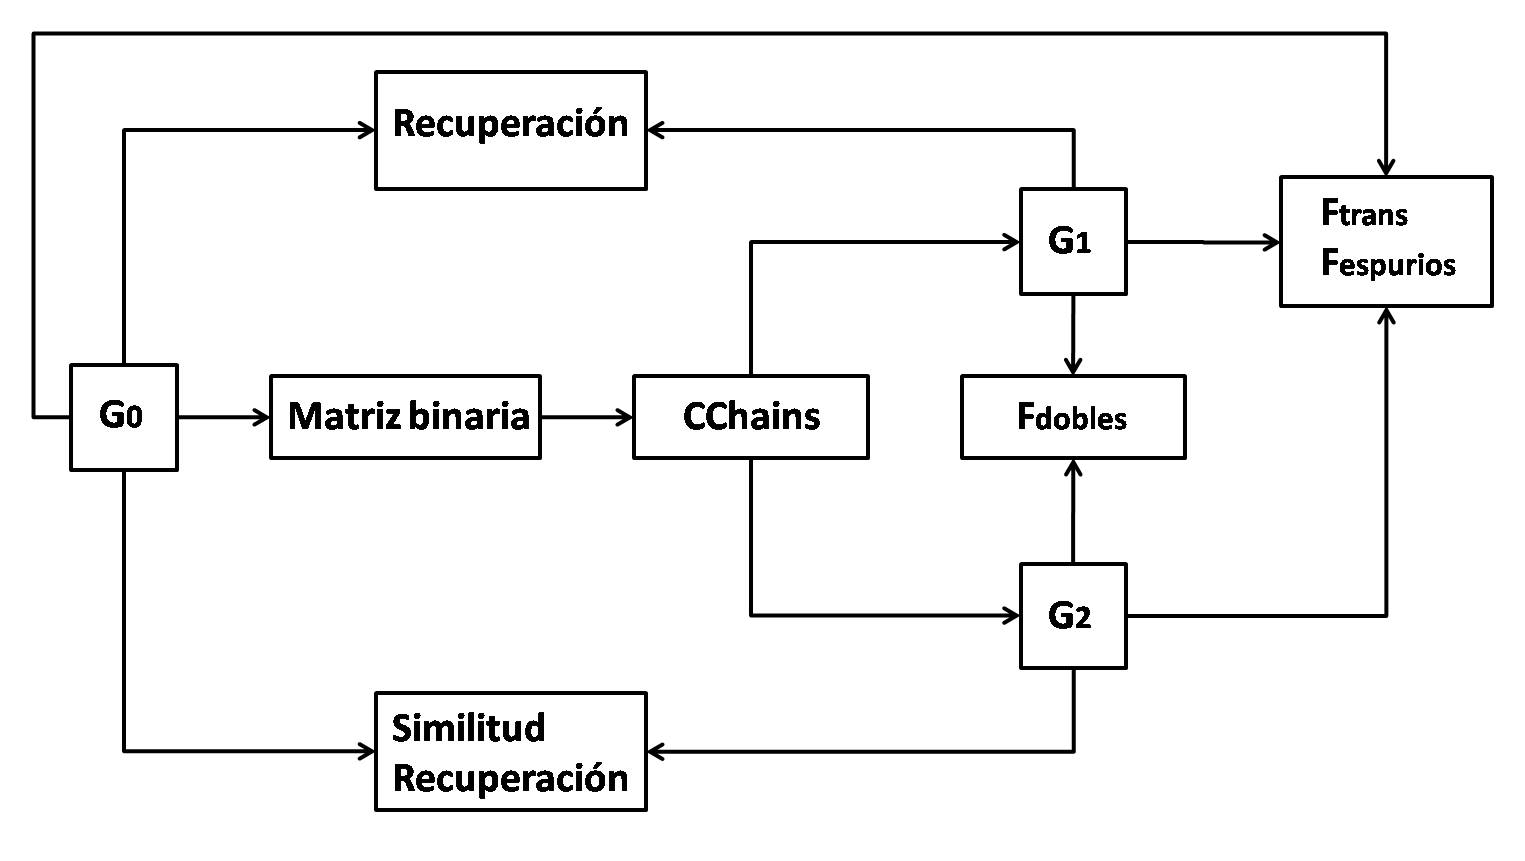
\includegraphics[width=0.85\textwidth]{diagrama.jpg}
\caption{Scheme of the algorithm validation process with synthetic data.}
\label{fig:flujo}
\end{figure}


\subsection*{Structural diversity of the test graphs}

In order to analyze the behavior of the method under different topological complexities, multiple classes of causal graphs were evaluated. Each of these types provides a different level of structural challenge for causal inference.

\begin{itemize}
    \item \textbf{Causal chains:} A chain is a linear graph in which each vertex has a single parent (except the first) and a single child (except the last), with edges of the form \( v_1 \rightarrow v_2 \rightarrow \cdots \rightarrow v_n \). This configuration represents one-dimensional causal propagation and serves as a baseline scenario for evaluating the method.

    \item \textbf{Trees:} A directed tree is a connected DAG with \( n \) vertices and \( n-1 \) edges. In this type of structure, each vertex has an in-degree less than or equal to 1, that is, at most one parent, and contains no cycles. The root is the only node without predecessors. These structures model branched causal hierarchies, characteristic of evolutionary or regulatory processes in biology. Formally, if \( T = (V, E) \) is a tree, then \( |E| = |V| - 1 \).

    \item \textbf{Forests:} A forest is a collection of disjoint trees; that is, an acyclic graph that is not necessarily connected. It can be considered the union of several independent causal subprocesses. By studying forests, variability is introduced in the number of connected components, and the response of the method to multiple unrelated partial structures is evaluated.

    \item \textbf{Graphs with immoralities:} Graphs containing immoralities are also included. These are structural patterns of the form \( A \rightarrow C \leftarrow B \), where \( A \) and \( B \) are not connected. This type of configuration introduces greater difficulty in causal inference, since the value of a vertex may depend on more than one endogenous variable. The number of immoralities was varied systematically to analyze the robustness of the method against these complex patterns.

\end{itemize}

The analysis was extended across different configurations in the number of vertices for chains and trees, the number of trees for forests, and the number of immoralities for DAGs, making it possible to establish a broader characterization of the behavior of the method in different artificial scenarios. This methodological proposal constitutes a solid basis for validating causal discovery techniques before their application to real data.




\newpage


% ====================
% Chapter 3: Results
% ====================
\chapter{Results}
\section{Computational details}

This section describes several computational details of the two classes of tasks addressed in this thesis: validation of the causal discovery algorithm on synthetic data, and its application and analysis on real gene expression data. In the validation phase, a C++ code was implemented that randomly constructs directed acyclic graphs (DAGs) and performs random sampling of the endogenous variables of the network associated with its vertices. To construct a DAG, the children of each vertex are assigned randomly using a topological order. The binary data for each vertex are obtained from the structure of the generated graph, Equations~\ref{eq:logic}, and random sampling of the exogenous variables $X_{mi}$ and $Y_{mi}$. Regarding applications to real data, gene expression profiles corresponding to clinical samples of normal and tumor tissue from patients with prostate adenocarcinoma (PRAD), lung adenocarcinoma (LUAD), or lung squamous cell carcinoma (LUSC) were downloaded\cite{prad,luad,lusc}. From these data, a preprocessing step developed in Wolfram Mathematica was used to discretize the values of the continuous gene-expression variable for each gene and each sample into binary values. These binary expression values represent states of normal or anomalous regulation of a gene in each tissue. The details of this preprocessing stage and the characteristics of the statistical sample for each tissue are addressed in Sec.~\ref{sec:prepro}. Once the binary data matrix is available, whether synthetic or real, the discovery algorithm implemented in the \texttt{CChains} software is run in order to infer the underlying causal structures. In the validation process, other ad hoc auxiliary tools were developed for the calculation of comparative metrics between graphs, as well as figures of merit for evaluating causal-discovery performance. For the processing, analysis, and visualization of the causal graphs inferred from real data, the Python computational libraries \texttt{NetworkX} and \texttt{SciPy}\cite{networkx} were used. For each of the three tissues analyzed (PRAD, LUAD, and LUSC), the adjacency lists generated by \texttt{CChains} were processed, and different centrality metrics were calculated: degree, betweenness, closeness, and \textit{PageRank}. The \texttt{NetworkX} library functions used were \texttt{degree\_centrality}, \texttt{betweenness\_centrality}, \texttt{closeness\_centrality}, and \texttt{pagerank}. 


The greatest computational cost of these tasks lies in constructing gene deregulation networks through the causal discovery algorithm. For networks with more than $n \times 10^4$ vertices, the execution time of \texttt{CChains} varies between A and B days of standard local runtime on x86\_64 architecture. Although the discovery phase is, in principle, parallelizable, the most demanding phase, responsible for graph simplification, is not. This is due to the establishment of priorities when visiting arcs for their possible removal through the Reichenbach and Mokken tests.


\section{Evaluation of the algorithm with synthetic data}


\subsection{Probability distributions for the exogenous variables}
\label{sec:generacion}

For the validation of the causal discovery algorithm implemented in \texttt{CChains}, the construction of synthetic data sets is taken as the starting point. This process involves two stages: the generation of a random reference causal graph \( G_0 \), and the subsequent creation of a binary data matrix consistent with its causal structure and with Equations~\ref{eq:logic}. From this matrix, \texttt{CChains} infers a network \( G_1 \) and a final simplified network \( G_2 \), which are compared with \( G_0 \) to evaluate the performance of the method.

\subsubsection*{Discovery region}

For a causal relationship \( i \to j \) to be inferred, it must satisfy \( \nu_i \leq \nu_j \) and \(H_{ij} > H_0 \). We consider the case of direct causal relationships present in $G_0$. Therefore, the value of the variable corresponding to the child vertex is computed through the expression \( j = (X_j \land i) \lor Y_j \). In these cases, where vertices have a single parent, the variable $X$ is represented with a single subscript indicating the vertex to which it belongs.

To guarantee that the frequencies of i and j satisfy \( \nu_i \leq \nu_j \), we assume a frequentist framework in which $\nu_i$ and $\nu_j$ identify the probabilities of variables $i$ and $j$. Taking into account the logical form of variable $j$, the probability of $j$ is then obtained as a function of $\nu_i$, $P(X_i)$, and $P(Y_i)$. Requiring $\nu_i \leq \nu_j$, we obtain:
\begin{align*}
\nu_i &\leq P((X_j \land i) \lor Y_j) \\
\nu_i &\leq \nu_i P(X_j) + P(Y_j) - \nu_i P(X_j)P(Y_j)
\end{align*}
\\
Rewriting the previous result conveniently, we have:

\begin{equation}
\label{eq:pymin}
P(Y_j) \geq \frac{\nu_i (1 - P(X_j))}{1 - \nu_i P(X_j)} \\
\end{equation}


For the calculation of the Loevinger coefficient, an analogous strategy is followed. In this case, the conditional probability of j given i is required, which yields:

\begin{equation}
\nu_{j|i} = P((X_j \land 1) \lor Y_j) = P(X_j \lor Y_j) 
\end{equation}
\\
The expression for the Loevinger coefficient becomes:
\begin{align*}
H_{ij} &= \frac{\nu_{j|i} - \nu_j}{1 - \nu_j} \\
H_{ij} &= \frac{P(X_j) + P(Y_j) - P(X_j)P(Y_j) - P(X_j) \nu_i - P(Y_j) + P(X_j) P(Y_j) \nu_i}{1 - P(X_j) \nu_i - P(Y_j) + P(X_j) P(Y_j) \nu_i}
\end{align*}
\\
Grouping and factoring terms:
\begin{align*}
H_{ij} &= \frac{P(X_j)(1 - P(Y_j)) - P(X_j) \nu_i (1 - P(Y_j))}{(1 - P(Y_j)) - P(X_j) \nu_i (1 - P(Y_j))} \\ 
H_{ij} &= \frac{P(X_j)(1 - \nu_i)}{1 - P(X_j) \nu_i}
\end{align*}
\\
Imposing the condition \( H_{ij} > H_0 = 0.5 \), we obtain:
\begin{equation}
\label{eq:zonedesc}
P(X_j) > \frac{1}{2 - \nu_{i}}, \quad P(Y_j) \neq 1
\end{equation}
\\

Equations~\ref{eq:pymin} and~\ref{eq:zonedesc} define the \textbf{discovery region}, that is, the parameter region \( (P(X_j), P(Y_j)) \) over which true relationships are guaranteed to be inferable by the algorithm. This region depends on the frequency of the parent vertex: as the parent frequency increases, the region narrows. The widest discovery region for the parameter $P(X_j)$ occurs for causal relationships in which the cause is an orphan vertex, since in that case the frequency of i is minimal.


The conditions obtained suggest the following algorithmic strategy for selecting the probabilities of the exogenous variables: 1) $P(X_j)$ is sampled in the region (\ref{eq:zonedesc}), which is completely determined by the parent vertex, and then 2) $P(Y_j)$ is sampled according to condition (\ref{eq:pymin}) and the value of $P(X_j)$ obtained in step 1.

\subsubsection*{Validation of the Reichenbach test: elimination of spurious arcs}

We now consider the case of a graph with structure \( i \leftarrow k \rightarrow j \), where \( i \) and \( j \) share a common parent \( k \). Given the binary data, \texttt{CChains} could construct a spurious arc \( i \to j \), which should be eliminated by the Reichenbach test. The corresponding logical expressions are:

\begin{align*}
i &= (X_i \land k) \lor Y_i \\
j &= (X_j \land k) \lor Y_j
\end{align*}
\\
To find the conditions on P(X) and P(Y) that allow the elimination of a possible spurious arc $ i \to j $, we develop the inequalities of the Reichenbach test in this case. First, the conditional frequencies are calculated:
\begin{align*}
\nu_{ij|k} &= P((X_i \lor Y_i)P(X_j \lor Y_j)) \\
\nu_{ij|\neg k} &= P(Y_i \land Y_j) = P(Y_i) P(Y_j)) \\
\nu_{i|k} &= P(X_i \lor Y_i)  \\ 
\nu_{j|k} &= P(X_j \lor Y_j)  \\
\nu_{i|\neg k} &= P(Y_i) \\
\nu_{j|\neg k} &= P(Y_j)
\end{align*}
\\
These expressions lead to:
\begin{align}
\nu_{ij|k} - \nu_{i|k} \nu_{j|k} &= 0 \\
\nu_{ij|\neg k} - \nu_{i|\neg k} \nu_{j|\neg k} &= 0
\end{align}
\\
In this way, it is guaranteed that \( H_{ij|k} = H_{ij|\neg k} \leq 0.5 \) for all $P(X_i)$, $P(Y_i)$, $P(X_j)$, and $P(Y_j)$. This means that the Reichenbach test correctly eliminates spurious arcs, independently of the distribution of the exogenous variables.

\subsubsection*{Compatibility of Reichenbach with real arcs}

This section analyzes whether the Reichenbach test could incorrectly eliminate a real arc in the causal chain \( k \to i \to j \). If the graph includes a transitive arc \( k \to j \), then \( k \) is considered a common parent of \( i \) and \( j \), and the validity of \( i \to j \) could be evaluated; see Figure~\ref{fig:reich}.

We start from the logical expressions:
\begin{align}
i &= (X_i \land k) \lor Y_i \\
\label{eq:ij}
j &= (X_j \land i) \lor Y_j = (X_j \land ((X_i \land k) \lor Y_i)) \lor Y_j
\end{align}
\\
From these, the relevant frequencies are calculated:

\begin{align*}
\nu_{ij} &= P((X_i \land k) \lor Y_i) (P(X_j) + P(Y_j) - P(X_j)P(Y_j))\\
\nu_{ij|k} &= P(X_i \lor Y_i) P(X_j \lor Y_j) \\
\nu_{ij|\neg k} &= P(Y_i) P(X_j \lor Y_j) \\
\nu_{i|k} &= P(X_i \lor Y_i) \\
\nu_{i|\neg k} &= P(Y_i) \\
\nu_{j|k} &= P(X_j)P(X_i \lor Y_i) + P(Y_j) - P(Y_j)P(X_j)P(X_i \lor Y_i) \\
\nu_{j|\neg k} &= P(X_j)P(Y_i) + P(Y_j) - P(X_j) P(Y_i) P(Y_j)
\end{align*}
\\
Substituting into the conditioned Loevinger coefficients (\ref{eq:reichenbach}), the conditions under which the Reichenbach test would eliminate the real arc $i \to j$ are obtained:
\begin{align}
2 P(X_j \lor Y_j) -\nu_{j|k} &\leq 1 \\
2 P(X_j \lor Y_j) -\nu_{j| \neg k} &\leq 1
\end{align}
\\
These must be jointly satisfied for the elimination of the arc; therefore, it is enough to guarantee that at least one of them is not satisfied in order to preserve $i \to j$. Developing the second inequality, using the expression for $\nu_{j| \neg k}$, we obtain:
\begin{equation}
\label{eq:region}
P(X_j)(2 - P(Y_i)) \leq 1, \quad P(Y_j) \neq 1
\end{equation}
\\
To avoid trivial frequencies in $j$, $P(Y_j) \neq 1$. Thus, the region in which the Reichenbach test does not eliminate the real arc is written as: 
\begin{equation}
\label{eq:muestreo}
P(X_j) > \frac{1}{2 - P(Y_i)}
\end{equation}
\\
Since for every vertex i it holds that $P(Y_i) \leq \nu_i$, the previous region is contained within the discovery region, Equation~\ref{eq:muestreo}. Therefore, for all values of \( P(X) \) and \( P(Y) \) within the discovery region, Reichenbach will not eliminate real arcs in the average case.

\begin{figure}[h!]
\centering
\begin{subfigure}[b]{0.2\textwidth}
	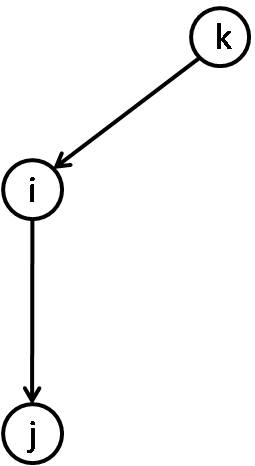
\includegraphics[width=\textwidth]{reich1.jpg}
	\caption{}
	\label{fig:reich1}
	\end{subfigure}
	\hfill
\begin{subfigure}[b]{0.2\textwidth}
	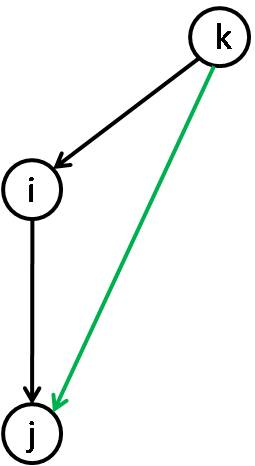
\includegraphics[width=\textwidth]{reich2.jpg}
	\caption{}
	\label{fig:reich2}
	\end{subfigure}
	\hfill
\begin{subfigure}[b]{0.2\textwidth}
	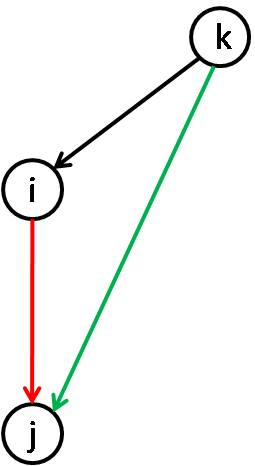
\includegraphics[width=\textwidth]{reich3.jpg}
	\caption{}
	\label{fig:reich3}
	
\end{subfigure}
\hfill

\caption{Representation of a 3-vertex chain, its transitive edge, and the edge to be analyzed by the Reichenbach test, represented in green and red.}
\label{fig:reich}
\end{figure}

\subsubsection*{Evaluation of the Mokken test: elimination of transitive arcs}

The Mokken test is designed to identify and eliminate transitive arcs in triangles of mutually linked vertices. In triangles, the length of side i $ \to $ j is defined as $ | \nu_i - \nu_j | $, and the hypotenuse of the triangle is defined as the side with the greatest length. Given a causal triangle \( i \to j \to k \), the transitive arc \( i \to k \) always represents its hypotenuse. 
The logical expressions of the vertices are: 

\begin{align*}
i &= Y_i \\
j &= (X_j \land i) \lor Y_j \\
k &= (X_k \land j) \lor Y_k
\end{align*}
\\
Using a particular case in which we assume that the pairs of values $P(X)$ and $P(Y)$ are equal for every vertex, we obtain the following expressions for the frequencies:

\begin{align*}
\nu_{ij} &= \nu_i (P(X) + P(Y) - P(X)P(Y)) \\
\nu_{jk} &= \nu_j (P(X) + P(Y) - P(X)P(Y)) \\
\nu_{ik} &= \nu_i P(Y) + (1 - P(Y))P(X) \nu_{ij} \\
\nu_{\neg i \neg j} &= \nu_{\neg i}(1 - P(X) P(Y)) \\
\nu_{\neg j \neg k} &= \nu_{\neg j}(1 - P(X) P(Y)) \\
\nu_{\neg i \neg k} &= \nu_{\neg i}(1 - P(Y))(1 - P(X)) + P(X)(1 - P(Y)) \nu_{\neg i \neg j} 
\end{align*}
\\
where $\nu_{\neg i} = 1 - \nu_i$ and $\nu_{\neg i \neg j}$ is the frequency of zero coincidences in variables $i$ and $j$.
\\

These expressions satisfy the Mokken conditions when the following relations hold:
\begin{equation}
\label{eq:mokken}
\nu_i = \nu_{ij} \quad,  \nu_i =\nu_{ik} \quad, \quad \nu_{j} = \nu_{jk}
\end{equation}
\\
These are equivalent to $[0 \mathrm{errors}]_{ijk} =$ total number of samples. This situation is obtained when $P(X) = 1$.
\\

In the more general case, it is difficult to find conditions for $P(X_i)$ and $P(X_j)$ that jointly allow the elimination of transitive arcs. In what follows, we will assume only the restrictions on $P(X_i)$ and $P(X_j)$ given above, which guarantee the discovery and preservation of direct causal relationships, even when they do not allow a transitive edge to be eliminated using the Mokken criterion.




It should be noted that transitive arcs also represent causal relationships, and they are eliminated mainly to reduce graph complexity and facilitate analysis. Therefore, the operation of the Mokken test is not as critical as that of Reichenbach, which can compromise the validity of the inference if it does not correctly detect spurious arcs. This analysis guarantees that the parameter region selected for \( P(X) \) and \( P(Y) \) in the generation of synthetic data makes it possible to discover true relationships, eliminate spurious arcs, and simplify transitive arcs under certain conditions of exogenous noise without compromising the causal integrity of the graph.





\subsection{Reconstruction of causal graphs}

In validating the algorithm, different types of graphs were considered in order to cover a representative structural diversity: causal chains, trees, forests, and graphs with immoralities (v-structures). These configurations make it possible to evaluate the behavior of the method both in simple scenarios and in topologically more complex structures.

For each class of graph and for each fixed number of vertices, 500 different graphs were generated randomly in order to guarantee the statistical convergence of the metrics obtained. The number of samples per vertex, that is, the number of columns in the binary data matrix, was set equal to 500. This quantity was considered sufficient to stabilize the absolute and conditional frequencies used in the inferential process.

The causal model is not completely defined by generating a random graph $G_0$ under the topological restrictions mentioned above (chains, trees, forests, and DAGs with immoralities). For its complete definition, it is also necessary to specify the probabilities of the exogenous variables associated with each vertex. In Section~\ref{sec:2.3}, conditions were derived for these probabilities that would allow, in the average case, the recovery of causal relationships through the criterion of the proposed method. In the generation of synthetic data, we begin by randomly sampling the values of $P(X_i)$ and $P(Y_i)$, following uniform distributions restricted to the intervals compatible with those theoretical conditions. In practice, additional restrictions are imposed. $P(Y_i)$ has no nontrivial upper bound according to our first analyses. Nevertheless, in the cases studied, $P(Y)$ is set $< 1/2$. This requirement prevents the frequency of some vertices from rapidly reaching its maximum value, which would compromise the variability required to establish causal relationships.

If there are no further restrictions on the values of $P(X)$, they can approach the lower threshold $P_{min} \neq 0$. In that case, sampling the values of variable X with probability $P(X)$ can lead to effective frequencies of X lower than $P_{min} = \frac{1}{2 - \nu_i} \neq 0$. As a consequence, causal discovery, in terms of absolute and conditional frequencies, would not work. To guarantee more robust causal discovery, an additional restriction is imposed. In a frequentist interpretation of probabilities, $P(X)$ is the limiting frequency when sampling is extended infinitely. If finite data are available, the effective frequencies follow a binomial distribution, with mean $P(X)$ and standard deviation $\sqrt{P(X)(1 - P(X))}$. Thus, the vast majority of effective frequencies will lie in the interval from $P(X) - \sqrt{P(X)(1 - P(X))}$ to $P(X) + \sqrt{P(X)(1 - P(X))}$. Therefore, a possible strategy to mitigate the problem mentioned in the previous paragraph, namely that some effective frequencies of X do not allow causal discovery, is to impose the following inequality:

\begin{equation}
\label{eq:omega}
P(X) -\sqrt{P(X)(1 - P(X))} > \frac{1}{2 - \nu_i}
\end{equation} 
\\ 
This approach is equivalent to taking a safety margin of one standard deviation below the expected value $P(X)$, and it can be interpreted as a discovery threshold under uncertainty. In this way, the statistics involved in data generation are prevented from introducing omission errors for real causal relationships.  

At first glance, this procedure could suggest a bias in the validation, since it uses information derived from the causal discovery method itself. However, this design does not guarantee discovery success in particular instances. Once the values of $P(X_i)$ and $P(Y_i)$ have been obtained, the values of the endogenous variables are sampled using the structure of graph $G_0$, the structural equations, and random realizations of the exogenous variables according to their probabilities. Therefore, in each execution, the sampled probabilities are translated into empirical frequencies that differ from the theoretical values, introducing variability that may be significant. The purpose of this protocol is therefore to validate the method under nontrivial conditions, where success is not organized but is reasonably expected according to the theory. It should be noted that the conditions for the probabilities of the exogenous variables were obtained under restricted structural assumptions, such as chains, trees, or forests, where each vertex has a single parent. In more general directed acyclic graphs, which may include immoralities and multiple parents per node, the parameter space remains largely unexplored, leaving open ground for the empirical validation of the method.


The algorithm for generating the synthetic data matrix starts from the orphan vertices, whose logical expression depends only on variable $Y$. In these cases, the value of $P(Y)$ used is randomly chosen between 0.1 and 0.15. For each sample in the data-matrix row of these vertices, a random value q uniformly distributed in the interval [0,1] is generated; if q $< P(Y)$, the sample takes value 1, otherwise it takes value 0.
After generating the data corresponding to the orphan vertices, sampling proceeds for the remaining vertices of the graph. For each child vertex j with parent(s) i, the following steps are followed:

\begin{itemize}
\item The frequency $\nu_i$ of parent i is calculated in the corresponding row of the data matrix. From this frequency, a minimum admissible value $P_{min}$ for $P(X)$ is determined according to Equation~\ref{eq:omega}.
\item A random value $P(X)$ uniformly distributed in the interval [$P_{min}$,1] is generated. Using this value, the corresponding minimum $P_{min}$ for the probability $P(Y)$ is calculated through Equation~\ref{eq:pymin}, and $P(Y)$ is finally generated as a uniform random value in the interval [$P_{min}$,0.5].
\item With the values of $P(X)$ and $P(Y)$ defined, the value of vertex j in each sample n is generated according to the logical formula established in Equation~\ref{eq:logic}. In the cases of chains, trees, and forests, the element corresponding to the nth sample is expressed as:
	\begin{equation*}
		M_{jn} = (M_{in} \land X_j) \lor Y_j
	\end{equation*}
\\
For the sampling of $X_j$ and $Y_j$, a random number uniformly distributed in the interval [0,1] is generated for each variable. If the number corresponding to variable $X_j$ is smaller than $P(X)$, then $X_j = 1$; otherwise, $X_j = 0$. Analogously, if the second number is smaller than $P(Y)$, then $Y_j = 1$; otherwise, $Y_j = 0$. 

In the case of graphs with immoralities, sampling is specified differently. The value of $P(X)$ for variable $X$ is calculated as a function of the frequency of the parent i that accompanies it in the logical expression, whereas $P(Y)$ is generated using the frequency $\nu_i$ of the parent with the largest value among those influencing j. This preserves the statistical conditions necessary for causal relationships between vertices to be inferred.
\end{itemize} 
     

From the obtained data matrix, the \texttt{CChains} code constructs a graph $G_1$ and subsequently its simplified version $G_2$. These graphs, together with $G_0$, are used to quantitatively evaluate the accuracy of the algorithm through the calculation of the metrics defined in Section~\ref{sec:2.3}.



\subsection{Performance metrics}
\subsubsection{Causal chains}
Causal chains constitute the simplest structural configuration for a causal network, with linear propagation of information from one vertex to the next. Due to the graph structure in this case, the main problem is transitive edges and the possible undirected edges constructed in graph $G_1$, since there will be no spurious edges. First, the case of 15-vertex chains with $P(X_i) = P(X)$ for every vertex is treated. Figure~\ref{fig:chain_x} shows the behavior of the performance metrics as a function of $P(X)$ in this case. The fractions increase to values very close to 1 for P(X)=1, an expected result given the conditions established in Equation~\ref{eq:mokken}.

Given the structural equations in this case ($j=(i \land X) \lor Y_j$, if $j$ is not orphan), the mean error frequency for the causal relationship $i \to j$ is $1 - P(X) - P(Y_j) + P(X)P(Y_j)$. Since $P(Y_j) > 0$, $1 - P(X) - P(Y_j) + P(X)(Y_j) > 1 - P(X) - P(Y_j)$. Therefore, the lower $P(X)$ is, the larger the number of errors in $i \to j$. This is why low values of $P(X)$ compromise the discovery fraction in the inferred graphs. This behavior is seen in Figure~\ref{fig:chain_x}, where the discovery fraction grows monotonically as a function of $P(X)$, from 20$\%$ of the real edges discovered for $P(X)=0.6$ to 100$\%$ exactly for $P(X)=1$. 

On the other hand, Figure~\ref{fig:chain_x} shows that the fraction of eliminated transitive edges $F_{trans}$ is high for low values of $P(X)$. As $P(X)$ decreases, errors increase for causal relationships between any pair of vertices in the chain, and therefore the corresponding Loevinger coefficient becomes progressively smaller. This leads to a reduction in the discovery of transitive edges in the low-$P(X)$ regime, to the point that no transitive edge is discovered in the reconstructed graph for $P(X)=0.6$, that is, $|E_t(G_1)=0|$. Since $G_2$ is a simplification of $G_1$, $|E_t(G_1)=0|$ implies $|E_t(G_2)=0|$. According to the definition of the fraction of eliminated transitive edges, $F_{\text{trans}} = 1 - \frac{|E_{\text{t}}(G_2)|}{|E_{\text{t}}(G_1)|}$ is undefined in this case. To avoid unnecessarily penalizing a context in which the algorithm is not operating incorrectly, the exceptional value $F_{\text{trans}} = 1$ is chosen. 

As $P(X)$ increases, the number of errors decreases and a larger number of edges is discovered (including transitive ones). However, the elimination of transitive edges is also affected by the number of errors. In fact, as we saw in Section~\ref{sec:cchains}, the Mokken conditions can be written as an ordering from lower to higher frequencies of patterns with two errors, one error, and zero errors in three vertices connected by a directed path. This error criterion in the data is more restrictive than the discovery criterion, involving three vertices instead of two. Thus, it will be necessary to further decrease the number of errors in order to eliminate a previously discovered transitive edge; see an example in Figure~\ref{fig:transitive}. This is the origin of the decrease in $F_{trans}$ as $P(X)$ increases, down to its minimum at $P(X)= 0.99$.  

The behavior of the similarity between the original and reconstructed graph reflects the behavior of the different fractions used. A global measure of this type may lead one to think that causal discovery is not effective. However, a low capacity to reconstruct the original graph does not necessarily invalidate the \texttt{CChains} algorithm. In particular, if the original graph only indicates direct connections between vertices (as in our case), the similarity between the original and inferred graph may be small solely because of the presence of transitive arcs in the inferred graph. Note, however, that transitive edges also represent causal relationships, although indirect ones. It is desirable to eliminate transitive edges from a graph in order to simplify its interpretation and reduce redundant information, but doing so is not strictly necessary. A causal discovery process remains valid even if it generates causal graphs containing transitive edges.

The fraction of eliminated double arcs for intermediate values of $P(X)$ is not maximal. This means that the conditions imposed in the generation of $P(Y_j)$ only guarantee that $\nu_i \leq \nu_j$ holds on average for every pair (i,j) with i parent of j.

For large values of $P(X)$, small differences are observed between the discovery fractions in $G_1$ and $G_2$. These differences are due to specific cases in which real arcs are eliminated during the simplification phase of the algorithm. This occurs because vertices with many ancestors assume large frequencies, becoming indistinguishable for pairs of parent-of-parent and child ($i$,$j$) that are far from the orphan vertex. This causes the directed edge $j \to k$ to be eliminated by the Reichenbach test due to the existence of a transitive edge $i \to j$, which establishes i as a common parent of $j$ and $k$. This is because, since i, parent of j, and j are identical, the relations $\nu_{jk|i} = \nu_{k|i}$, $\nu_{j|i} = 1$, $\nu_{jk| \neg i} = 0$, and $\nu_{j| \neg i} = 0$ are obtained. These conditions imply that $H_{jk|i} = 0$ and $H_{jk| \neg i} = 0$ in those cases. However, these are situations in which correct causal discovery cannot be expected, because it is not possible to infer causal relationships between $i$ and $j$, or to distinguish the causal relationships that $i$ and $j$ have with third vertices, if $i$ and $j$ are indistinguishable.


This problem is not exclusive to synthetic data. Cases of vertex indistinguishability also occur in real data. Nevertheless, before running the causal discovery algorithm on real data, a vertex-compression process is performed, which leads several variables from the original data to be associated with the same node of the causal graph. Under these conditions, the inferred causal relationships would only indicate that one of the variables of the $"$compressed$"$ node (without specifying which one) may be causally associated with another variable external to it.


To evaluate the ability of the algorithm to reconstruct more complex causal chains, their diameter was increased. This time, the values of both exogenous variables are distributed with probabilities $P(X_i)$ and $P(Y_i)$ that depend on the vertex (see expressions~\ref{eq:zonedesc} and~\ref{eq:pymin}, respectively). This guarantees that causal discovery in $G_1$ is effective on average, and makes it possible to evaluate the success of the algorithm in the graph simplification phase. The behavior of the performance metrics as the graph order increases is shown in Figure~\ref{fig:chain_n}.

It is observed that the algorithm maintains high performance in the fractions of eliminated spurious and double edges, as well as in the discovery fractions in $G_1$ and $G_2$. These fractions tend to decrease for chains with more than 10 vertices, which is due to the possible appearance of indistinguishable vertices. However, this behavior does not represent a practical limitation, since it is observed for diameters larger than those characteristic of real biological networks\cite{borner}.

\begin{figure}[H]
\centering
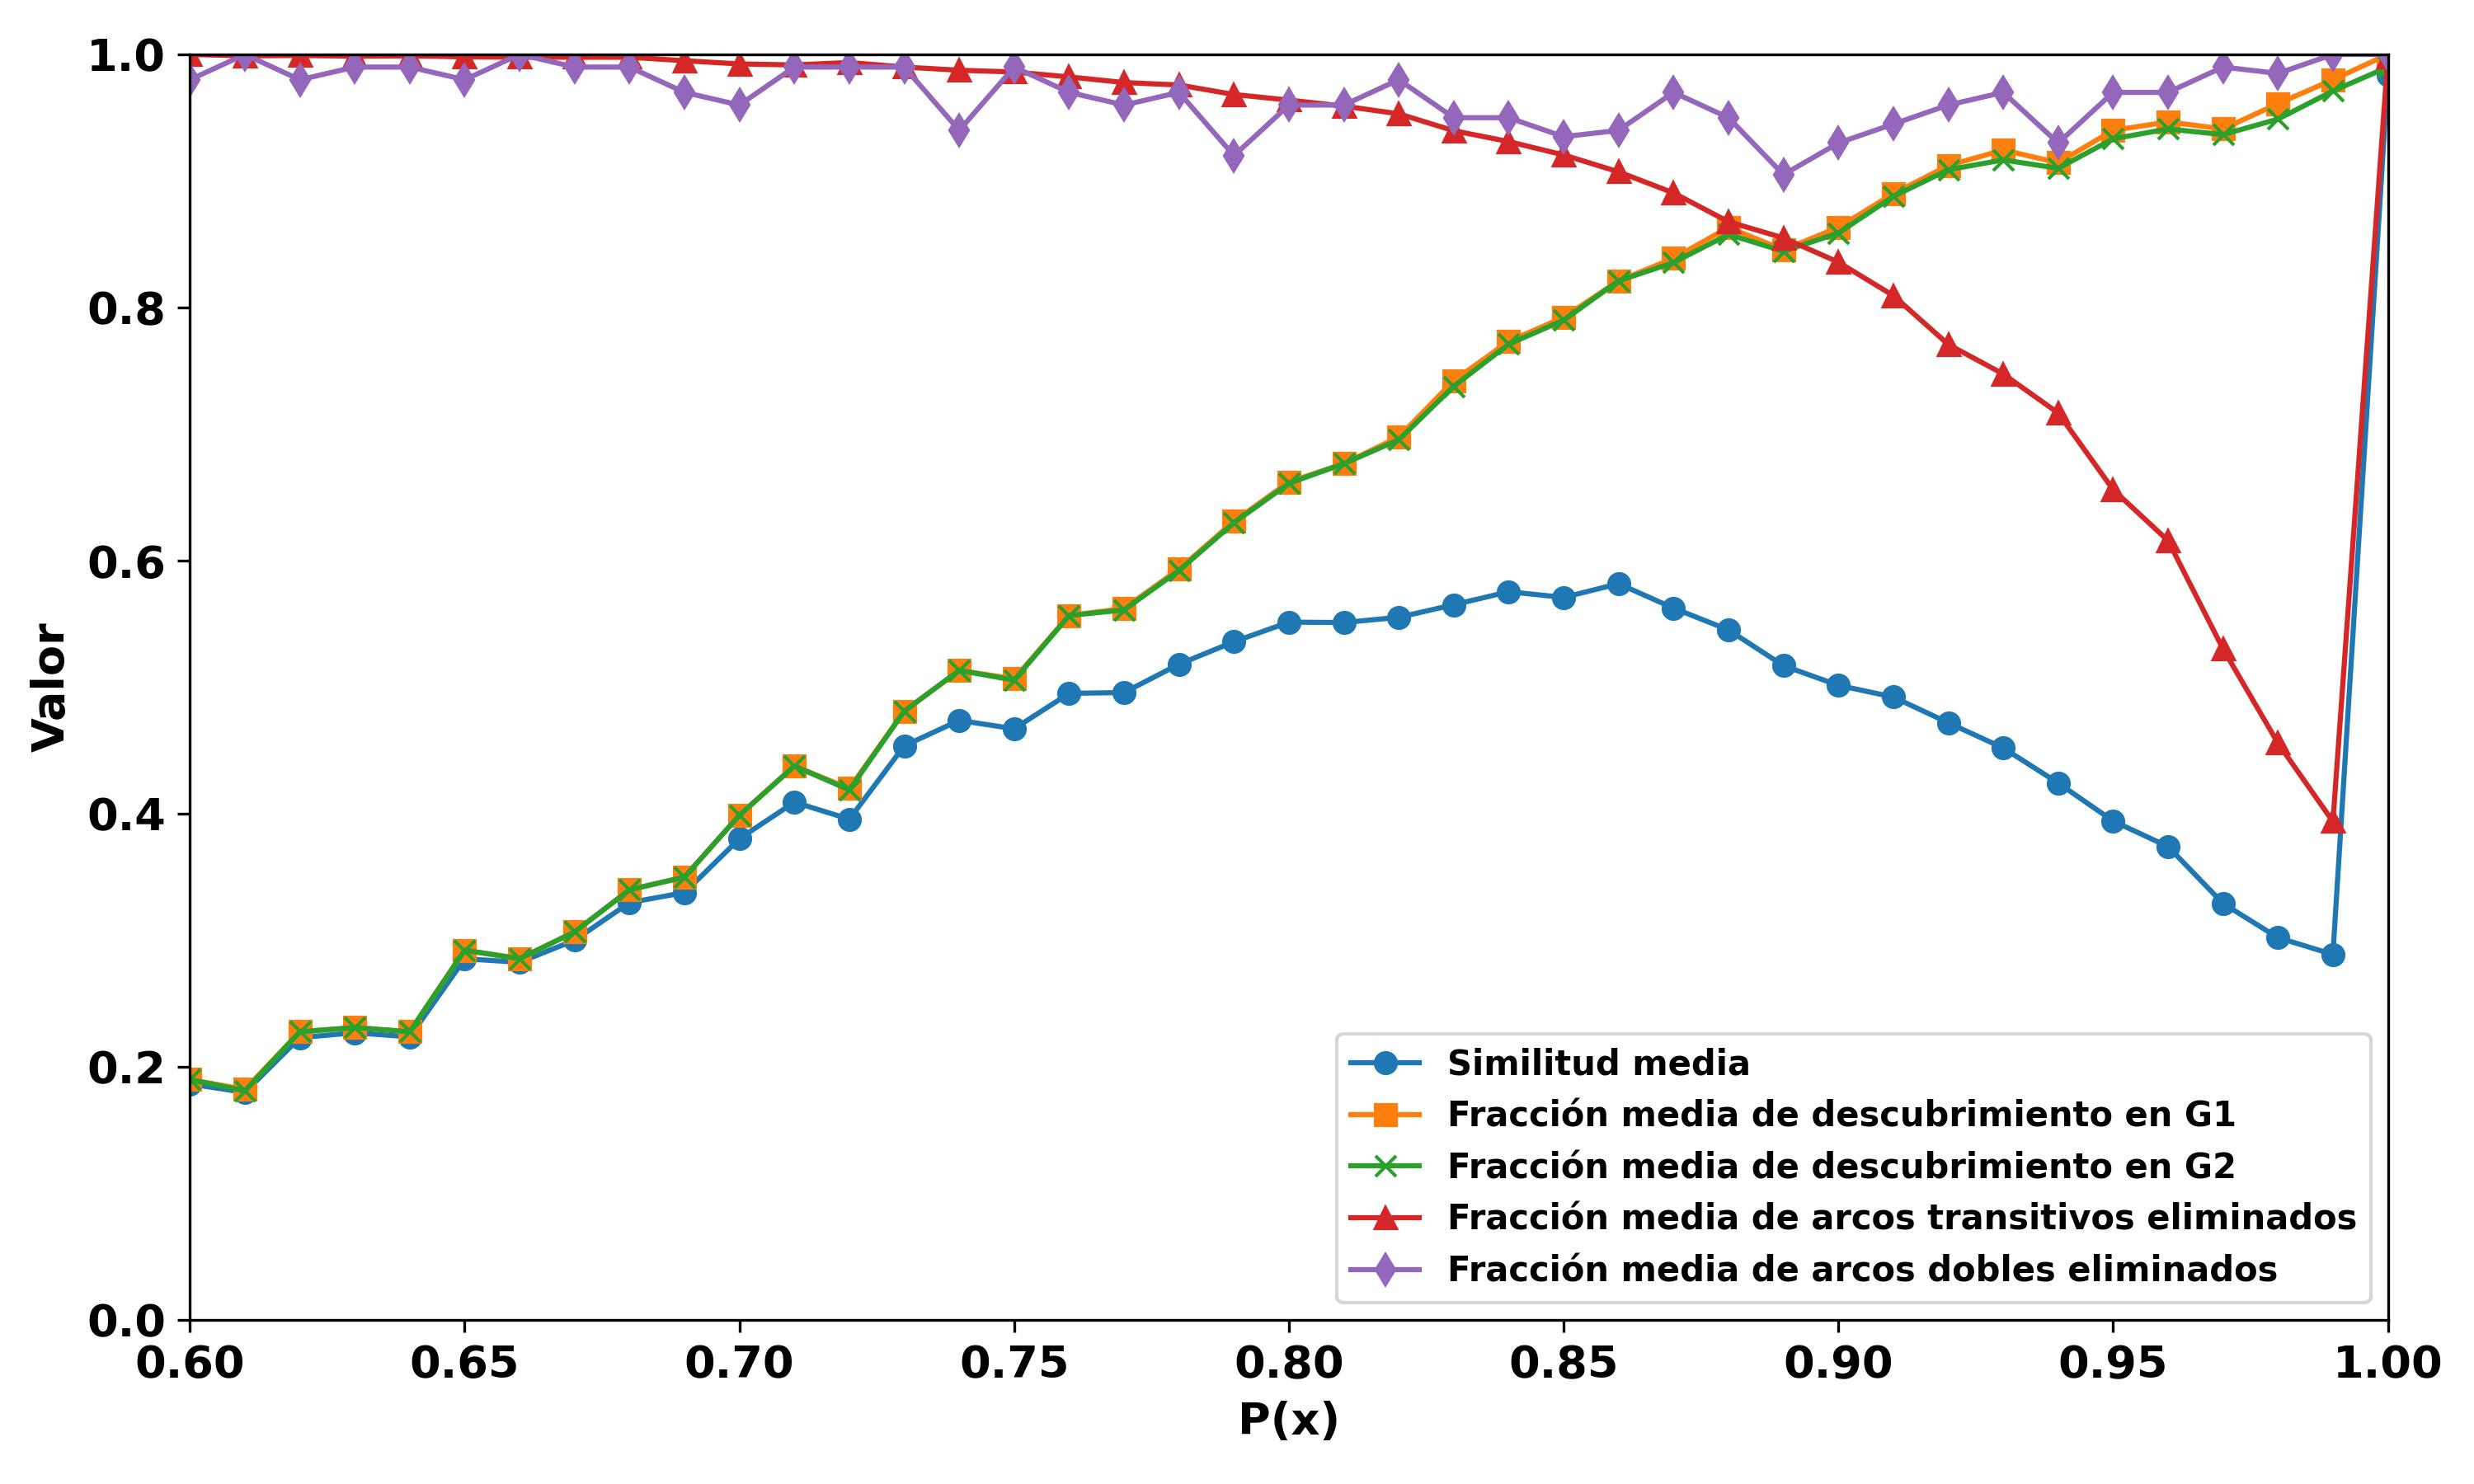
\includegraphics[width=1\textwidth]{chain_x.jpg}
\caption{Performance metrics for each P(X), in 15-vertex chains.}
\label{fig:chain_x}
\end{figure}

\begin{figure}[h!]
\centering
\begin{subfigure}[b]{0.2\textwidth}
	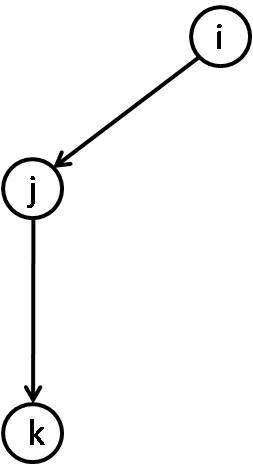
\includegraphics[width=\textwidth]{transitive1.jpg}
	\caption{$P(X)=0.6$, $F_{trans}=1$}
	\label{fig:transitive1}
	\end{subfigure}
	\hfill
\begin{subfigure}[b]{0.2\textwidth}
	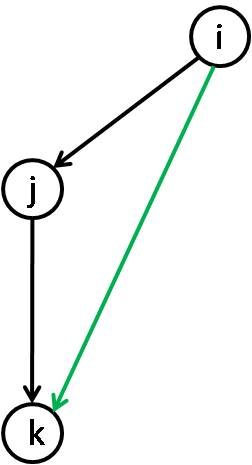
\includegraphics[width=\textwidth]{transitive2.jpg}
	\caption{$P(X)=0.9$, $F_{trans}=0$}
	\label{fig:transitive2}
	\end{subfigure}
	\hfill
\begin{subfigure}[b]{0.2\textwidth}
	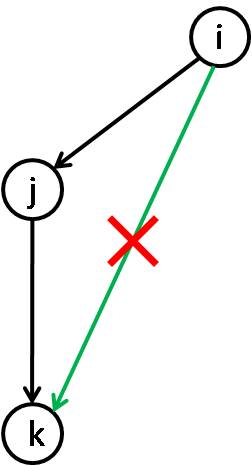
\includegraphics[width=\textwidth]{transitive3.jpg}
	\caption{$P(X)=1$, $F_{trans}=1$}
	\label{fig:transitive3}
	
\end{subfigure}
\hfill

\caption{Example of construction and simplification of the chain $i \rightarrow j \rightarrow k$ for three values of $P(X)$.}
\label{fig:transitive}
\end{figure}

\begin{figure}[H]
\centering
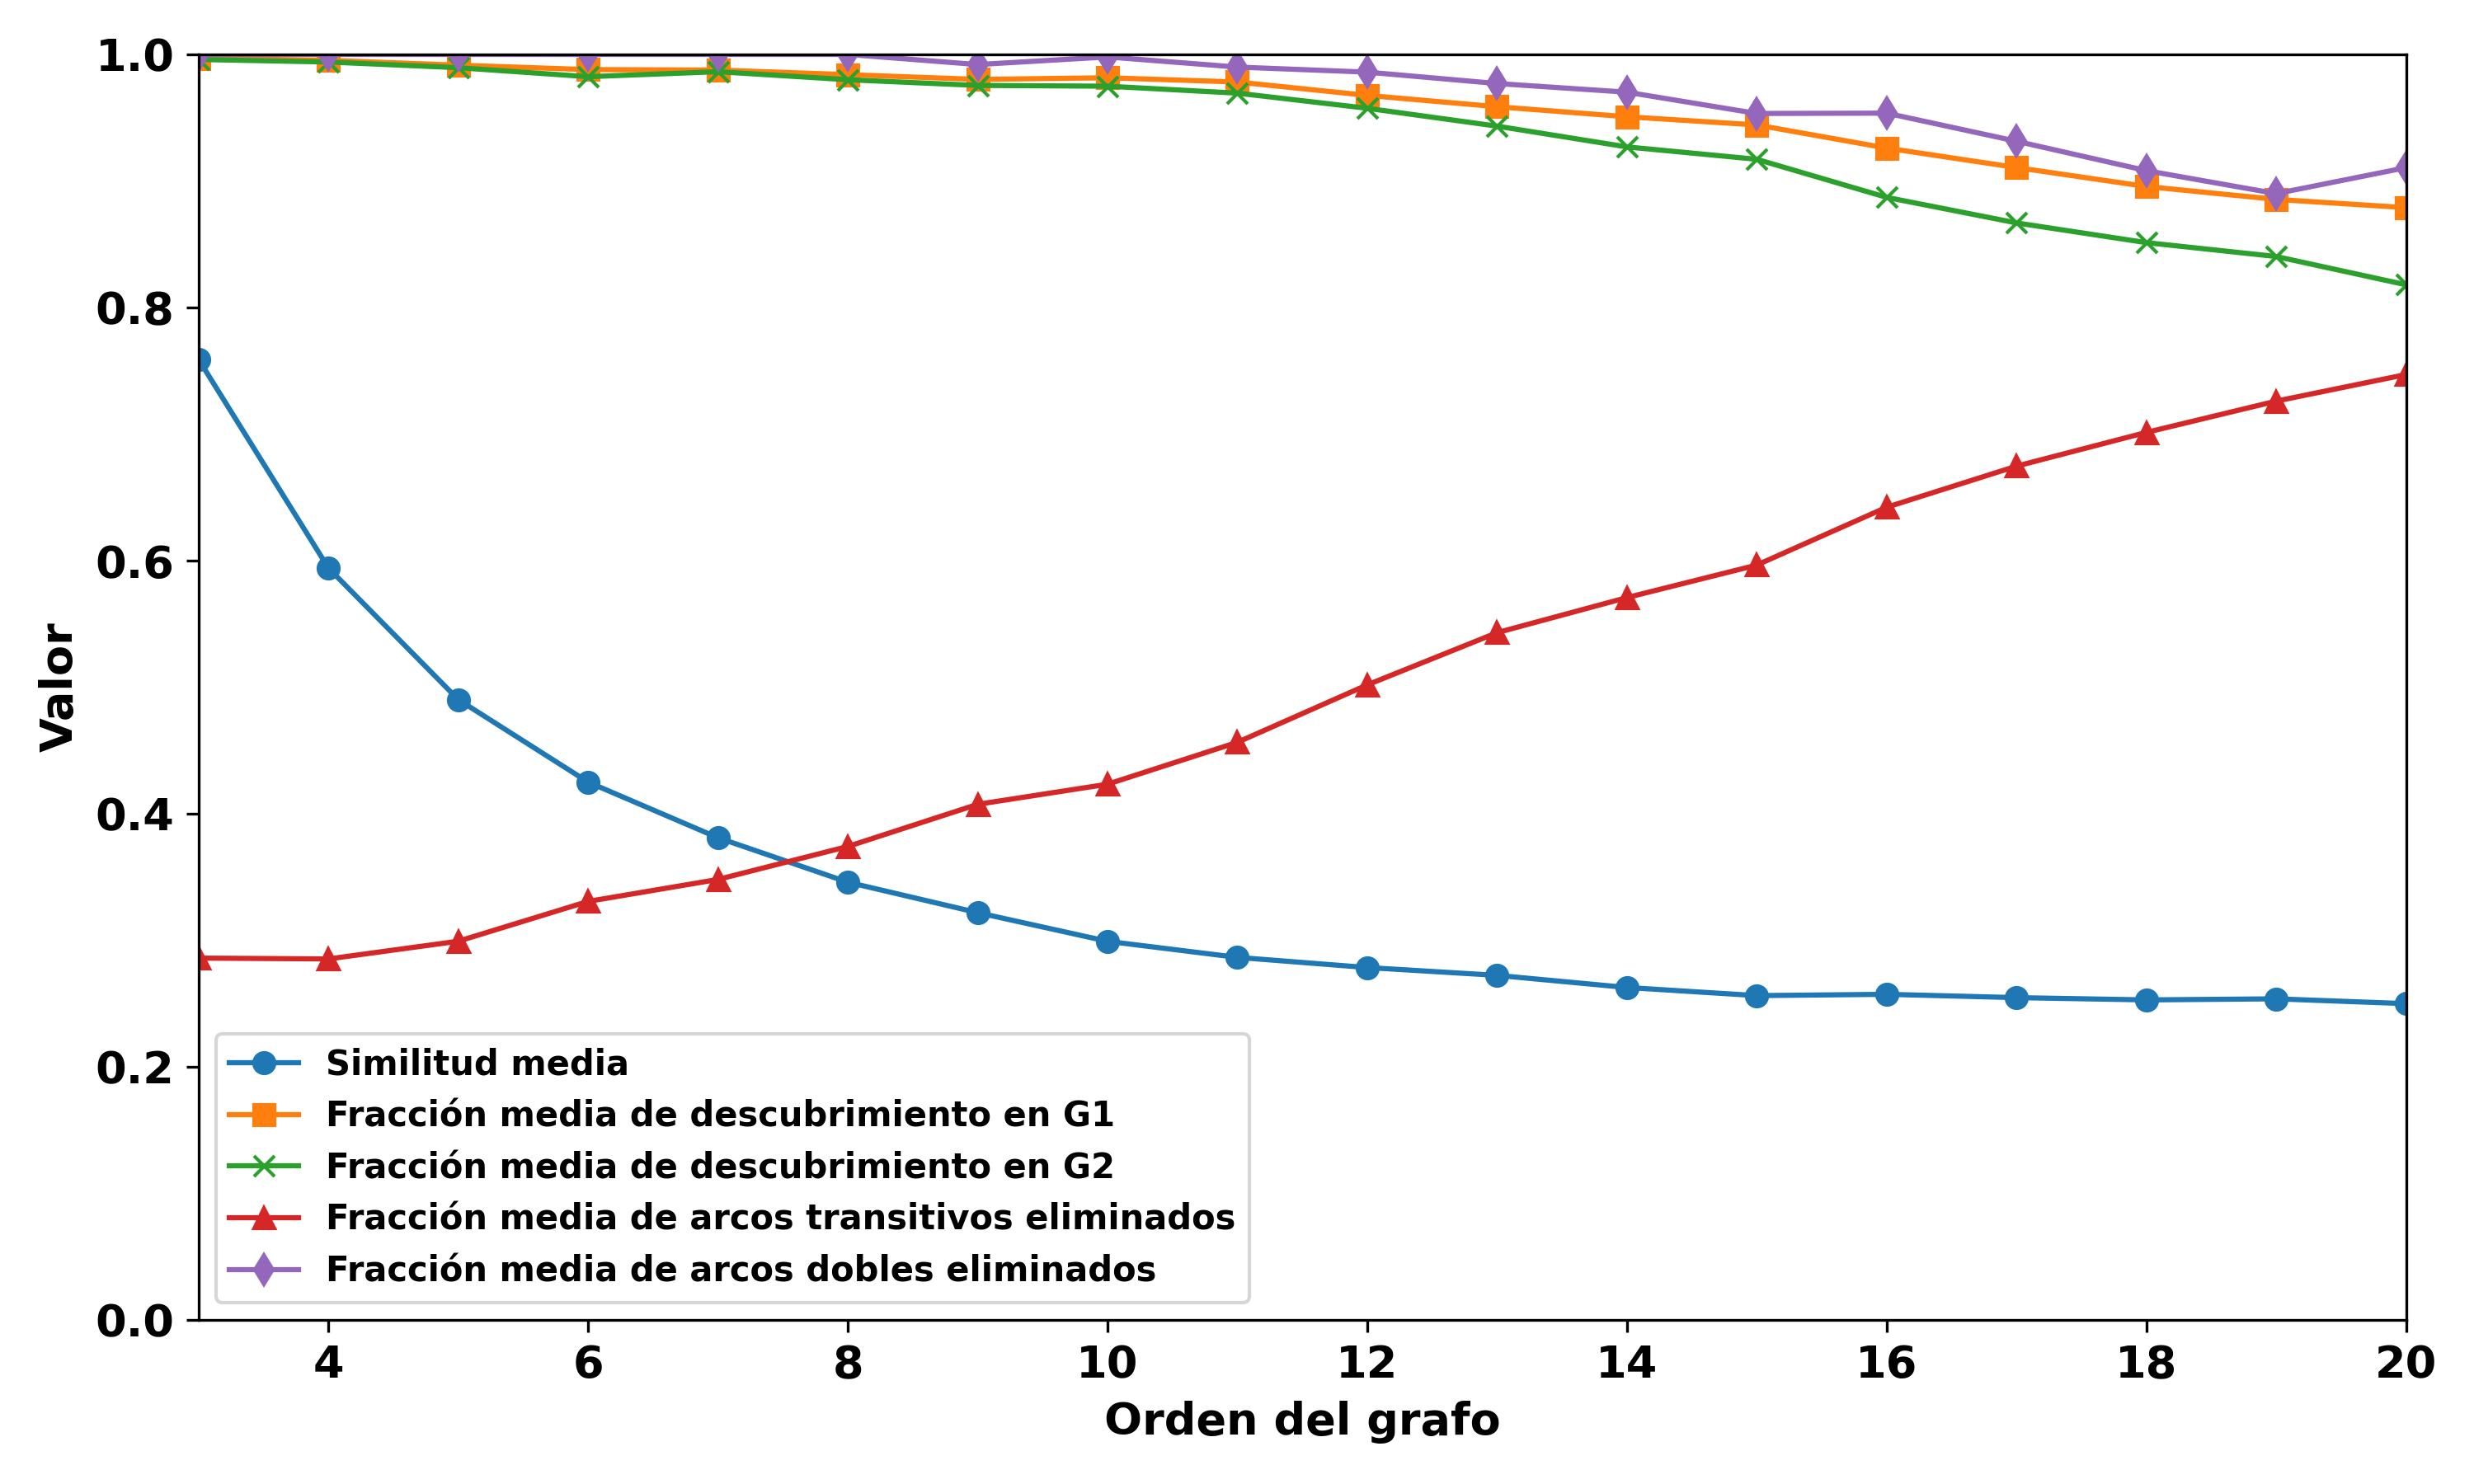
\includegraphics[width=1\textwidth]{chain_n.jpg}
\caption{Performance metrics for each graph order, in chains.}
\label{fig:chain_n}
\end{figure}

\subsubsection{Trees}

Trees add complexity by introducing a hierarchical branching structure, where multiple vertices may share a common ancestor. Unlike causal chains, in this case, when reconstructing the causal graph, spurious edges may be obtained that should be eliminated by the Reichenbach test. It is therefore necessary to verify the correct operation of the Reichenbach test for detecting and eliminating such edges. Additionally, it must be verified that the Reichenbach test is unable to eliminate edges of the reference graph corresponding to true (non-spurious) causal relationships. Similarly to the case of causal chains, we first analyze 15-vertex trees with $P(X_i) = P(X)$ for every vertex in the graph. Figure~\ref{fig:tree_x} shows how the performance metrics vary as a function of $P(X)$. A high fraction of eliminated double and spurious arcs is observed. The discovery fractions in $G_1$ and $G_2$ differ slightly from $P(X) \approx 0.88$ onward, a behavior similar to that described for chains. As in the previous case, the origin of this discrepancy lies in the indistinguishability of high-frequency connected vertices.

Figure~\ref{fig:tree_n} shows the performance metrics as a function of graph order. In this analysis, the values of the exogenous variables are distributed with probabilities $P(X_i)$ and $P(Y_i)$ according to Equations~\ref{eq:zonedesc} and~\ref{eq:pymin}, respectively. Adequate performance is observed in the recovery of the original graph, supported by the elimination of most spurious and double edges in $G_2$, as well as by a significant discovery fraction of real edges that are preserved in graph $G_2$. The low similarity values are exclusively a consequence of a low fraction of eliminated transitive edges. Note that the problems affecting the performance of the \texttt{CChains} algorithm for long chains also appear for trees with many vertices, since the branches of a tree also constitute chains.  

\begin{figure}[H]
\centering
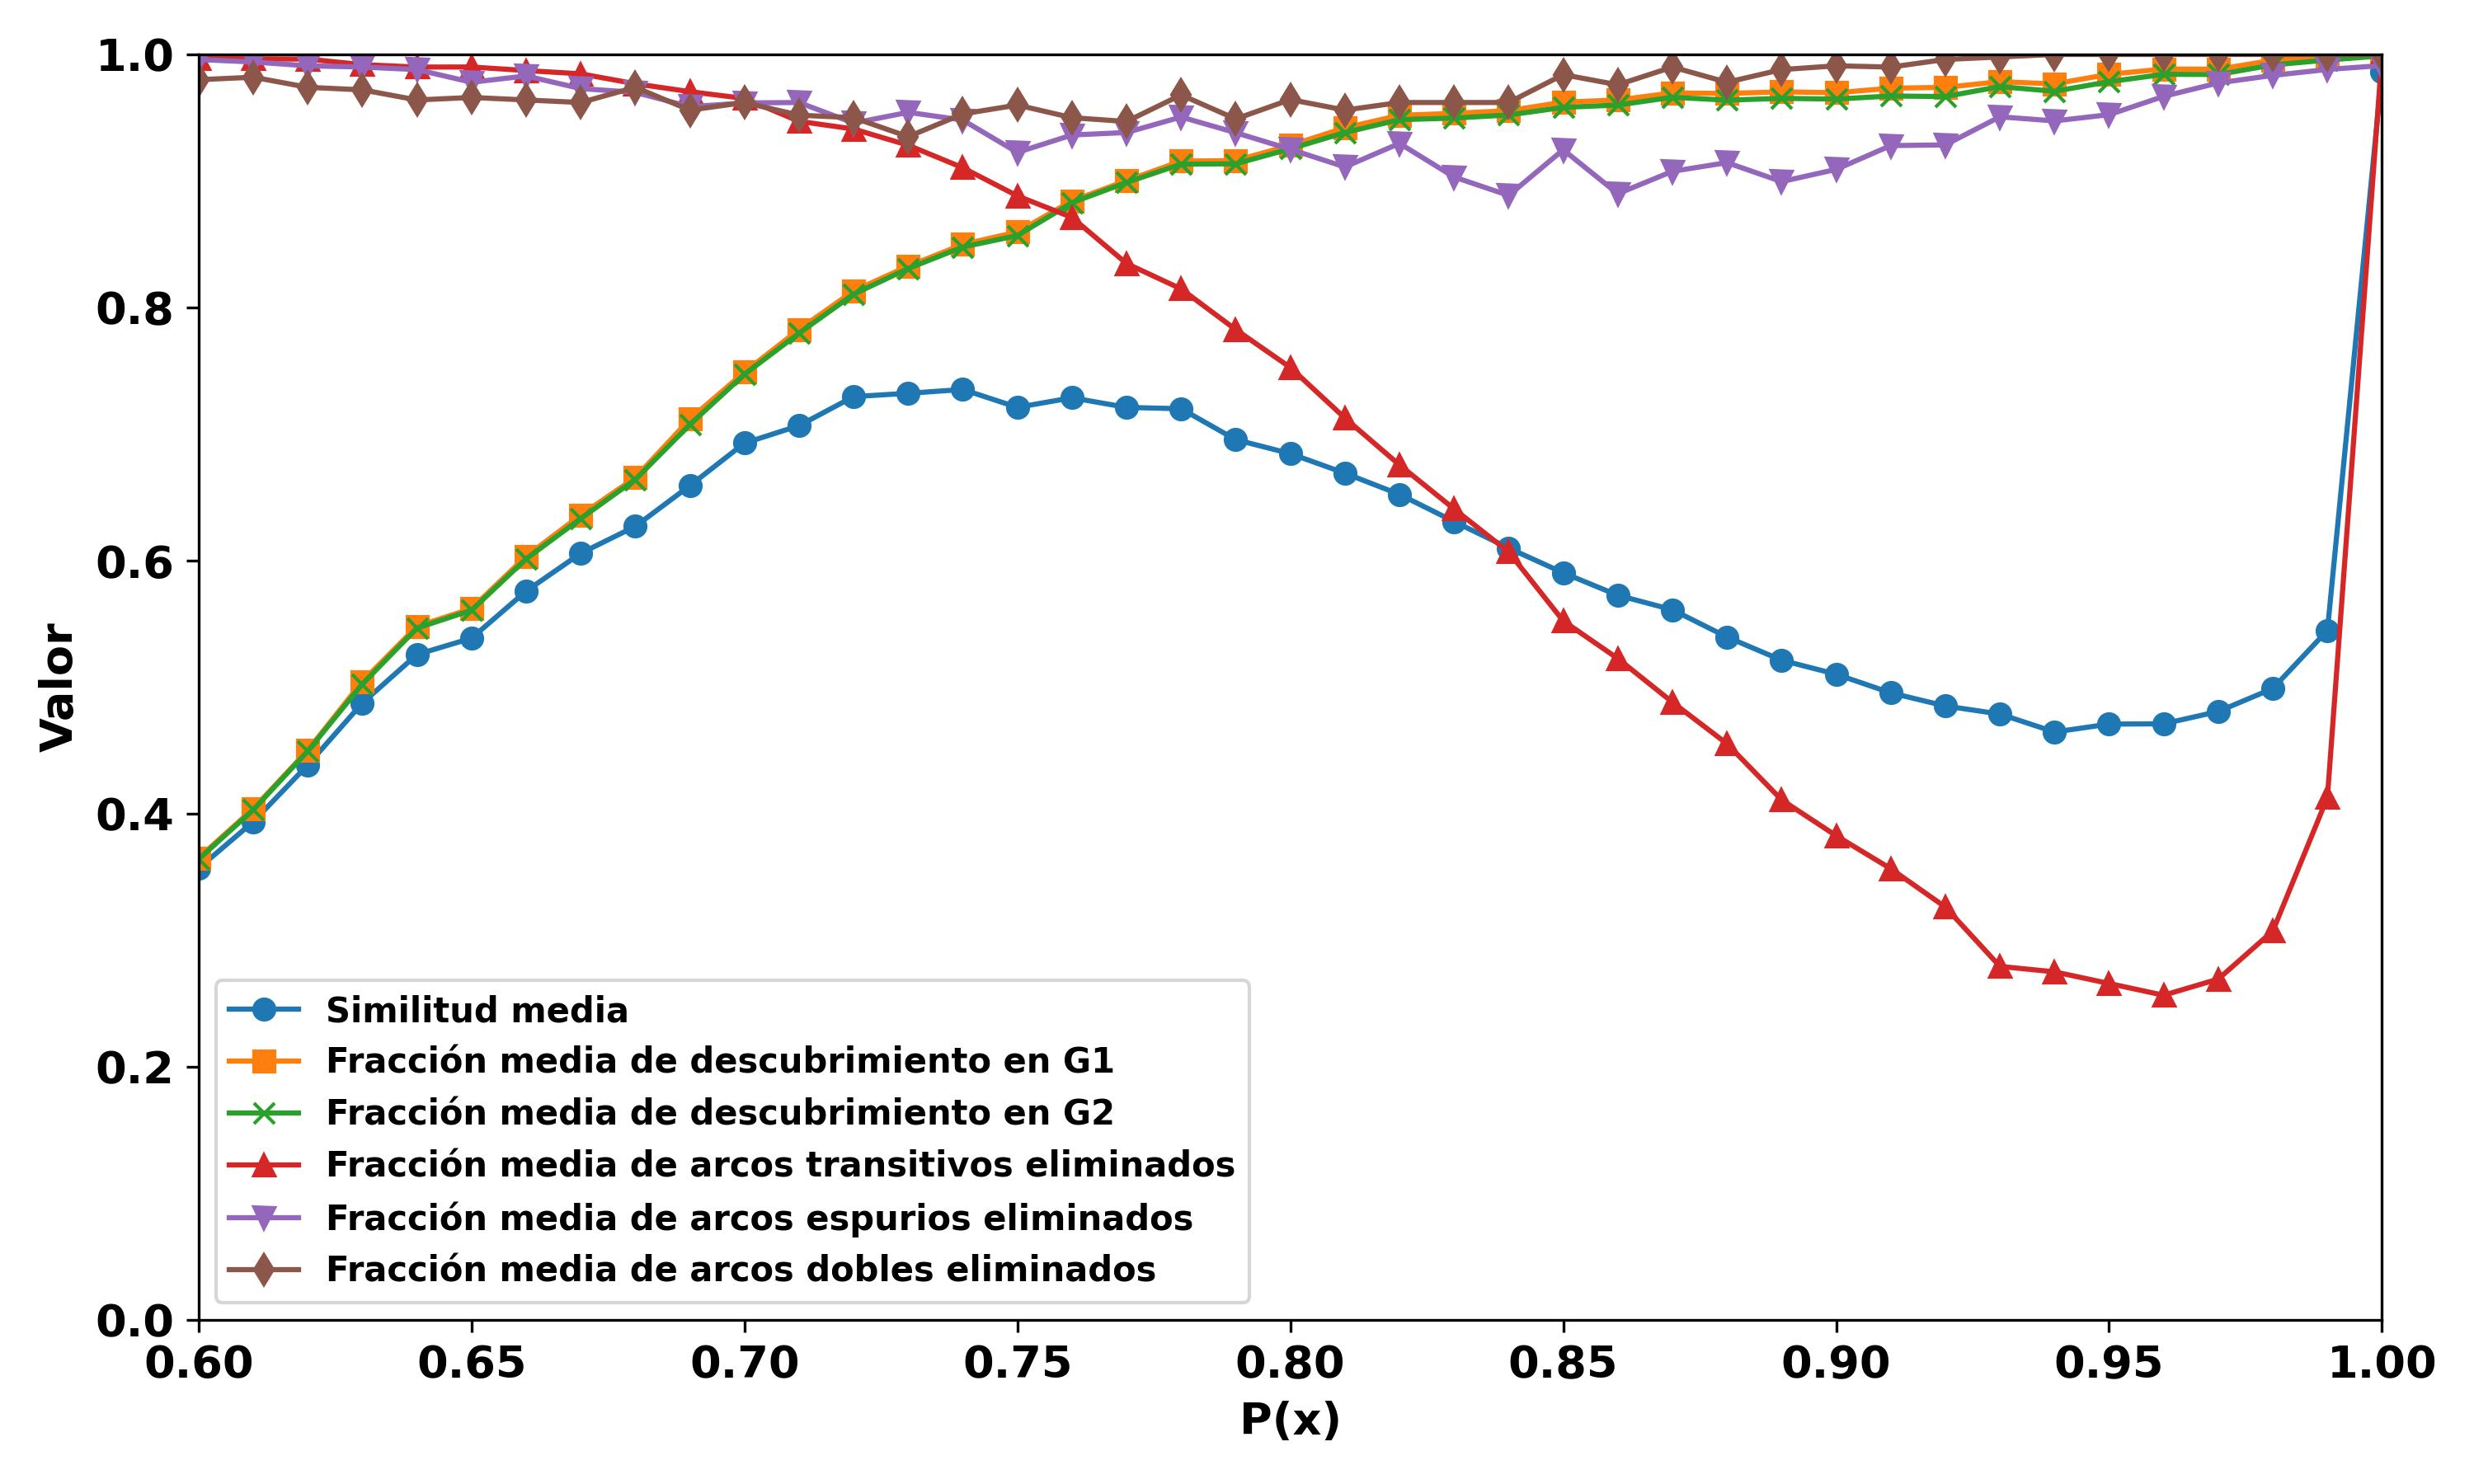
\includegraphics[width=1\textwidth]{tree_x.jpg}
\caption{Performance metrics for each P(X), in 15-vertex trees.}
\label{fig:tree_x}
\end{figure}

\begin{figure}[H]
\centering
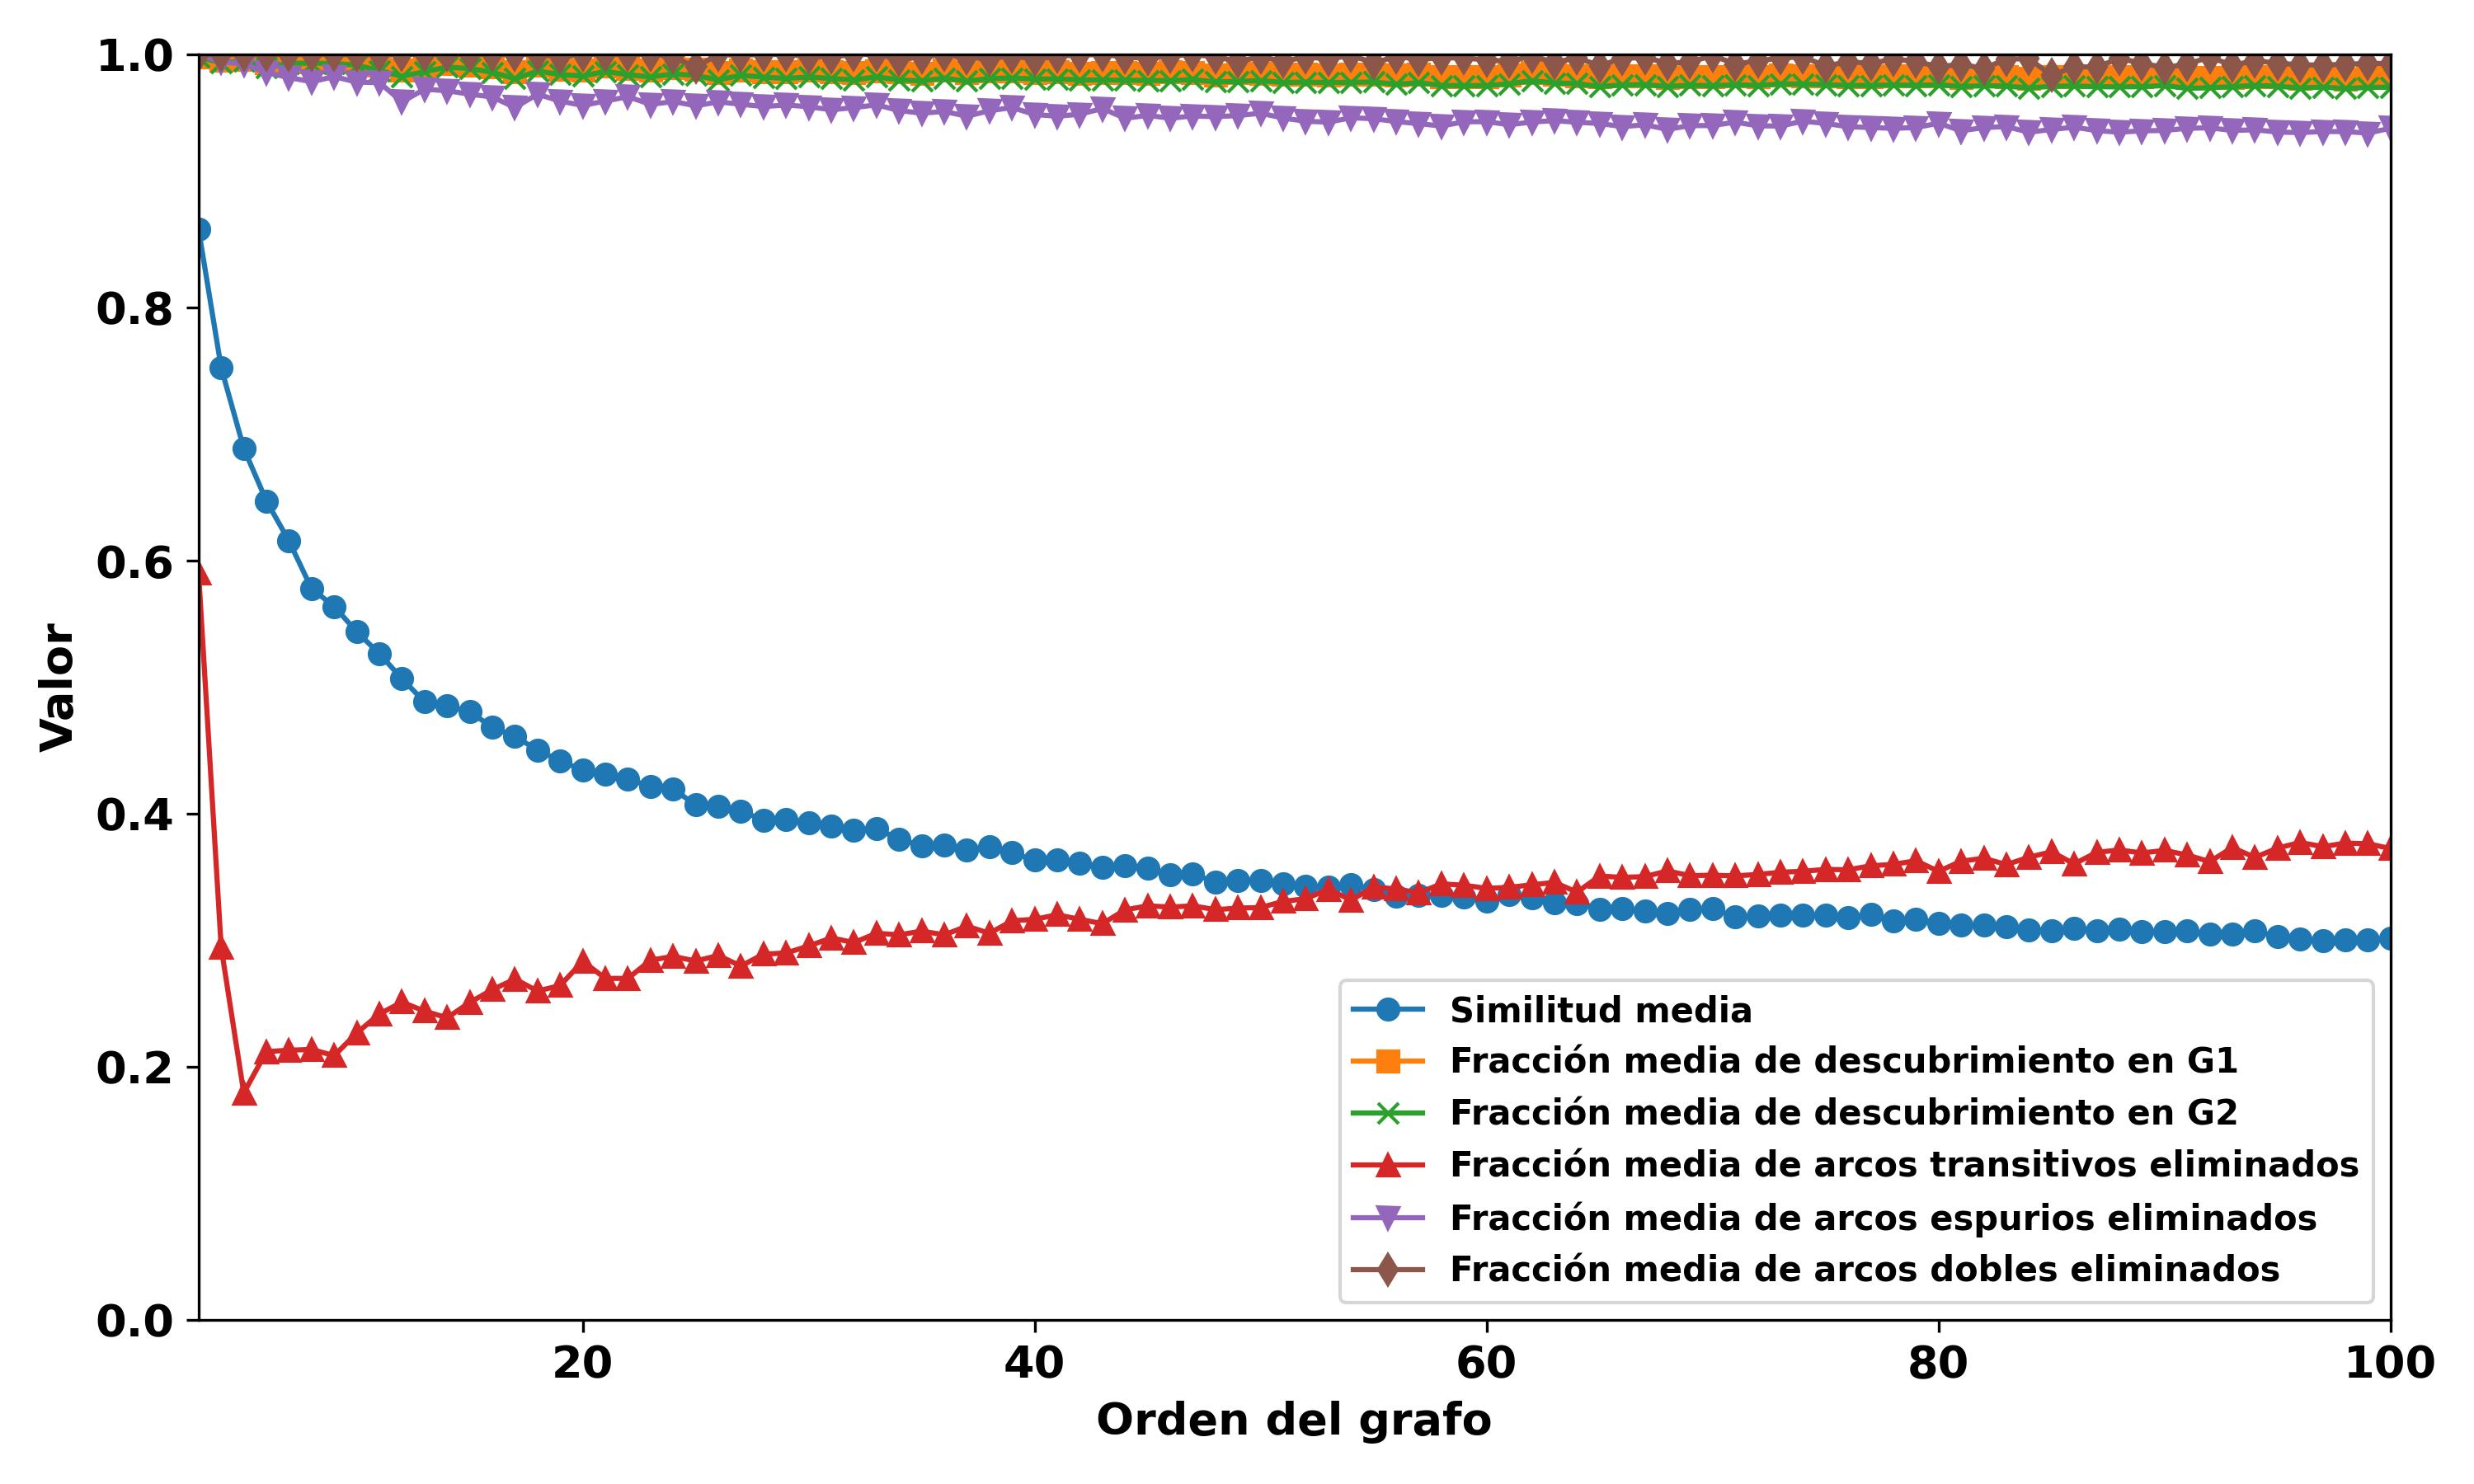
\includegraphics[width=1\textwidth]{tree_n.jpg}
\caption{Performance metrics for each graph order, in trees.}
\label{fig:tree_n}
\end{figure}

\subsubsection{Forests}
Forests, being disjoint collections of trees, introduce multiple connected components. Figure~\ref{fig:forests} shows the behavior of the performance metrics in forests with respect to the number of trees contained in each forest. Each tree in the considered forests is composed of 15 vertices. A decrease in the metrics is observed, ultimately due to the fragmentation of the network into numerous similar disconnected structures.


The fraction most affected by the increase in the number of trees is the elimination of double edges. This situation results from the presence of many vertices with identical structural equations but belonging to different trees. As a result, the number of vertices with equal frequency increases, and when spurious arcs are generated between pairs of these vertices, double edges arise that cannot be oriented according to the robustness criterion. The origin of this ambiguity is that such vertices occupy analogous positions within the structure of their respective trees, as do their parents and children. Consider, for example, an edge $i \leftrightarrow j$, where $i$ and $j$ belong to the same level even though they are in different trees; that is, $i$ and $j$ have the same number of ancestors. Let $i - 1$ and $i + 1$ denote the parent and child of $i$, respectively, and $j - 1$ and $j + 1$ those of $j$. In this context, $i - 1$ and $j - 1$ also belong to the same level, and the same occurs with $i + 1$ and $j + 1$. Recall then that the resampling measures used in the robustness criterion depend on the parent or child most similar to each vertex (see Equations~\ref{eq:rob1} and~\ref{eq:rob2}). However, since these vertices also occupy analogous positions in different trees, the coefficients $H_{iij}$ and $H_{jji}$, on the one hand, and $H_{iijj}$ and $H_{jjii}$, on the other, may be numerically equal with high probability. If, in addition, $H_{iij} > H_0$ and $H_{iijj} > H_0$, then the double arc $i \leftrightarrow j$ cannot be oriented or eliminated through the robustness criterion. As for the decay in the fraction of eliminated spurious arcs, it is due to the fact that, at sufficiently deep levels, arcs may arise between trees that do not correspond to any common parent. Consider that the pairs of vertices ($i$,$j$) and ($k$,$l$) identify parents ($i$ and $k$) and children ($j$,$l$) at the same level in the original forest $G_0$, but corresponding to different trees: ($i$,$j$) belong to tree $T_1$, ($k$,$l$) to tree $T_2$, $i$ has as many ancestors as $k$, and $j$ as many ancestors as $l$. Now suppose that vertex $i$ is located at sufficient depth in the network and therefore has a sufficiently high frequency. It is then possible for a spurious arc $i \rightarrow l$ to be generated in $G_1$, while the real parent of $l$ (that is, $k$) is not connected to $i$. In that case, the spurious arc $i \to j$ could not be eliminated by the Reichenbach test, since there would be no common parent of $i$ and $l$.


The remaining metrics show behavior similar to the case of trees (Figure~\ref{fig:tree_n}). The similarity curve is nearly constant, since it would represent an average of the similarity of each of the trees in the forest. As the number of trees increases, the similarity converges to a limiting value obtained by resampling the case of a single 15-vertex tree. Indeed, the similarity values are close to the value obtained for a single 15-vertex tree (see Figure~\ref{fig:tree_n}). 
\begin{figure}[H]
\centering
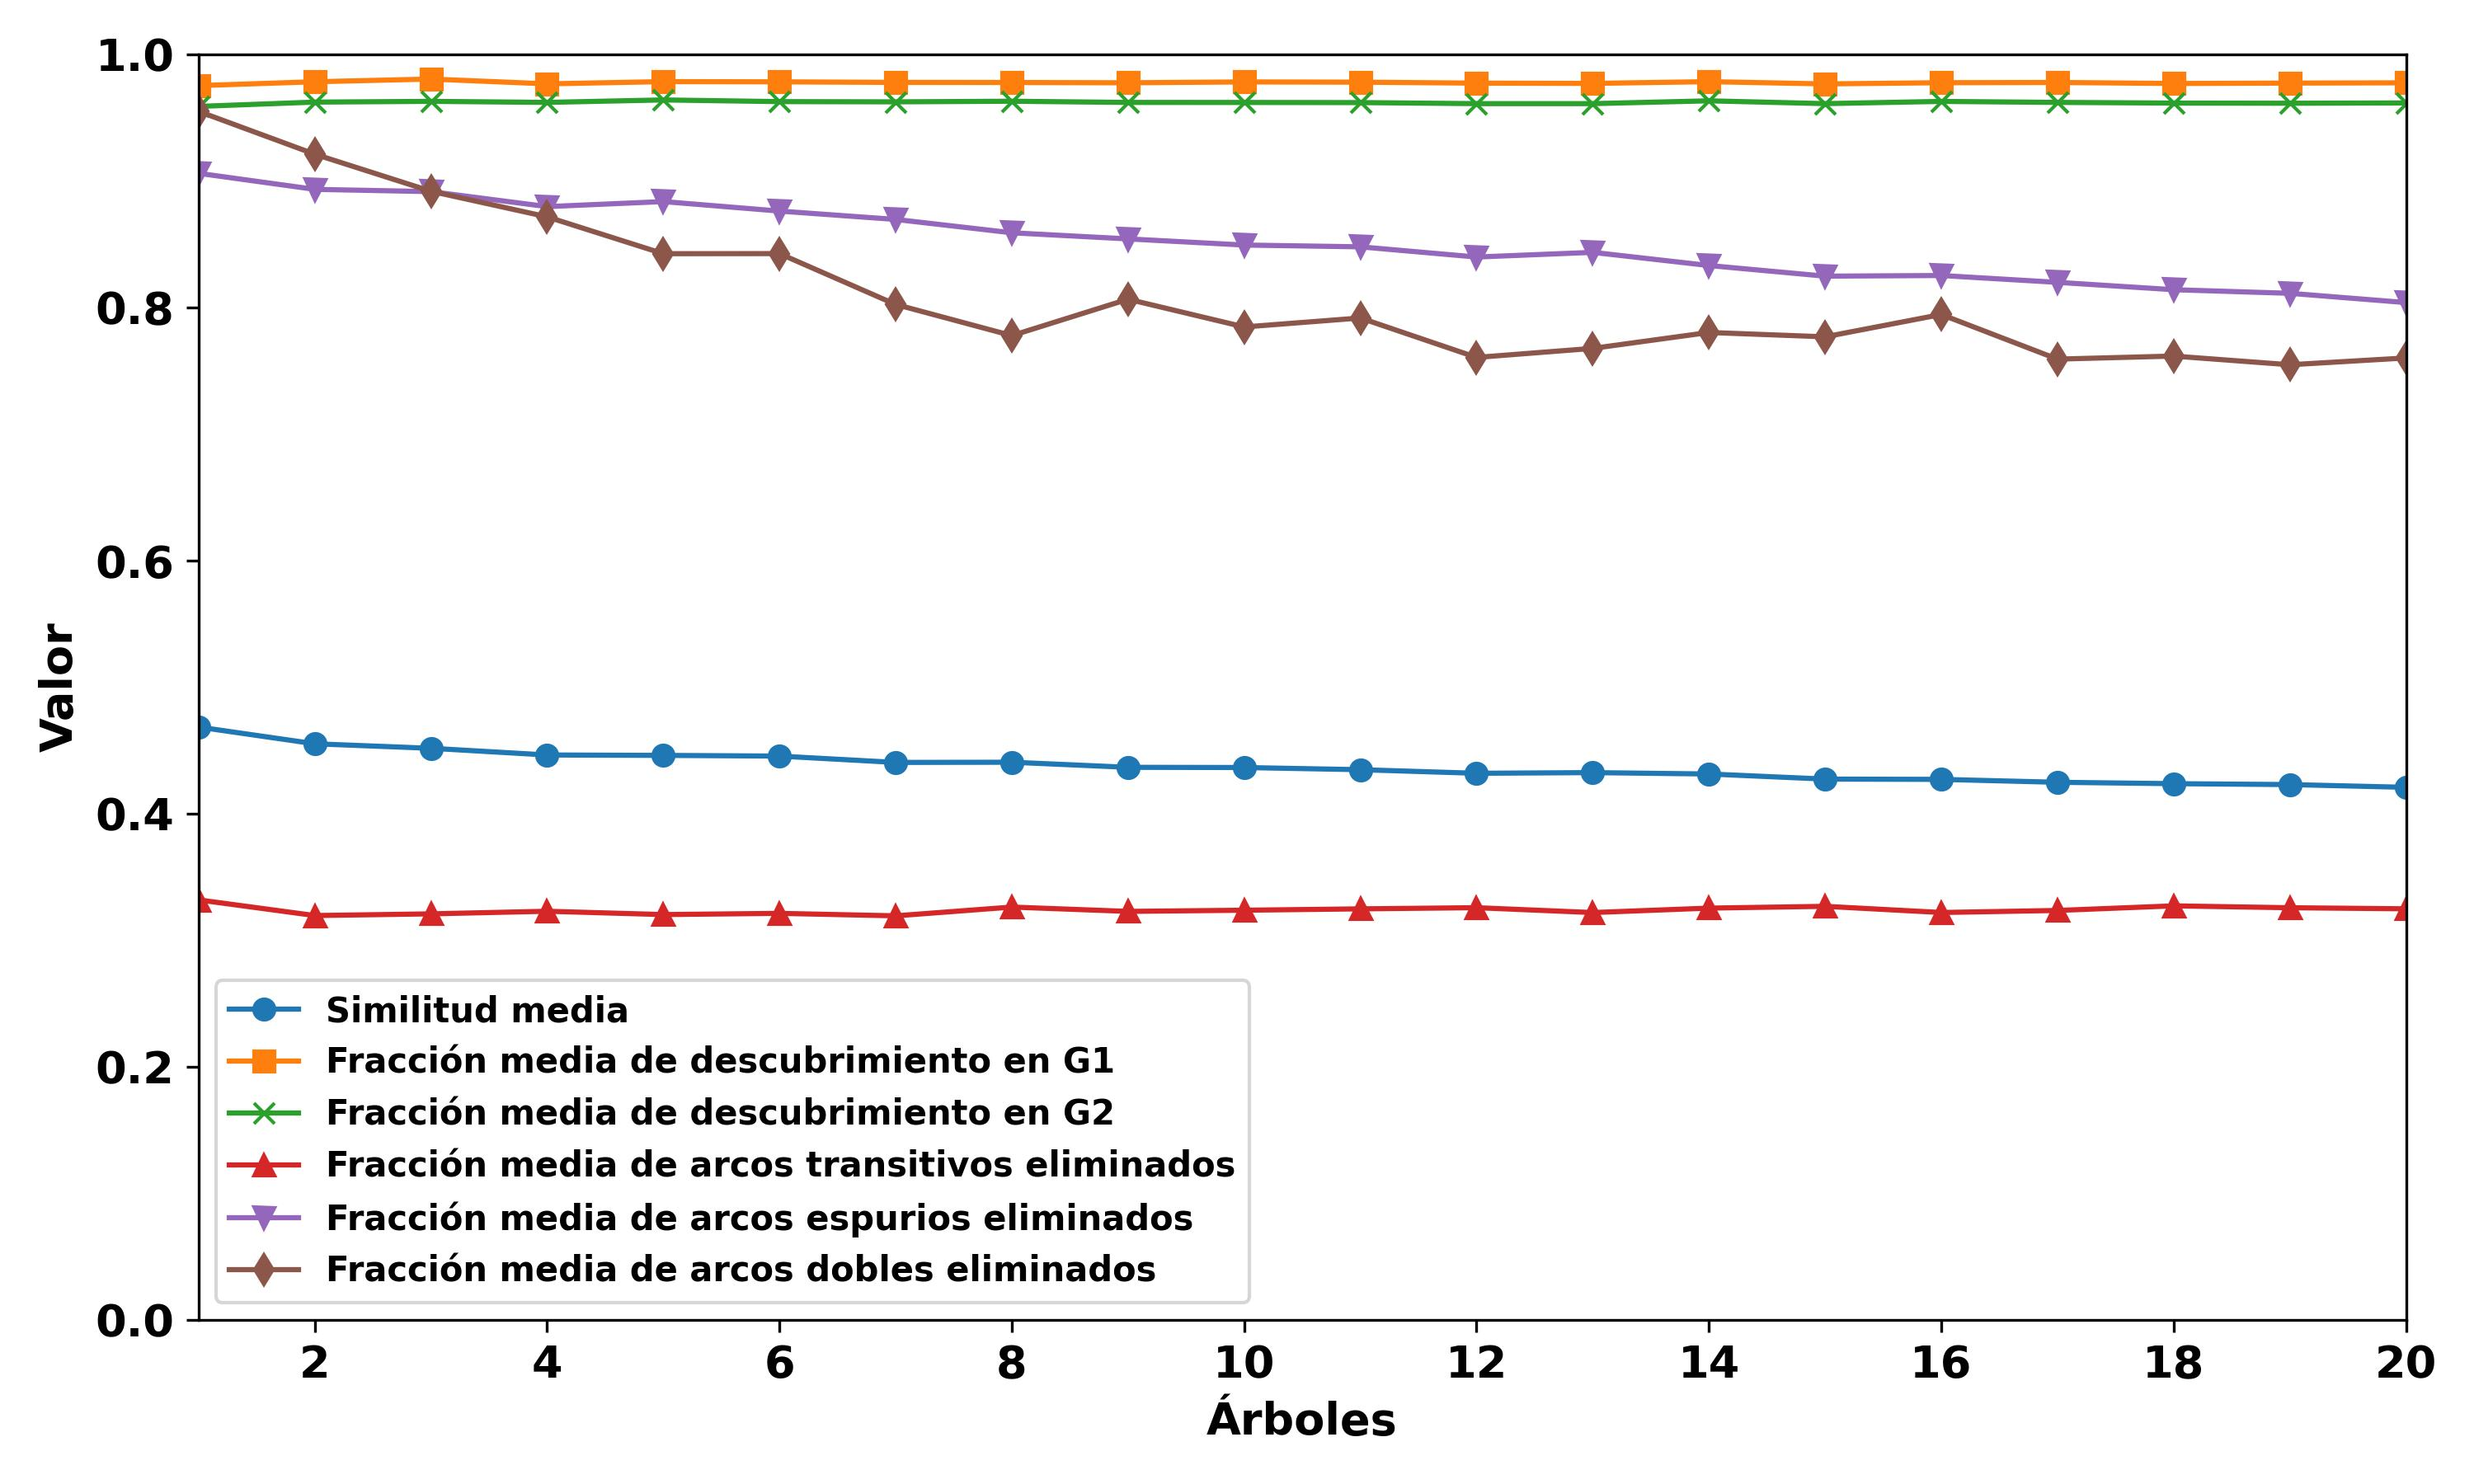
\includegraphics[width=1\textwidth]{forest.jpg}
\caption{Performance metrics for each number of 15-vertex trees, in forests.}
\label{fig:forests}
\end{figure}

\subsubsection{Graphs with immoralities}
The analysis of graphs with immoralities constitutes an essential step toward validating the algorithm in more realistic scenarios. An immorality is a configuration of the type ($i \rightarrow k \leftarrow j$), where vertices $i$ and $j$ act as independent causes of a common vertex $k$, without being connected to each other. This structure makes it possible to model situations in which an effect arises from multiple causal factors that do not necessarily interact with each other, which is characteristic of many complex biological processes. In the graphs treated in this section, there can be no more than one immorality per vertex; additionally, we impose that the vertices containing immoralities have an in-degree equal to 2, whereas in the other vertices the in-degree is no greater than 1.


In this more complex type of graph, the discovery region and the region of non-elimination of real edges must be redefined as functions of the probabilities of the exogenous variables.
For the discovery region, we take as an example the graph i $\rightarrow$ j $\leftarrow$ k. Equations~\ref{eq:pymin} and~\ref{eq:zonedesc} were used, taking $\nu_i$ as the largest frequency among the parent vertices, thereby guaranteeing the joint fulfillment of the discovery conditions for the edges i $\rightarrow$ j and k $\rightarrow$ j; see Equations~\ref{eq:frec} and~\ref{eq:loev}.

To obtain the parameter region $P(X_i)$ and $P(Y_i)$ that guarantees that the Reichenbach test does not eliminate real edges, we use the simple case represented in Figure~\ref{fig:colision1}. In this case, when reconstructing graph $G_1$ prior to the simplification phase, the transitive edge i $ \rightarrow $ k through i $ \rightarrow $ j and j $ \rightarrow $ k is discovered, as represented in Figure~\ref{fig:colision2}. Due to this edge, vertices l and k would have vertex i as a common parent, so the edge l $ \rightarrow $ k represented in Figure~\ref{fig:colision3} is treated by the Reichenbach test. The expressions corresponding to the vertices to be analyzed are:
\begin{align*}
j &= (X_j \land i) \lor Y_j \\
l &= (X_l \land i) \lor Y_l \\
k &= (X_k \land j) \lor (X'_k \land l) \lor Y_k
\end{align*} 
\\
We use Equation~\ref{eq:reichenbach} for the edge l $ \rightarrow $ k with common parent i. For simplicity, developing only the expression conditioned on $\neg i $ we obtain:
\begin{align*}
\nu_{lk}  &= \nu_l P((X_k \land X_j \land i) \lor (X_k \land Y_j) \lor X'_k \lor Y_k) \\
\nu_{lk|\neg i}  &= \nu_{l| \neg i} P((X_k \land Y_j) \lor X'_k \lor Y_k) \\
\nu_{l| \neg i} &= P(Y_l)\\
\nu_{k| \neg i} &= P((X_k \land Y_j) \lor (X'_k \land Y_l) \lor Y_k)
\end{align*}
\\
For convenience, we use the following change of variable:
\begin{equation*}
Z = (X_k \land Y_j) \lor Y_k
\end{equation*}
\\
Substituting these expressions into the conditioned Loevinger coefficient $H_{lk| \neg i}$, we obtain:
\begin{align*}
H_{lk \neg i} &= \frac{P_{lk| \neg i} - P_{l| \neg i} P_{k| \neg i}}{P_{l| \neg i} (1 - P_{k| \neg i})} \\
H_{lk \neg i} &= \frac{P_{l| \neg i} P(Z \lor X'_k) - P_{l| \neg i} P_{k| \neg i}}{P_{l| \neg i} (1 - P_{k| \neg i})} \\
H_{lk \neg i} &= \frac{P(Z \lor X'_k) - P_{k| \neg i}}{(1 - P_{k| \neg i})} \\
H_{lk \neg i} &= \frac{P(X'_k)(1 - P(Z)) - P(X'_k)P(Y_l)(1 - P(Z))}{(1 - P(Z)) - P(X'_k)P(Y_l)(1 - P(Z))} \\
H_{lk \neg i} &= \frac{P(X'_k) - P(X'_k) P(Y_l)}{1 - P(X'_k) P(Y_l)}
\end{align*}
\\
Now, imposing the condition $H_{lk| \neg i} > H_0$ with $H_0 = 0.5$ to preserve the edge l $\rightarrow$ k requires:
\begin{equation}
\label{eq:incheck}
P(X'_k) > \frac{1}{2-P(Y_l)}
\end{equation}
\\
Equation~\ref{eq:incheck} represents the region where Reichenbach does not eliminate the real arc in this case. Note that this expression is similar to that obtained in Equation~\ref{eq:region}. However, there are more complex cases in which the path from vertex i to vertex k is mediated by a larger number of vertices. These more general cases require greater attention and are not developed in this work.


\begin{figure}[h!]
\centering
\begin{subfigure}[b]{0.25\textwidth}
	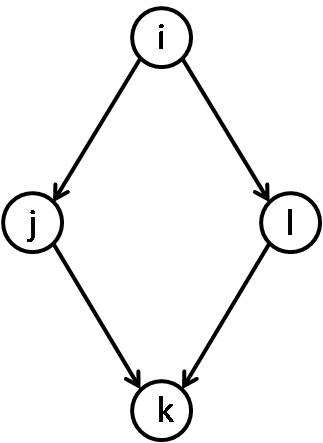
\includegraphics[width=\textwidth]{colision1.jpg}
	\caption{}
	\label{fig:colision1}
	\end{subfigure}
	\hfill
\begin{subfigure}[b]{0.25\textwidth}
	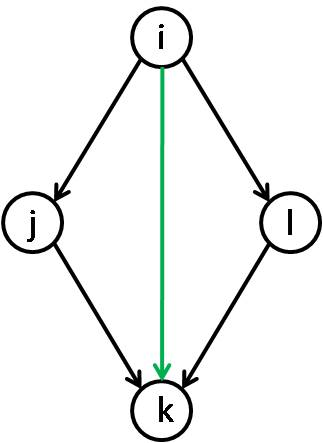
\includegraphics[width=\textwidth]{colision2.jpg}
	\caption{}
	\label{fig:colision2}
	\end{subfigure}
	\hfill
\begin{subfigure}[b]{0.25\textwidth}
	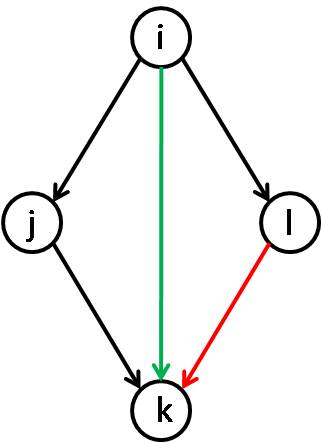
\includegraphics[width=\textwidth]{colision3.jpg}
	\caption{}
	\label{fig:colision3}
	
\end{subfigure}
\hfill

\caption{Representation of a DAG, its transitive edge (through i $ \rightarrow $ j and j $ \rightarrow $ k), and the edge to be analyzed by the Reichenbach test, represented in green and red, respectively.}
\label{fig:colisiones}
\end{figure}

In Figure~\ref{fig:inmorality}, the performance metrics are represented as a function of the number of immoralities in the graph, while keeping the number of vertices constant and equal to 100, in order not to compromise the variation of the metrics due to graph order. As the number of immoralities increases, the difference between the discovery fractions increases slightly, indicating the elimination of real arcs in the simplification phase. There are possible configurations within this type of graph, similar to those treated to prevent the Reichenbach and Mokken tests from eliminating real arcs, that have not been previously analyzed and may give rise to cases of real-edge elimination. A first case occurs when one of the edges forming an immorality is the first leg of a triangle, and its hypotenuse is a transitive edge; see Figure~\ref{fig:inn}. Another specific case occurs when a spurious edge is constructed and, together with an edge that forms an immorality, gives rise to the elimination shown in Figure~\ref{fig:imm}. However, the discovery fraction in the inferred graph remains high.

\begin{figure}[h!]
\centering
\begin{subfigure}[b]{0.3\textwidth}
	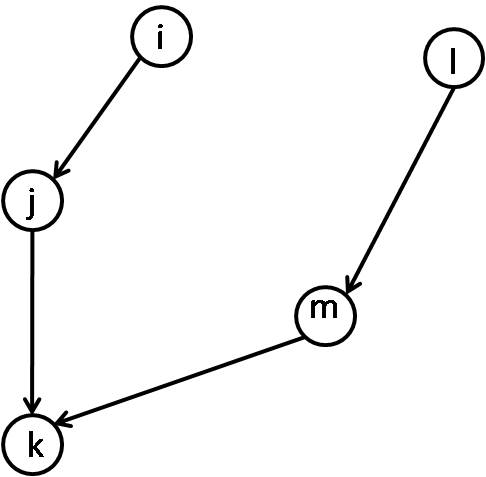
\includegraphics[width=\textwidth]{imm1.jpg}
	\caption{}
	\label{fig:imm1}
	\end{subfigure}
	\hfill
\begin{subfigure}[b]{0.3\textwidth}
	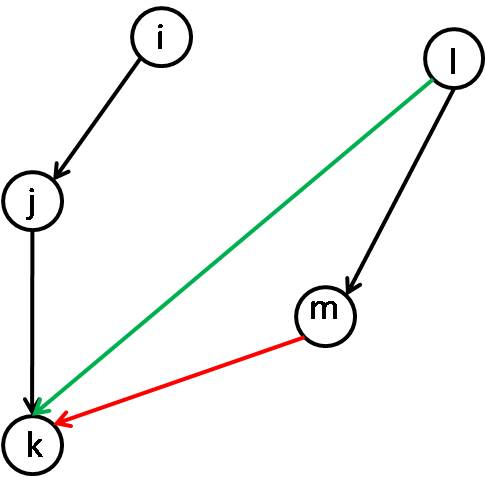
\includegraphics[width=\textwidth]{imm2.jpg}
	\caption{}
	\label{fig:imm2}
	\end{subfigure}
	\hfill
\begin{subfigure}[b]{0.3\textwidth}
	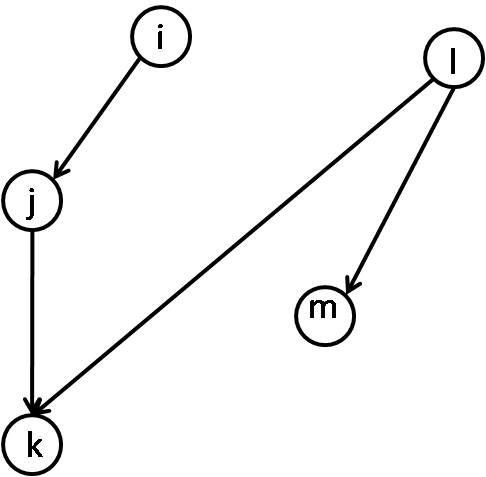
\includegraphics[width=\textwidth]{imm3.jpg}
	\caption{}
	\label{fig:imm3}
	
\end{subfigure}
\hfill

\caption{Example of reconstruction of a graph with an immorality. The inference of a transitive edge (green edge) causes a real edge to be treated as spurious (red edge) and eliminated by the Reichenbach test.}
\label{fig:inn}
\end{figure}



\begin{figure}[h!]
\centering
\begin{subfigure}[b]{0.3\textwidth}
	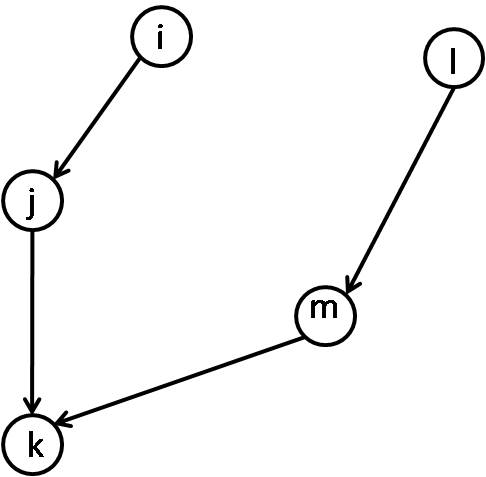
\includegraphics[width=\textwidth]{imm1.jpg}
	\caption{}
	\label{fig:inn1}
	\end{subfigure}
	\hfill
\begin{subfigure}[b]{0.3\textwidth}
	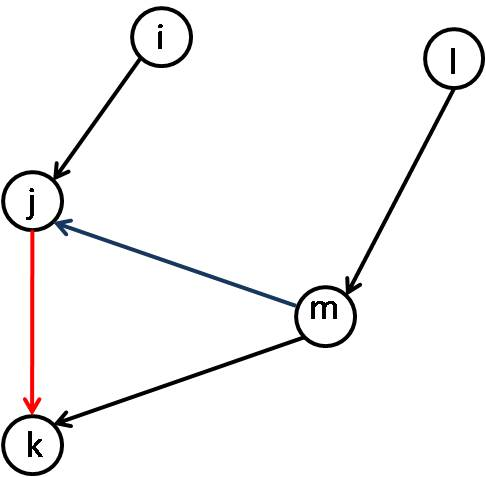
\includegraphics[width=\textwidth]{inn2.jpg}
	\caption{}
	\label{fig:inn2}
	\end{subfigure}
	\hfill
\begin{subfigure}[b]{0.3\textwidth}
	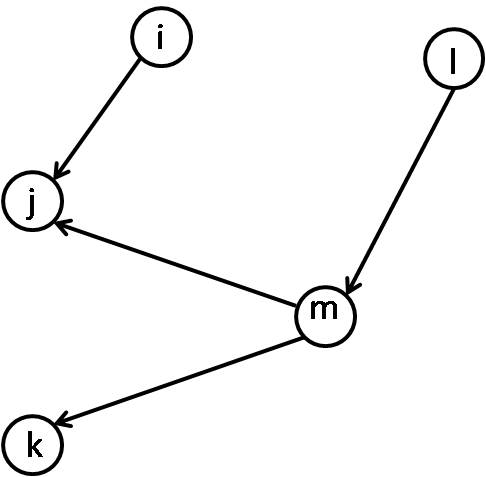
\includegraphics[width=\textwidth]{inn3.jpg}
	\caption{}
	\label{fig:inn3}
	
\end{subfigure}
\hfill

\caption{Example of reconstruction of a graph with an immorality. The construction of a spurious edge (blue edge) causes a real edge to be treated as spurious (red edge) and eliminated by the Reichenbach test.}
\label{fig:imm}
\end{figure}


To visualize the performance of the algorithm in reconstructing more complex graphs, Figure~\ref{fig:DAG} shows the performance metrics as a function of graph order for DAGs. In this type of graph, cases may arise in which, in the original graph, real edges are also transitive edges and are eliminated by the Mokken test; see Figure~\ref{fig:mokk}. Addressing this type of case, as well as a detailed analysis of other possible problematic cases in DAGs, is not an objective of this work; the aim is only to generally validate the operation of \texttt{CChains} in different classes of graphs.


\begin{figure}[H]
\centering
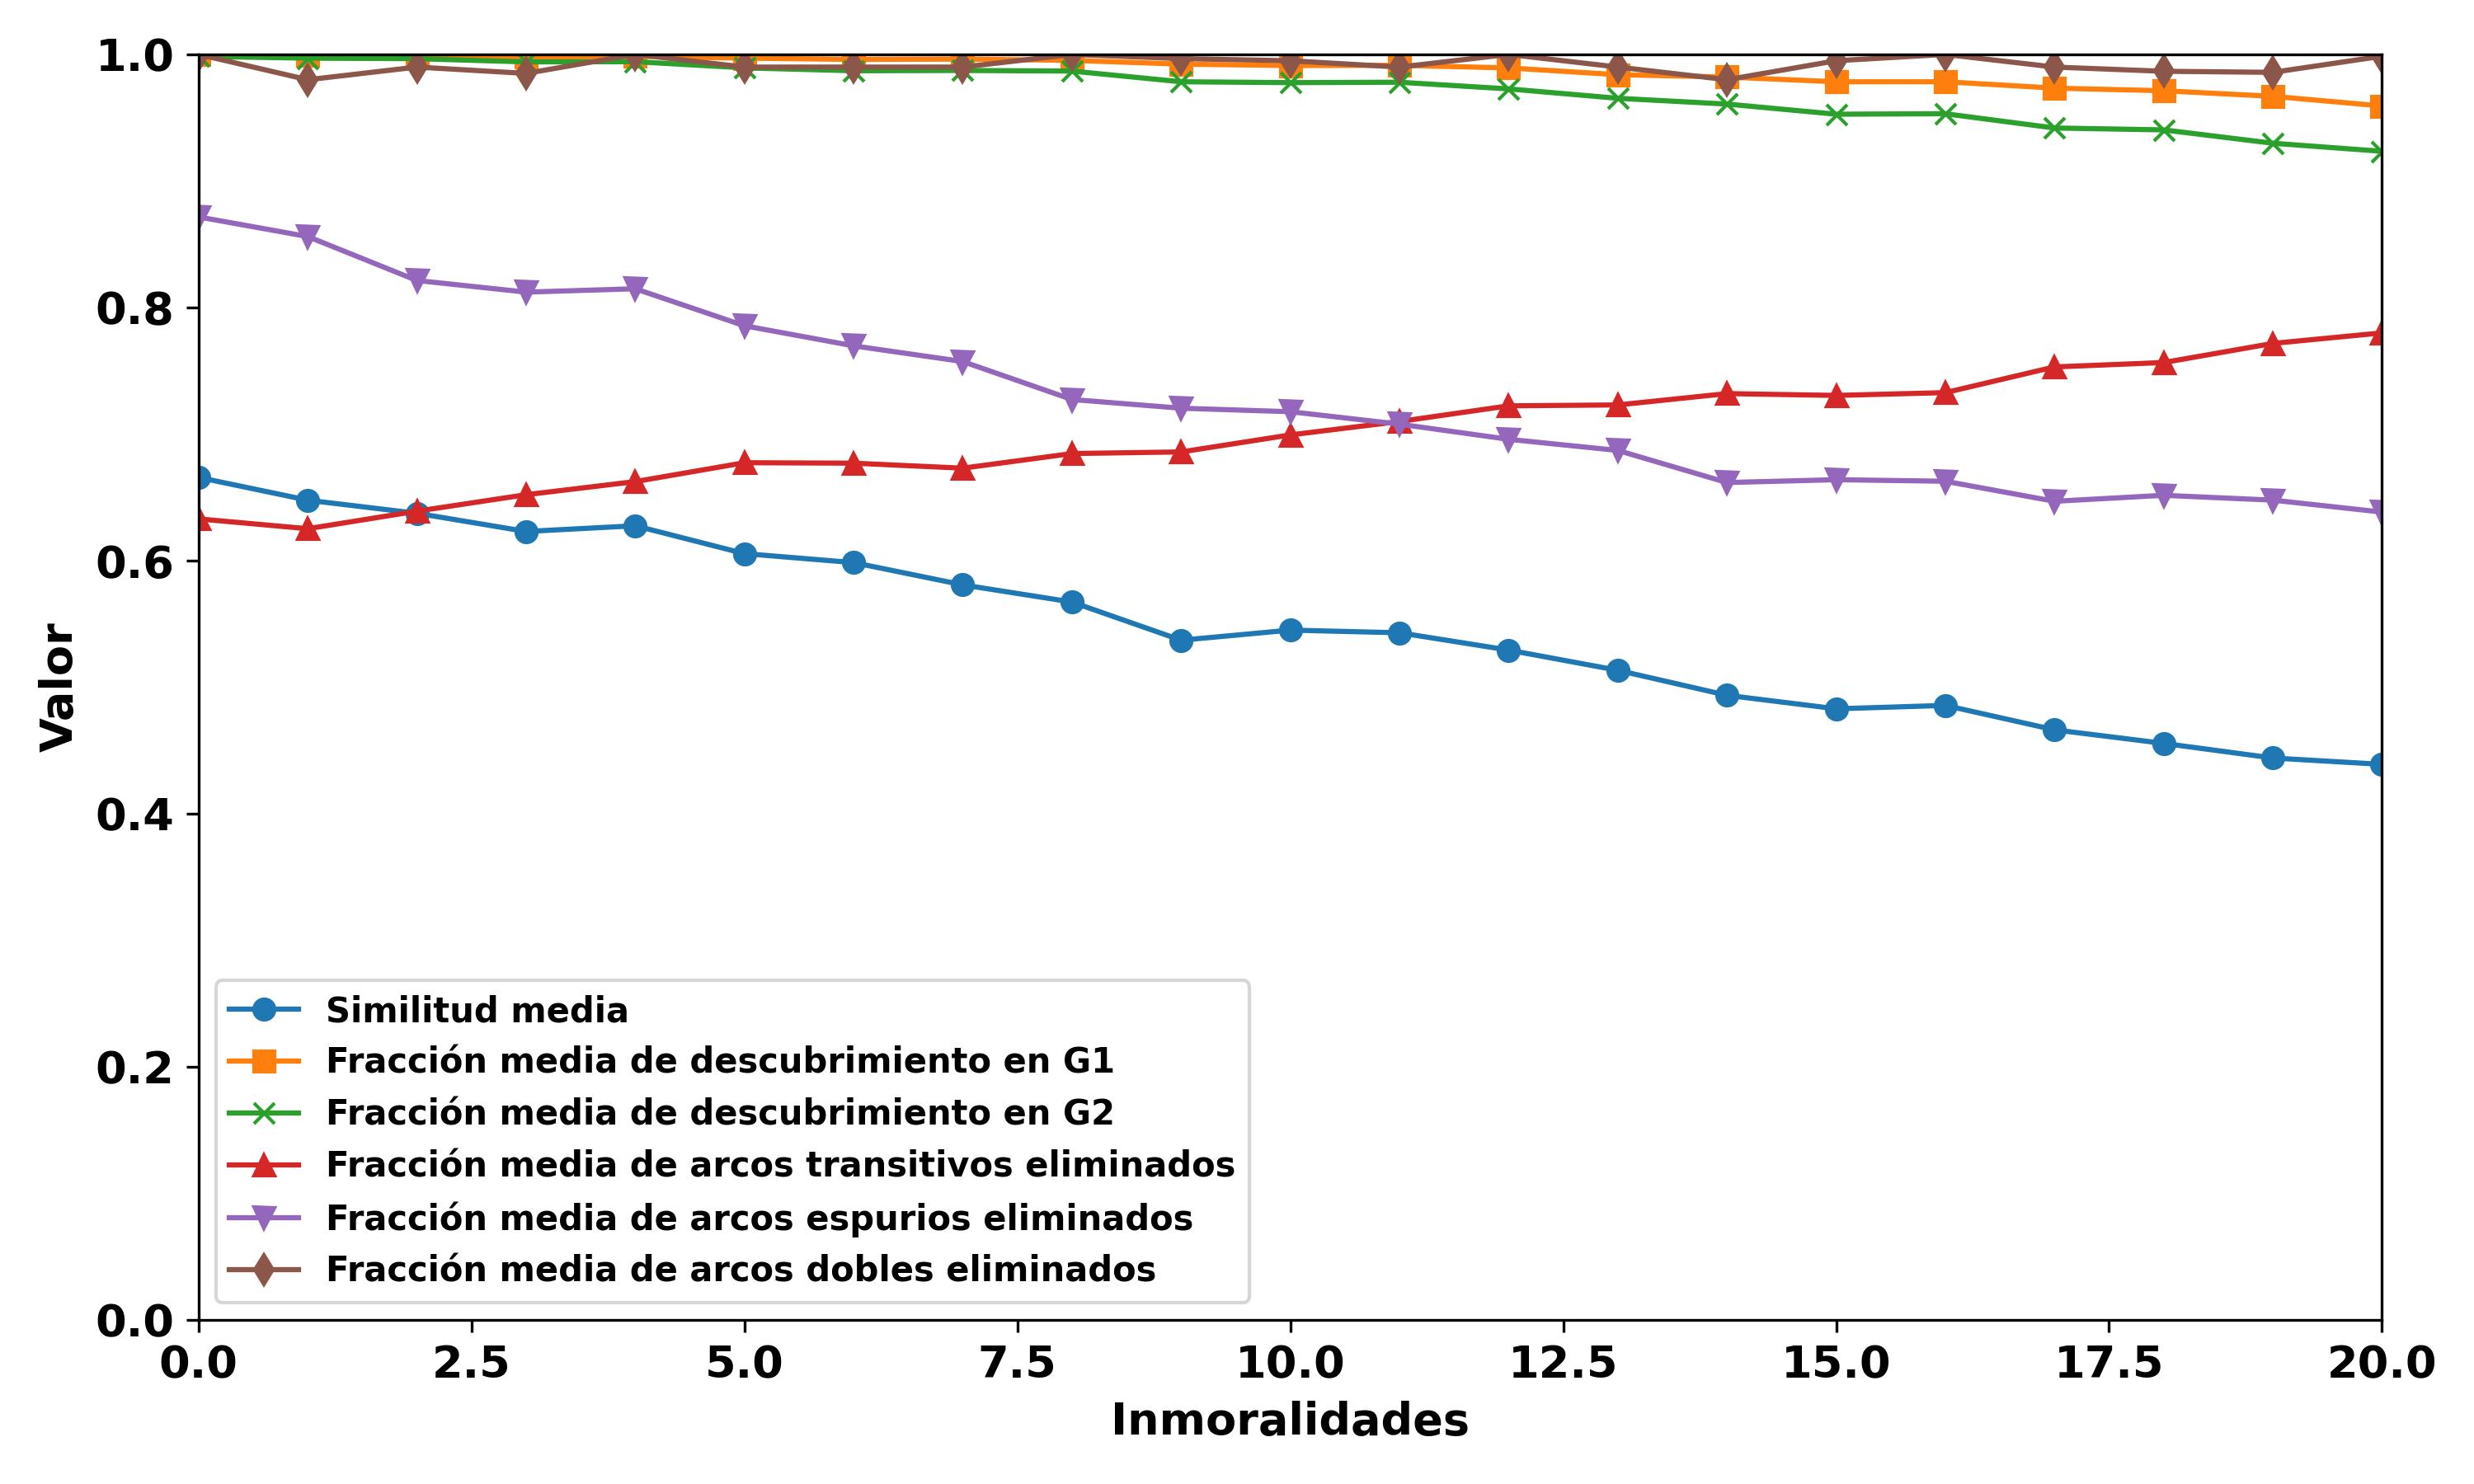
\includegraphics[width=1\textwidth]{inmorality.jpg}
\caption{Performance metrics for each number of immoralities.}
\label{fig:inmorality}
\end{figure}

\begin{figure}[H]
\centering
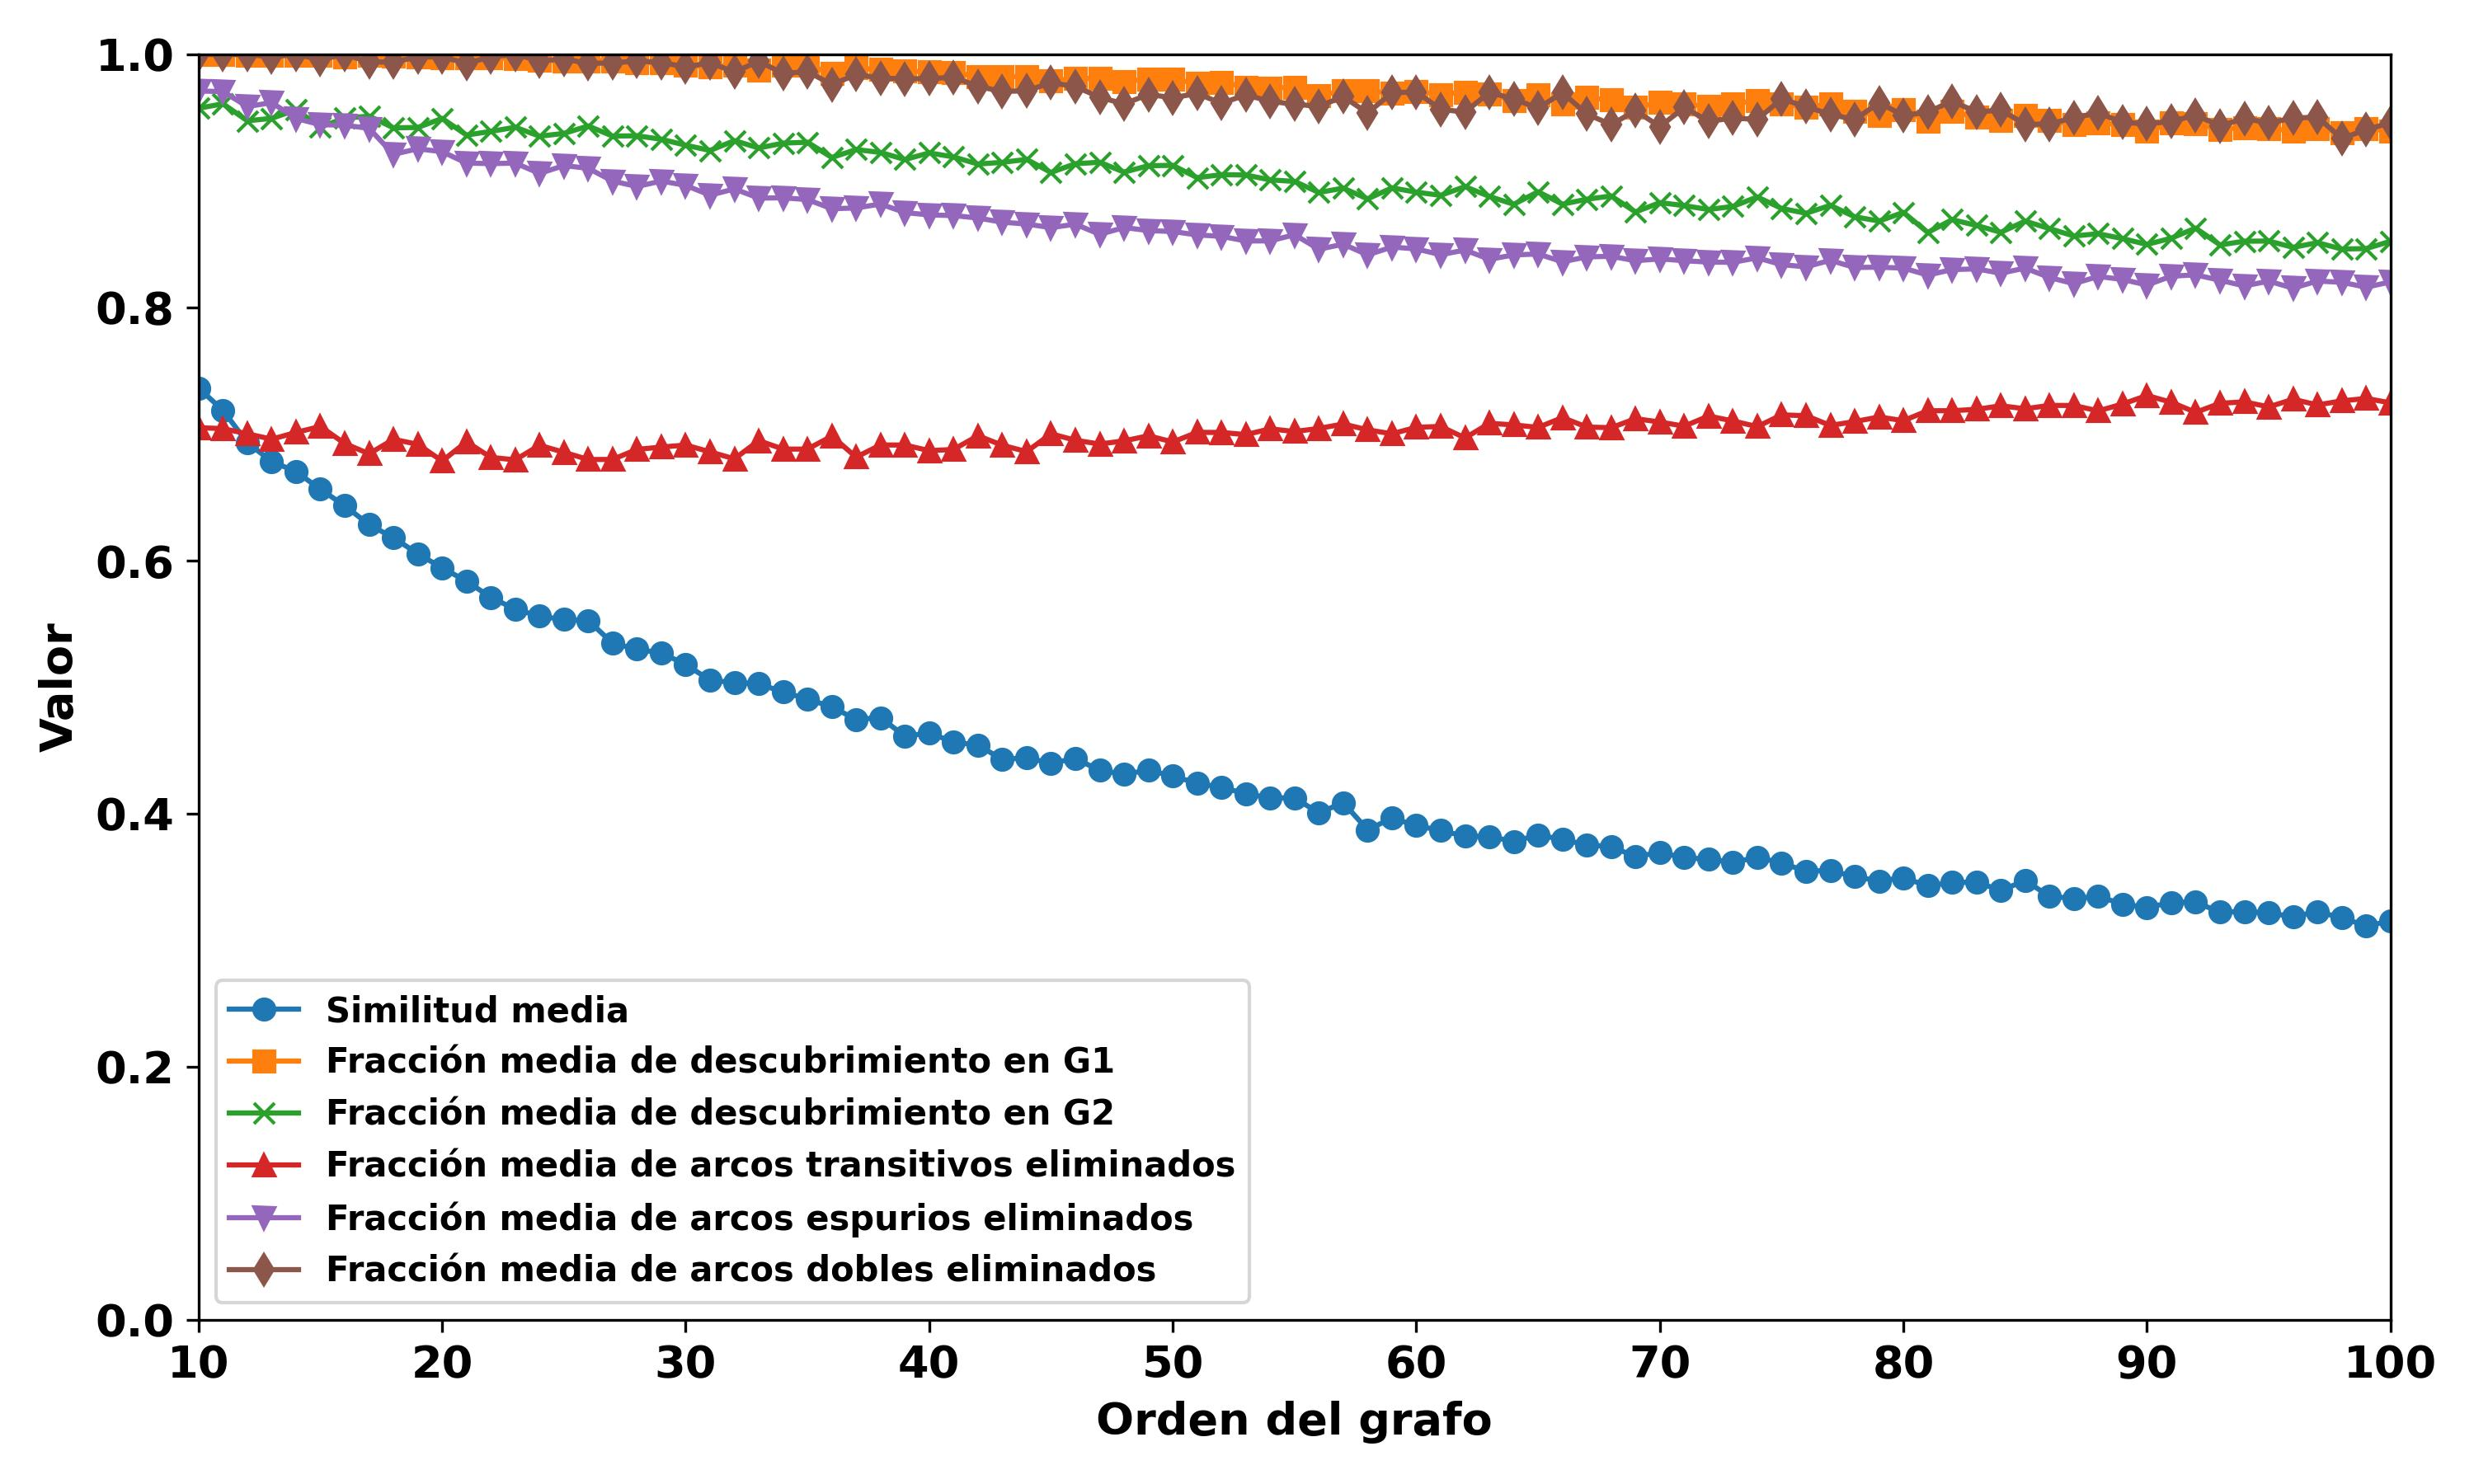
\includegraphics[width=1\textwidth]{DAG_analysis.jpg}
\caption{Performance metrics for each graph order, in DAGs.}
\label{fig:DAG}
\end{figure}

\begin{figure}[h!]
\centering
\begin{subfigure}[b]{0.28\textwidth}
	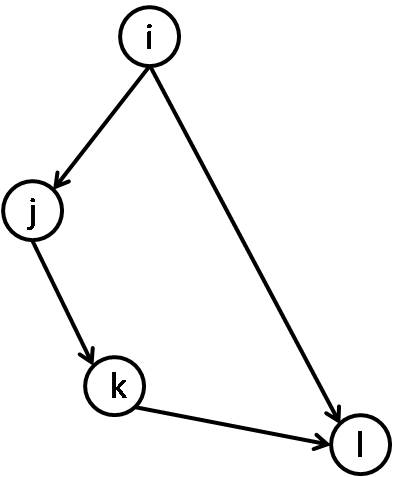
\includegraphics[width=\textwidth]{mokk1.jpg}
	\caption{}
	\label{fig:mokk1}
	\end{subfigure}
	\hfill
\begin{subfigure}[b]{0.28\textwidth}
	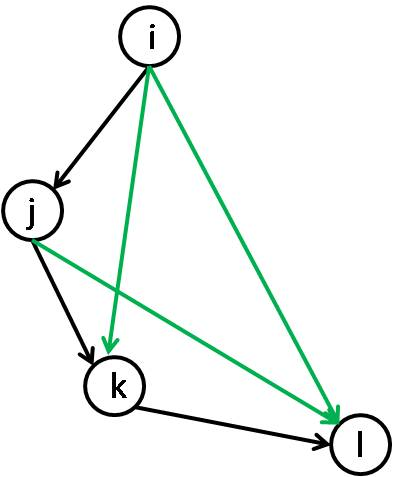
\includegraphics[width=\textwidth]{mokk2.jpg}
	\caption{}
	\label{fig:mokk2}
	\end{subfigure}
	\hfill
\begin{subfigure}[b]{0.28\textwidth}
	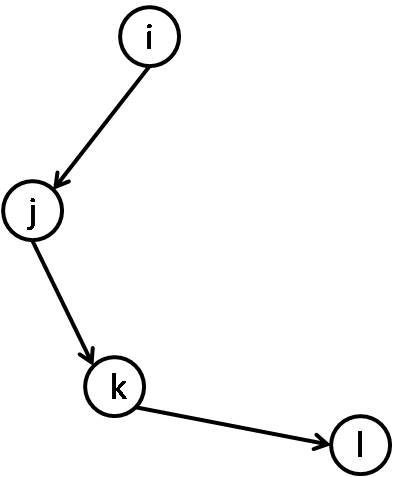
\includegraphics[width=\textwidth]{mokk3.jpg}
	\caption{}
	\label{fig:mokk3}
	
\end{subfigure}
\hfill

\caption{Representation of a DAG with a real transitive edge eliminated by the Mokken test.}
\label{fig:mokk}
\end{figure}


\subsection*{Summary of results on synthetic data}

The tests performed on synthetic data made it possible to systematically and quantitatively evaluate the effectiveness of the implemented causal discovery method. The analysis of the recovery fractions, together with the fractions of eliminated spurious, double, and transitive edges, provided a solid set of metrics for judging the performance of the algorithm.

It was observed that, for all types of graphs considered---including chains, trees, forests, and structures with immoralities---the discovery fractions were consistently high. This behavior constitutes sufficient evidence to conclude that the method is capable of identifying true causal relationships with an acceptable level of precision, even under conditions of increasing complexity.

Regarding the graph-similarity metric, although its values were not particularly high in all cases, it should be noted that this reduction was due exclusively to the presence of non-eliminated transitive edges in the inferred graph. As previously discussed, these edges do not represent false causal relationships, but rather legitimate structural redundancies that, although they do not alter causal validity, increase the complexity of the resulting graph. Therefore, similarity must be interpreted with caution, taking this aspect into account.

Finally, this validation process made it possible not only to verify the efficiency of the method, but also to clarify the conditions under which it is reliable. In particular, it has highlighted that causal inference is based on implicit hypotheses about the exogenous variables and their probabilistic behavior. It has been shown that, under reasonable conditions---such as the ordered distribution of frequencies and the proper choice of noise parameters---the algorithm produces coherent results, which reinforces its applicability in real contexts.

Overall, this validation has served as sufficient evidence of the robustness of the proposed approach and has provided a useful interpretive framework for extending it to networks obtained from real gene expression data, which will be addressed in the following sections.



\section{Application to real cancer data}
\label{sec:3.3}


\subsection{Description of the real RNASeq data}

The data used come from \textit{The Cancer Genome Atlas} (TCGA) repository, which contains gene expression profiles corresponding to primary tumor samples and normal tissues. In particular, data corresponding to three tissue types were used: prostate adenocarcinoma (PRAD), lung adenocarcinoma (LUAD), and lung squamous cell carcinoma (LUSC). Each of these tissues can give rise to solid tumors, and the available expression profiles belong to patients who suffer from them. Nevertheless, the TCGA data contain both normal and tumor clinical samples, with a bias in favor of cancer samples. The samples were classified using histopathological techniques, and gene expression levels were obtained using RNA sequencing (\textit{RNA-Seq}). Gene expression was quantified in terms of \textit{Fragments Per Kilobase of transcript per Million mapped reads} (FPKM), a normalized measure that allows the relative abundance of transcripts to be compared across genes and samples\cite{biomarkers}.

\subsection{Data preprocessing}
\label{sec:prepro}

Gene expression data obtained by RNA-Seq exhibit a strongly skewed distribution, with a large number of low-frequency outliers. Therefore, it is more appropriate to use the geometric mean, rather than the arithmetic mean, as a representative measure of the expression level of a gene.

The RNA-Seq technique is not precise for detecting very low expression levels, and may record spurious null values in genes that are nearly silenced. To mitigate this effect and allow the use of the geometric mean, a small uniform offset of \(0.1\) FPKM is applied to all expression values; this does not significantly affect the interpretation of the results\cite{biomarkers}.

Let \( e_{gs} \) be the expression level of gene \( g \) in sample \( s \) after the aforementioned offset. For each tissue, a reference value \( e_g^{(\text{ref})} \) is estimated, calculated as the geometric mean of \( e_{gs} \) over all normal samples \( s \in N \), where \( N \) is the set of normal samples\cite{biomarkers}:
\begin{equation}
e_g^{(\text{ref})} = \left( \prod_{s \in N} e_{gs} \right)^{1/|N|}
\end{equation}
\\
Next, the relative change in expression (\textit{fold change}) is calculated for each sample using the base-2 logarithm of the ratio between the observed expression and the reference value:
\begin{equation}
\hat{e}_{gs} = \log_2 \left( \frac{e_{gs}}{e_g^{(\text{ref})}} \right)
\end{equation}
\\
This transformation makes it possible to treat overexpression (\( \hat{e}_{gs} < -1 \)) and underexpression (\( \hat{e}_{gs} > -1 \)) of a gene symmetrically. The value of \( \hat{e}_{gs} \) is then discretized, considering that the expression of a gene \( g \) is altered in a sample \( s \) if:
\begin{equation}
|\hat{e}_{gs}| > 1
\end{equation}


In this way, a binary matrix \( M \) is constructed, where each element \( m_{gs} \) takes the value 1 if the expression of gene \( g \) is altered in sample \( s \), and 0 otherwise:
\begin{equation}
m_{gs} = 
\begin{cases}
1 & \text{si } |\hat{e}_{gs}| > 1 \\\\
0 & \text{si } |\hat{e}_{gs}| \leq 1
\end{cases}
\end{equation}
\\
The matrix \( M \) thus obtained represents the pattern of gene-expression alterations across the set of samples and constitutes the input of the algorithm implemented in \texttt{CChains} for the inference of the gene deregulation causal network.


\subsection{Construction of the gene expression causal network}
This section addresses the application of the causal discovery algorithm implemented in the \texttt{CChains} code using gene expression profiles obtained from \textit{The Cancer Genome Atlas} (TCGA) repository for the tissue types considered. The objective of this stage is to infer gene deregulation networks from binarized \textit{RNA-Seq} data (see Section~\ref{sec:prepro}). For each tissue, a directed causal network is generated in which the vertices represent genes and the edges represent possible causal quasi-sufficiency relationships between their deregulations. The construction of these networks makes it possible to explore the causal architecture of gene deregulation in different cancer types and provides a compact representation of molecular mechanisms that may be relevant in carcinogenesis.
Table~\ref{tab:metrics} summarizes some general characteristics of the networks obtained for the three tissues explored.

\begin{table}[H]
\centering
\caption{Global network metrics calculated for each tissue.}
\label{tab:metrics}
\begin{tabular}{lccc}
\hline
\textbf{Metric}         & \textbf{PRAD}   & \textbf{LUAD}   & \textbf{LUSC}   \\
\hline
Graph order          & 46923           & 52786           & 50095           \\
Number of edges        & 7052113        & 10461911        & 10221093        \\
Orphan vertices& 467             & 430             & 325             \\
Terminal vertices& 921           & 1931            & 443             \\
Mean in-degree& 150             & 198             & 204             \\
Mean out-degree& 150             & 198             & 204             \\
Maximum in-degree     & 4740            & 3336            & 2783            \\
Maximum out-degree      & 4447           & 1999            & 1711            \\
Mean diameter        & 3               & 4               & 5            \\
Maximum diameter          & 26               & 14              & 17              \\
\hline
\end{tabular}
\end{table}

From these global metrics, graph density is estimated using the expression:

\begin{equation}
\label{eq:density}
D = \frac{|E|}{|V|(|V| - 1)}
\end{equation}
\\
where $|E|$ is the number of edges and $|V|$ is the graph order. This metric makes it possible to identify how connected the graph is by relating its existing edges to the maximum number of edges it can contain. If $D \approx 1$, the graph is dense; by contrast, if $D << 1$, it is considered a sparse graph. In our case, the results obtained indicate low density values, which means that the analyzed networks are clearly sparse.

On the other hand, the values obtained for the mean diameter in the networks corresponding to the three tissues indicate that, on average, any pair of vertices is connected by a short path. This behavior is characteristic of small-world networks.

To characterize connectivity and evaluate the type of network, the total-degree distributions were plotted for each network as a function of the position of the vertices in the ordered degree list, on a semi-logarithmic scale (see Figure~\ref{fig:scale}). The resulting plots show approximately linear decreasing curves. This behavior indicates that degree decreases logarithmically with vertex rank; that is, the highest vertices in the hierarchy (low rank) have significantly larger degrees than the rest. This pattern rules out the possibility that the network is scale-free, a behavior associated with a power-law degree distribution.

\begin{figure}[H]
	\centering
	\begin{subfigure}[b]{0.65\textwidth}
	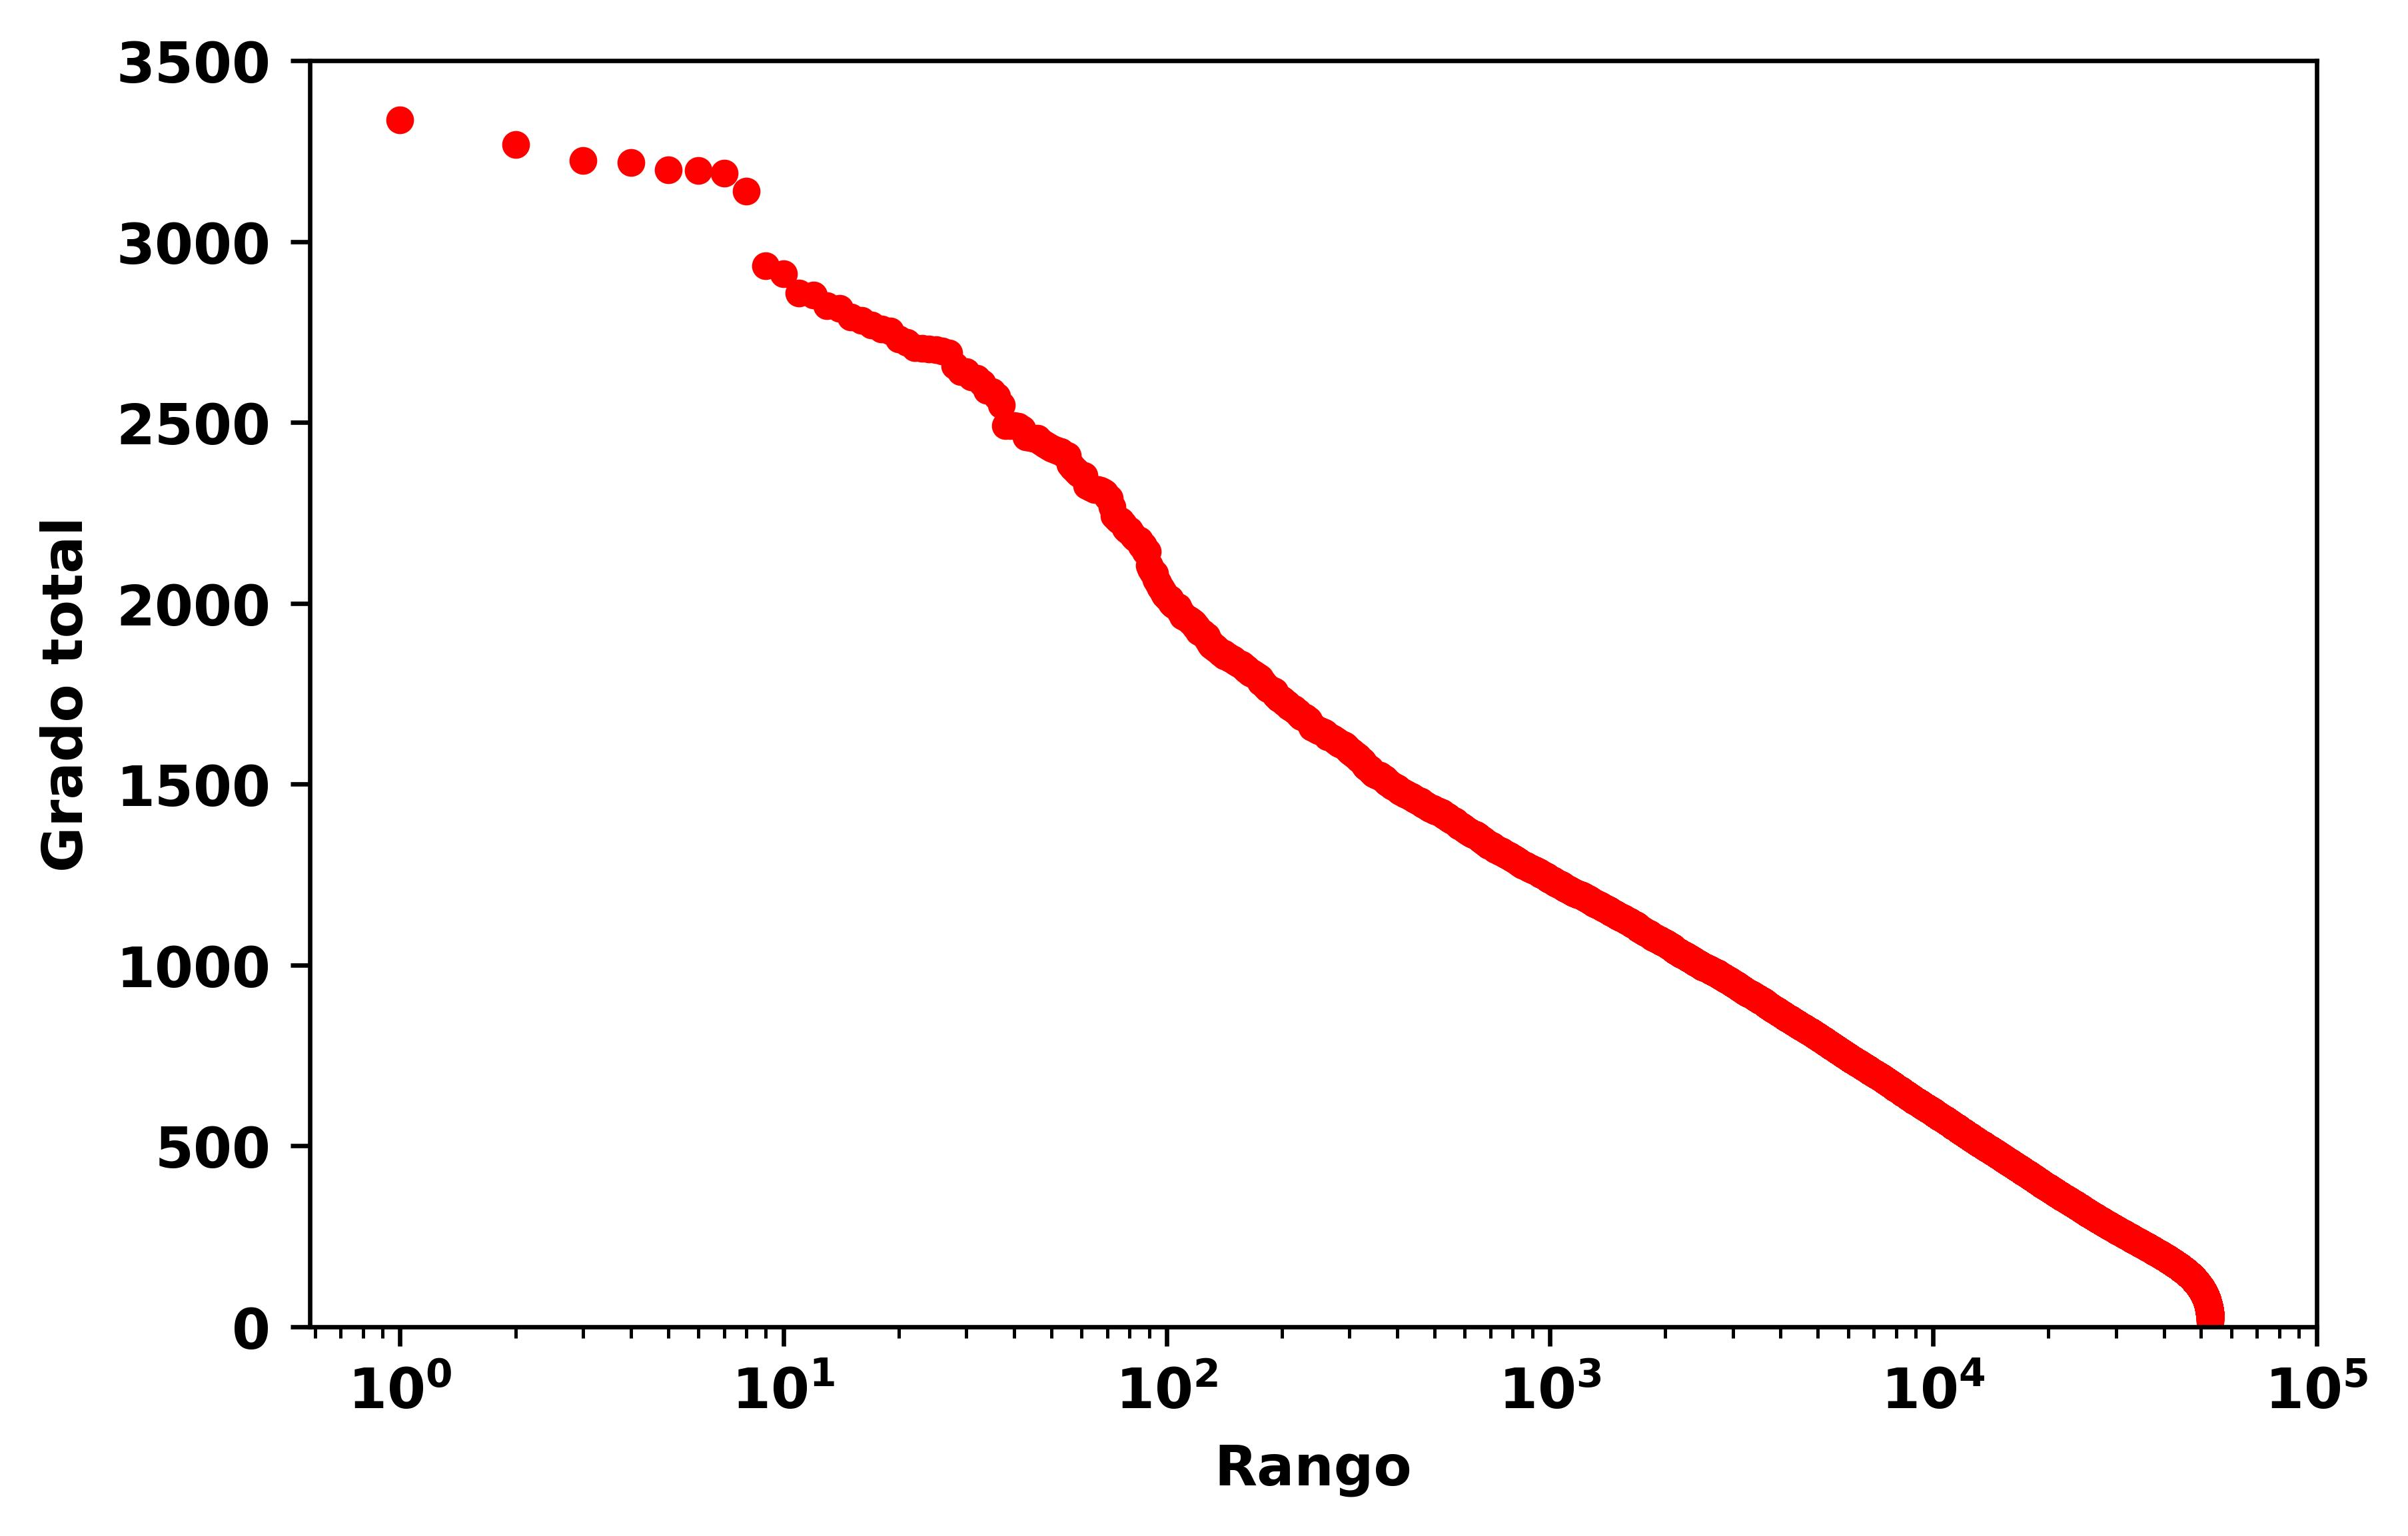
\includegraphics[width=\textwidth]{distributionLUAD.jpg}
	\caption{LUAD.}
	\label{fig:subfig11}
	\end{subfigure}
	\hfill
	
	\begin{subfigure}[b]{0.65\textwidth}
	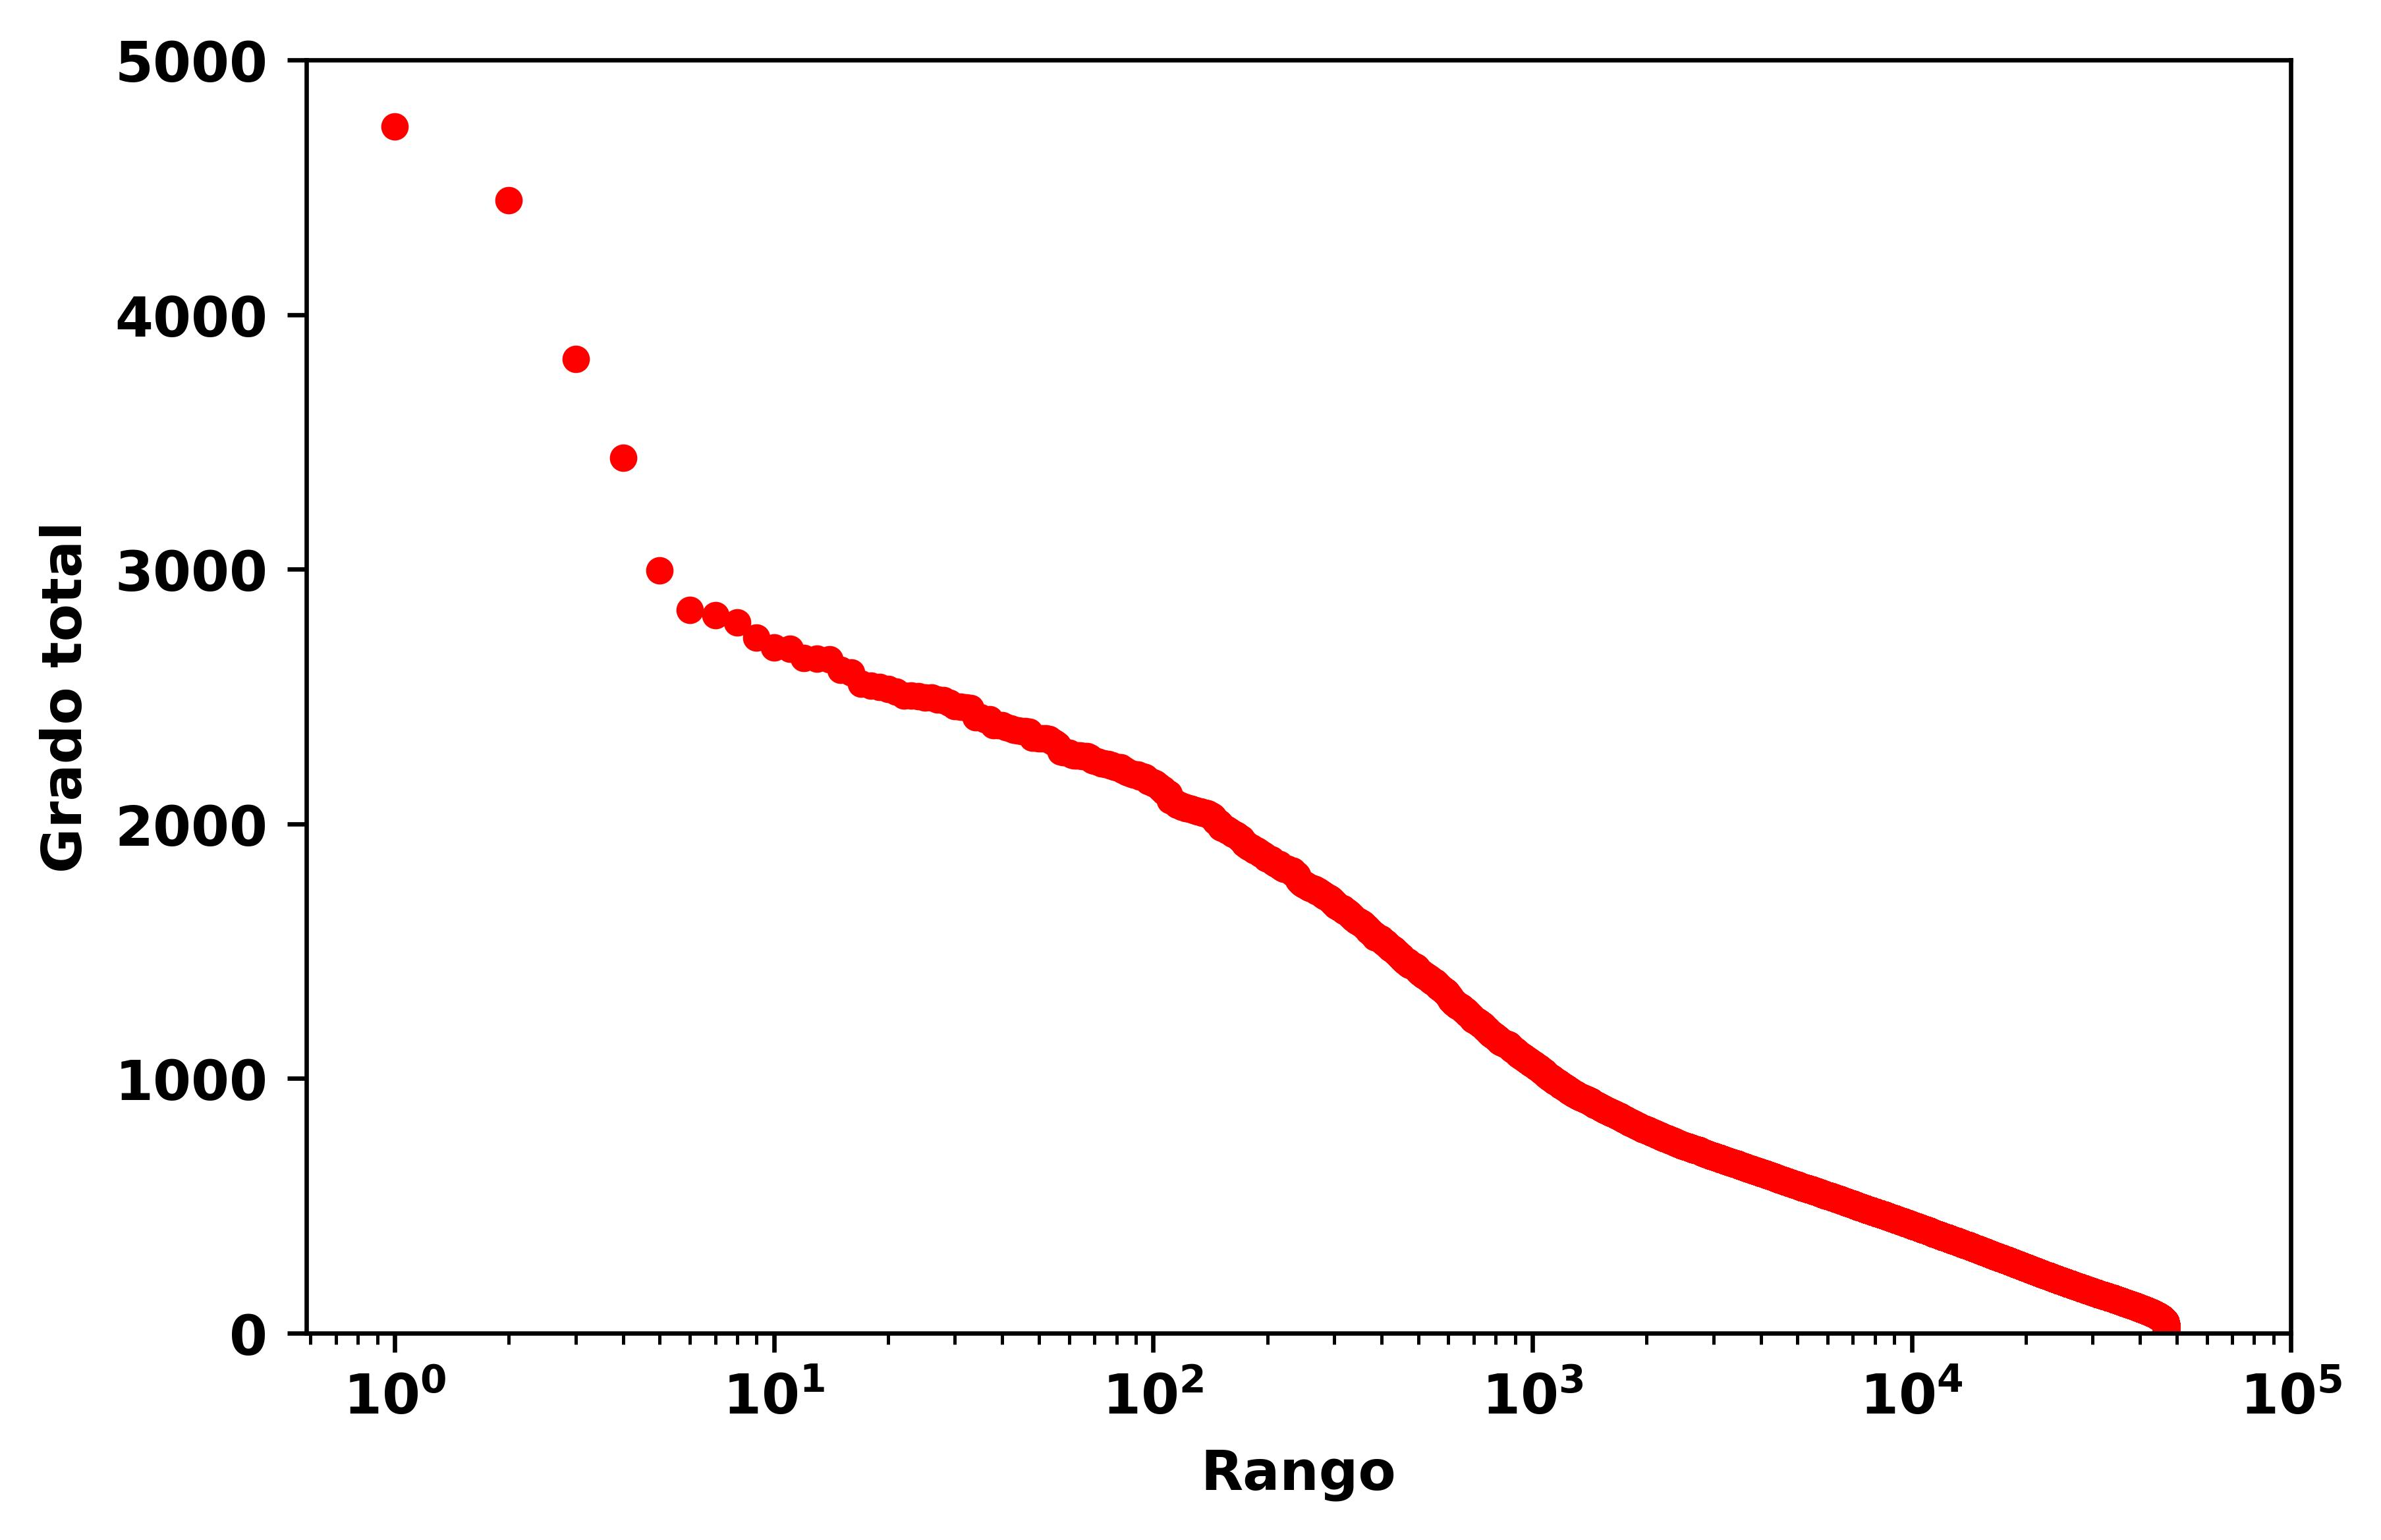
\includegraphics[width=\textwidth]{distributionPRAD.jpg}
	\caption{PRAD.}
	\label{fig:subfig21}
	\end{subfigure}
	\hfill
	
	\begin{subfigure}[b]{0.65\textwidth}
	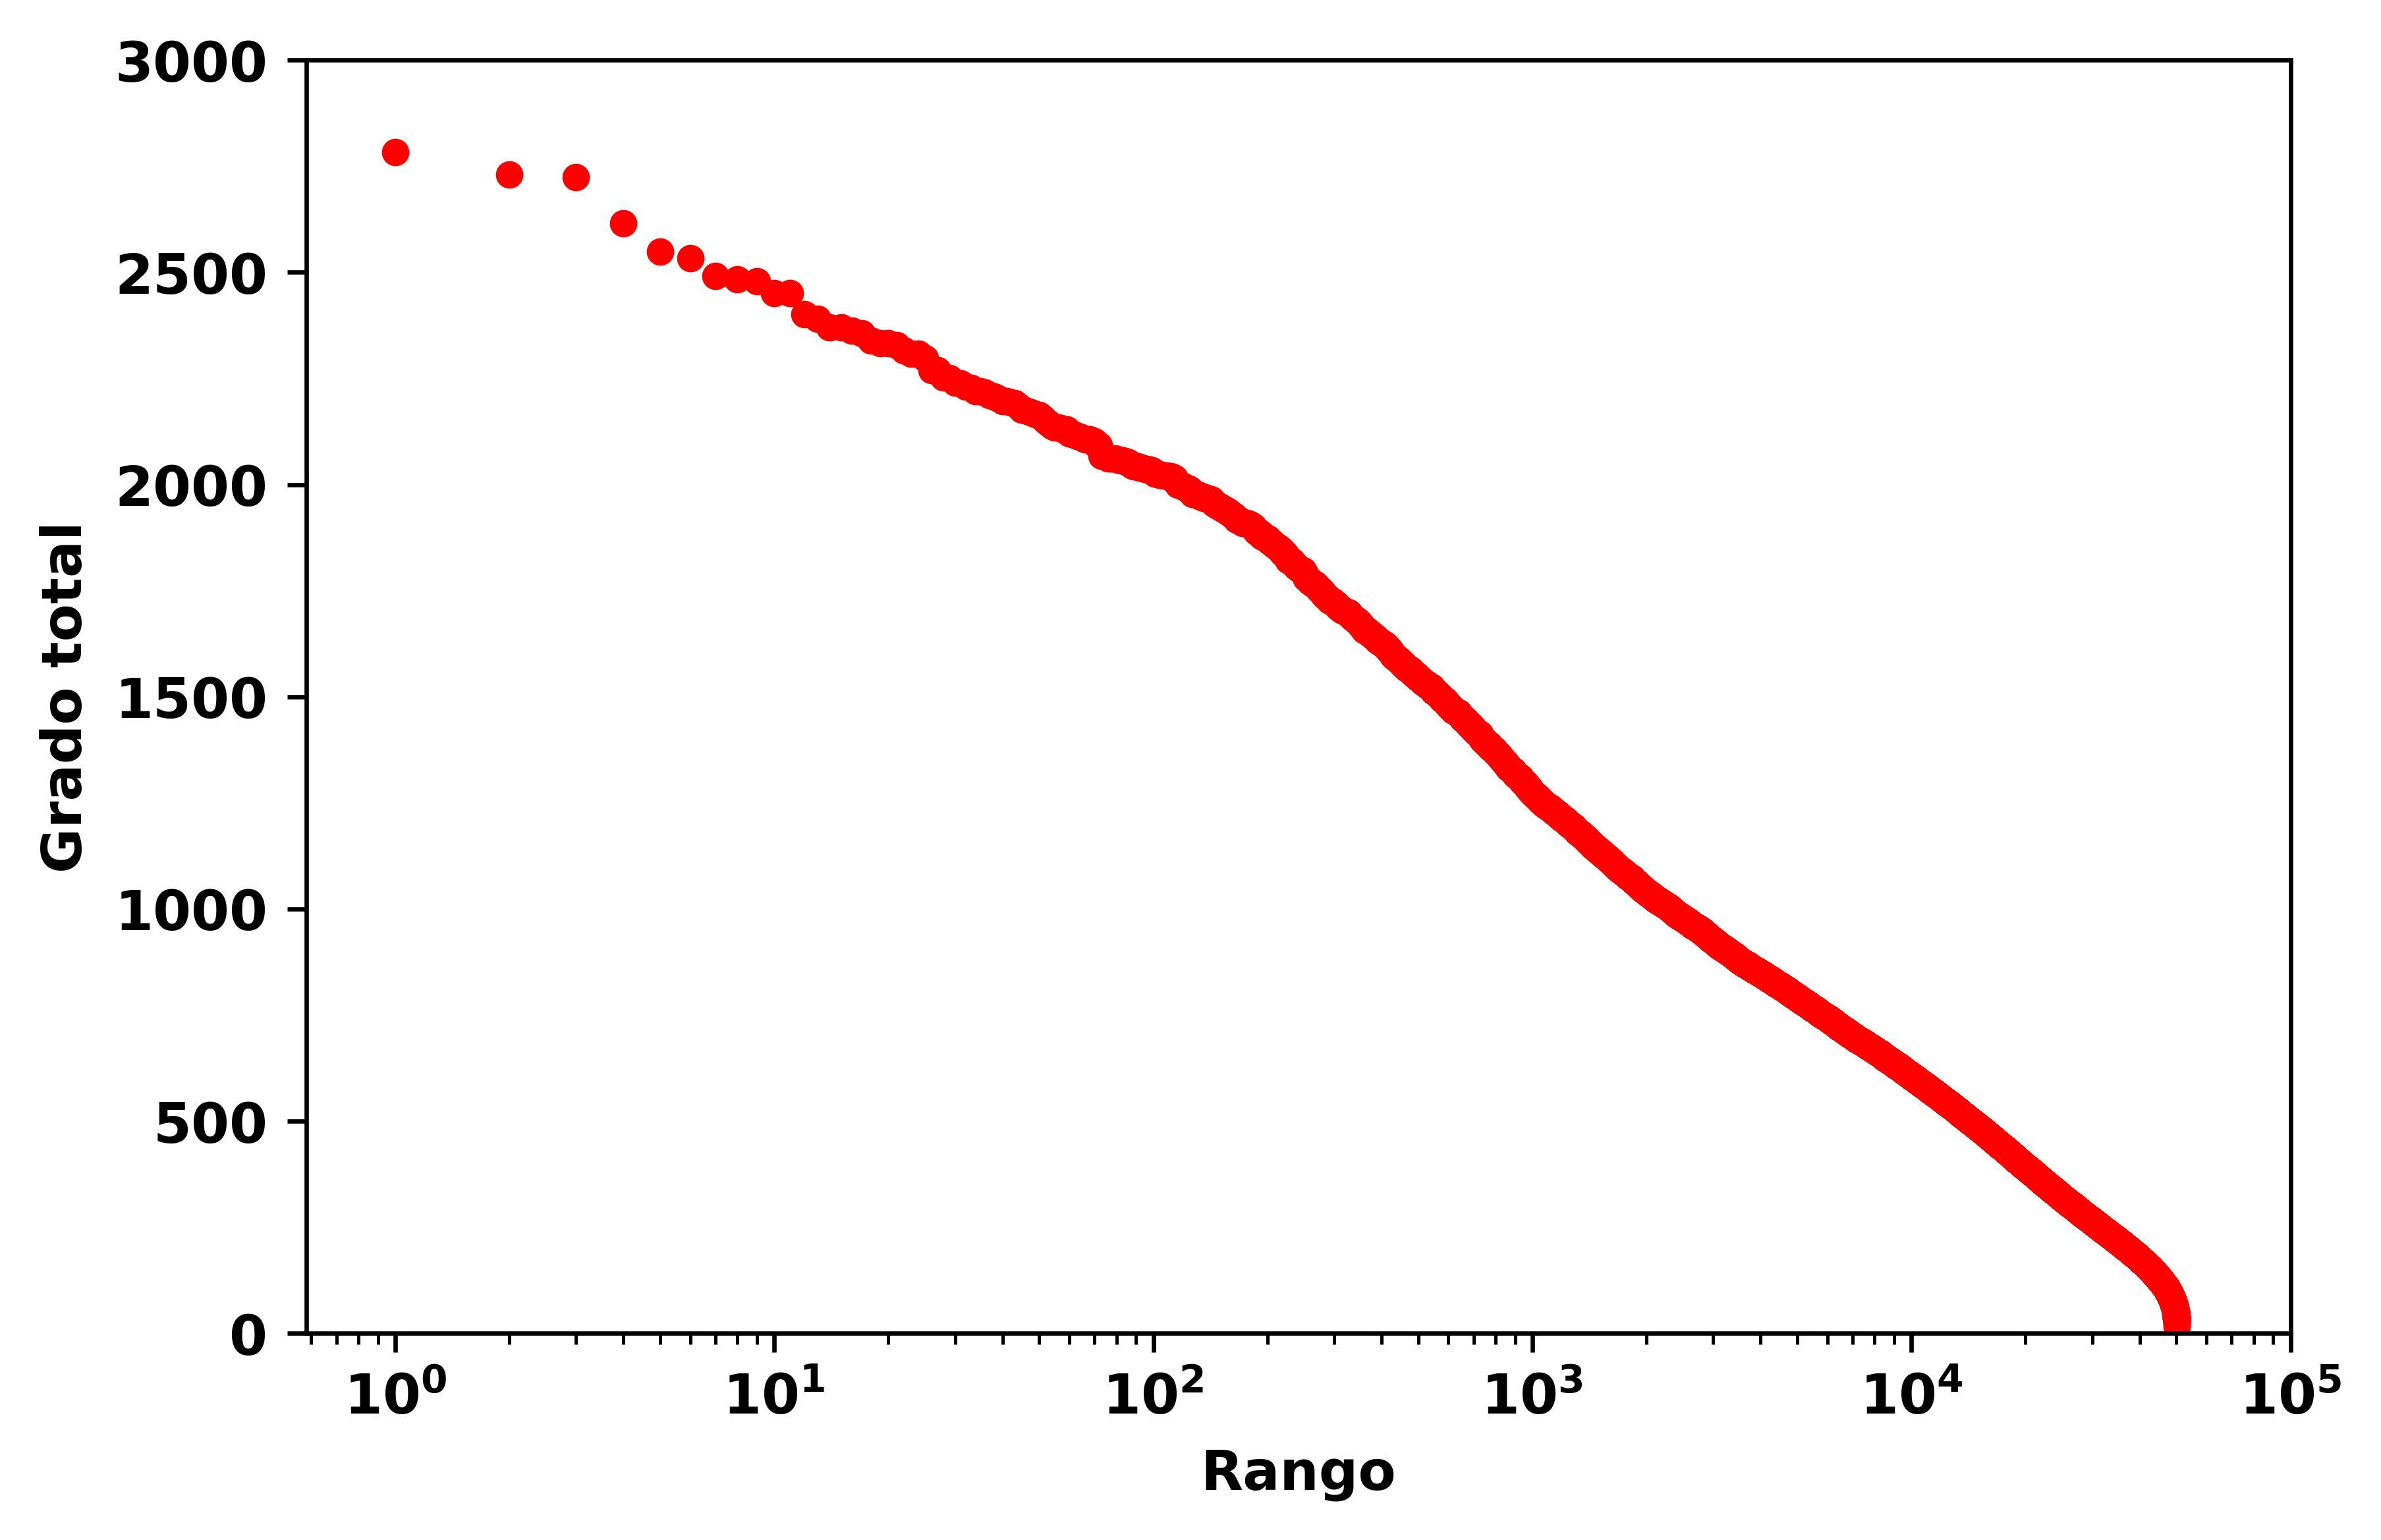
\includegraphics[width=\textwidth]{distributionLUSC.jpg}
	\caption{LUSC.}
	\label{fig:subfig31}
	\end{subfigure}
	\caption{Distribution of total degree as a function of vertex position in the ordered degree list, on a semi-logarithmic scale, for each network: (a) LUAD, (b) PRAD, (c) LUSC.}
	\label{fig:scale}
	
\end{figure}




\subsection{Analysis of relevant genes}
Once the gene deregulation causal networks had been constructed for the three tissues under study, their local topology was analyzed in order to identify genes that play a central role in the propagation of signals through the network. To this end, the centrality metrics mentioned in Section~\ref{sec:centralities} were calculated on the resulting graphs.
\\
For each network and each gene, all centrality metrics were computed and normalized by the maximum value recorded in the network. Thus, the values obtained for each metric lie between 0 and 1. Next, the total centrality of a gene was calculated as the sum of its four centralities, yielding values between 0 and 4. This procedure integrates different aspects of the structural prominence of a vertex in the network: its local connectivity, its role in causal routes, and its proximity to other vertices. Genes with the highest total centrality values are identified as candidate target genes, and the number of genes selected in this category depends on the distribution of total-centrality values in the corresponding tissue.
This methodology ensures that the selection of target genes is data-driven and reflects the hierarchical structure within each network.

Tables~\ref{tab:prad1}--~\ref{tab:lusc4} show the top 10 genes in the ranking of degree centrality, closeness, betweenness, and PageRank for PRAD, LUAD, and LUSC.

Figure~\ref{fig:centrali} shows the distribution of the 10 genes with the highest total centrality for each tissue. Based on this distribution, the genes shown in Table~\ref{tab:centralidades} were selected, accompanied by compact descriptions of the biological processes in which they are involved. To gather this additional information, the \textit{GeneCards} database was consulted\cite{GeneCards}.


\begin{table}[H]
\centering
\caption{Ranking of degree centrality of vertices corresponding to genes in PRAD.}
\label{tab:prad1}
\begin{tabular}{cccc}
\hline
\textbf{Position}         & \textbf{Vertex}     & \textbf{Gene}   & \textbf{Normalized centrality}   \\
\hline
   1       &     19846      &    MIR5682       &  1.000          \\
   2      &     232      &    PCGF7P       &     0.938       \\
   3       &     54      &    AC103810.5       &      0.807     \\
   4       &       954    &   DLX6        &       0.725    \\
   5       &       15721    &     RNA5SP361      &       0.631     \\
   6       &     1257      &   AL513523.2     &       0.599 \\
   7       &     17110      &   AC005410.1     &      0.594      \\
   8       &      42181     &   MTFR1        &      0.588      \\
   9       &      25479     &     KLHDC2      &       0.576 \\
   10       &     31700      &     AC092117.2      &       0.568     \\
\hline
\end{tabular}
\end{table}

\begin{table}[H]
\centering
\caption{Ranking of closeness centrality of vertices corresponding to genes in PRAD.}
\label{tab:prad2}
\begin{tabular}{cccc}
\hline
\textbf{Position}         & \textbf{Vertex}     & \textbf{Gene}   & \textbf{Normalized centrality}   \\
\hline
   1       &     19846      &    MIR5682       &   1.000         \\
   2      &      19126     &     Y\_RNA      &       0.845     \\
   3       &      1172     &      AL513523.2     &         0.833   \\
   4       &      44677     &   AC097460.2        &  0.825          \\
   5       &      46922     &    (ENSG00000280861)       &         0.761   \\
   6       &     24179      &     WDR13      &  0.737          \\
   7       &     40590      &      AL109947.1     &     0.737       \\
   8       &     46096      &    KRT17P7       &  0.684          \\
   9       &      4241     &      HLA-L     &       0.683     \\
   10       &       866    &       VTA1    &       0.675     \\
\hline
\end{tabular}
\end{table}

\begin{table}[H]
\centering
\caption{Ranking of betweenness centrality of vertices corresponding to genes in PRAD.}
\label{tab:prad3}
\begin{tabular}{cccc}
\hline
\textbf{Position}         & \textbf{Vertex}     & \textbf{Gene}   & \textbf{Normalized centrality}   \\
\hline
   1       &    7382       &     AC138028.3      &   1.000 \\
   2      &      23466     &       (ENSG00000281891)    &0.778            \\
   3       &      26231     &     LINC00847      & 0.762           \\
   4       &     45457      &    BPIFB4       &    0.676        \\
   5       &     18728      &      AL359551.1     &  0.641          \\
   6       &     4213      &     Y\_RNA      &   0.625         \\
   7       &     38729      &     HMGB1P13      &    0.599        \\
   8       &     44072      &   PTGDR        &    0.590 \\
   9       &      11734     &    AC068790.7       &      0.561      \\
   10       &       1866    &    TREML1       &    0.536        \\
\hline
\end{tabular}
\end{table}

\begin{table}[H]
\centering
\caption{Ranking of PageRank of vertices corresponding to genes in PRAD.}
\label{tab:prad4}
\begin{tabular}{cccc}
\hline
\textbf{Position}         & \textbf{Vertex}     & \textbf{Gene}   & \textbf{Normalized centrality}   \\
\hline
   1    & 19846  &   MIR5682                &  1.000          \\
   2    & 19126 &      Y\_RNA            &      0.294      \\
   3    & 1172  &     AL513523.2                &      0.228      \\
   4    & 44677  &   AC097460.2                  &    0.136        \\
   5    & 46922  &   (ENSG00000280861)                  &     0.118       \\
   6    & 40590  &     AL109947.1             &  0.099          \\
   7   &  24179  &     WDR13              &      0.086      \\
   8   &  4241  &     HLA-L                 &     0.572       \\
   9   &  11605  &      NOTCH2NLA                &   0.504         \\
   10   &  20668  &     RPL37P2                &      0.041      \\
\hline
\end{tabular}
\end{table}



\begin{table}[H]
\centering
\caption{Ranking of degree centrality of vertices corresponding to genes in LUAD.}
\label{tab:luad1}
\begin{tabular}{cccc}
\hline
\textbf{Position}         & \textbf{Vertex}     & \textbf{Gene}   & \textbf{Normalized centrality}   \\
\hline
   1       &    20442       &  SNORA74C-1         &           1.000 \\
   2      &     15107      & SRSF8CP        &    0.979        \\
   3       &    41561       & AC090164.2          &           0.966 \\
   4       &    11475       &  BNIP3P37         &0.964            \\
   5       &    16844       & RNU6-948P          &  0.958          \\
   6       &    49413       &   MIR6504        & 0.958           \\
   7       &    6021       &    FAM3B       &  0.956          \\
   8       &    12232       &    NEURL1B       & 0.941           \\
   9       &    38433       &    PIP4K2B       &    0.879        \\
   10       &   26273        &      IGLV11-55     &           0.872 \\
\hline
\end{tabular}
\end{table}

\begin{table}[H]
\centering
\caption{Ranking of closeness centrality of vertices corresponding to genes in LUAD.}
\label{tab:luad2}
\begin{tabular}{cccc}
\hline
\textbf{Position}         & \textbf{Vertex}     & \textbf{Gene}   & \textbf{Normalized centrality}   \\
\hline
   1       &    4414       &  AC079035.1         &  1.000          \\
   2      & 34427          &  FAM153A         &   0.991         \\
   3       &     45859      &  AC134349.2         &   0.989         \\
   4       &24997           &   DNAJC7        &   0.988         \\
   5       &     36569      &     KIR3DL3      &   0.986         \\
   6       &  41982         &   ABCB11        &   0.986         \\
   7       &   40570        &     AC004130.2      &   0.984         \\
   8       &    42854       &    (ENSG00000276283)       &   0.981         \\
   9       &     2378      &   LINC01163        &   0.980         \\
   10       &        38008   &  SLC545         &   0.979         \\
\hline
\end{tabular}
\end{table}

\begin{table}[H]
\centering
\caption{Ranking of betweenness centrality of vertices corresponding to genes in LUAD.}
\label{tab:luad3}
\begin{tabular}{cccc}
\hline
\textbf{Position}         & \textbf{Vertex}     & \textbf{Gene}   & \textbf{Normalized centrality}   \\
\hline
   1       &    31646       &   LINC02605        &  1.000          \\
   2      &     44909      &    (ENSG00000275707)       &   0.813         \\
   3       &     49080      &     WDR82P2      &   0.772         \\
   4       &    33552       &   AL592546.2        &   0.564         \\
   5       &     32857      &    DNAL4       &   0.490         \\
   6       &     12741      &    IGHV1-2       &   0.477         \\
   7       &     3815      &     EML4      &    0.471        \\
   8       &     9097      &     CYP2U1      &   0.461         \\
   9       &     18816      &     C7orf65      &     0.454       \\
   10       &    37657       &     AC008982.2      &  0.422          \\
\hline
\end{tabular}
\end{table}

\begin{table}[H]
\centering
\caption{Ranking of PageRank of vertices corresponding to genes in LUAD.}
\label{tab:luad4}
\begin{tabular}{cccc}
\hline
\textbf{Position}         & \textbf{Vertex}     & \textbf{Gene}   & \textbf{Normalized centrality}   \\
\hline
   1       &    45859       &    AC134349.2       &  1.000          \\
   2      &   34427        & FAM153A          &0.867            \\
   3       &   37844        & AC239809.3          & 0.612           \\
   4       &    15107       &   SRSF8CP        &    0.494        \\
   5       &     50606      &    RN7SL379P       &   0.398         \\
   6       &    30866       &  AC009060.1         & 0.379           \\
   7       &  6206         &  AC073418.1         & 0.328           \\
   8       &   6873        &    SLC6A5       &   0.308         \\
   9       &    40570       &     AC004130.2      &           0.302 \\
   10       &    29121       &    PPP1R27       &  0.295          \\
\hline
\end{tabular}
\end{table}



\begin{table}[H]
\centering
\caption{Ranking of degree centrality of vertices corresponding to genes in LUSC.}
\label{tab:lusc1}
\begin{tabular}{cccc}
\hline
\textbf{Position}         & \textbf{Vertex}     & \textbf{Gene}   & \textbf{Normalized centrality}   \\
\hline
   1       &    30177       &   MPRiP        & 1.000           \\
   2      &   9391        &  AC110995.1         &  0.980          \\
   3       &   24485        &  LINC02320         & 0.978           \\
   4       &    46861       & MIR6504          & 0.939           \\
   5       &   7490        &    KANSL1-AS1       &     0.915       \\
   6       &       26466    &  KDM2A         & 0.910           \\
   7       &      8219     &      DACH1-IT2     &     0.895       \\
   8       &      35643     &     CREB3      & 0.892           \\
   9       &      43961     &     (ENSG00000274182)      &   0.890         \\
   10       &    21102       &      RNU6-1187P     &   0.880         \\
\hline
\end{tabular}
\end{table}

\begin{table}[H]
\centering
\caption{Ranking of closeness centrality of vertices corresponding to genes in LUSC.}
\label{tab:lusc2}
\begin{tabular}{cccc}
\hline
\textbf{Position}         & \textbf{Vertex}     & \textbf{Gene}   & \textbf{Normalized centrality}   \\
\hline
   1       &    36822       &   SIRLNT        &   1.000         \\
   2      &     18174      &    AL356585.4       &   0.940         \\
   3       &     5970      &  AC010501.1         &   0.939         \\
   4       &     1989      &   ARMH1        &      0.938      \\
   5       &     47367      &    TPD52       &  0.937          \\
   6       &     22987      &    HMGB3P8       &     0.937       \\
   7       &     45167      &    RTL8C       &      0.936      \\
   8       &     23296      &    AC009531.1       &      0.935      \\
   9       &      49807     &   ERVK9-11        & 0.935           \\
   10       &      22960     &     C0G7      &      0.935      \\
\hline
\end{tabular}
\end{table}

\begin{table}[H]
\centering
\caption{Ranking of betweenness centrality of vertices corresponding to genes in LUSC.}
\label{tab:lusc3}
\begin{tabular}{cccc}
\hline
\textbf{Position}         & \textbf{Vertex}     & \textbf{Gene}   & \textbf{Normalized centrality}   \\
\hline
   1    &36527   &     CSAD            &    1.000        \\
   2      &39964&      DEAF1               &    0.910        \\
   3      &14911  &     AC020910.5                 &           0.797 \\
   4      &4471 &    AC017067.1                  &           0.744 \\
   5  &42133     &    FKBP3                  &0.710            \\
   6      & 22598 &    ACVRL1                  & 0.706           \\
   7       & 46314 &    CD46                  & 0.687           \\
   8       & 35729&     U6                & 0.682           \\
   9       & 22793 &    ERAL1               & 0.644           \\
   10       & 3953 &    (ENSG00000273581)                &           0.634 \\
\hline
\end{tabular}
\end{table}

\begin{table}[H]
\centering
\caption{Ranking of PageRank of vertices corresponding to genes in LUSC.}
\label{tab:lusc4}
\begin{tabular}{cccc}
\hline
\textbf{Position}         & \textbf{Vertex}     & \textbf{Gene}   & \textbf{Normalized centrality}   \\
\hline
   1       &   36822        &   SIRLNT        &  1.000          \\
   2      &     32280      &     OR1X5P      &     0.110       \\
   3       &    24834       &    CYSLTR1       &    0.079        \\
   4       &    4530       &     EEF1AKMT1      &    0.048        \\
   5       &    1989       &   ARMH1        &    0.038        \\
   6       &    12720       &    PINLYP       &    0.037        \\
   7       &    907       &        NIF3L1   &      0.034      \\
   8       &    6959       &      AL136307.1     &   0.032         \\
   9       &     16902      &  WDR82P1         &      0.032      \\
   10       &     22987      &  HMGB3P8         &      0.028      \\
\hline
\end{tabular}
\end{table}


\begin{figure}[H]
	\centering
	\begin{subfigure}[b]{0.65\textwidth}
	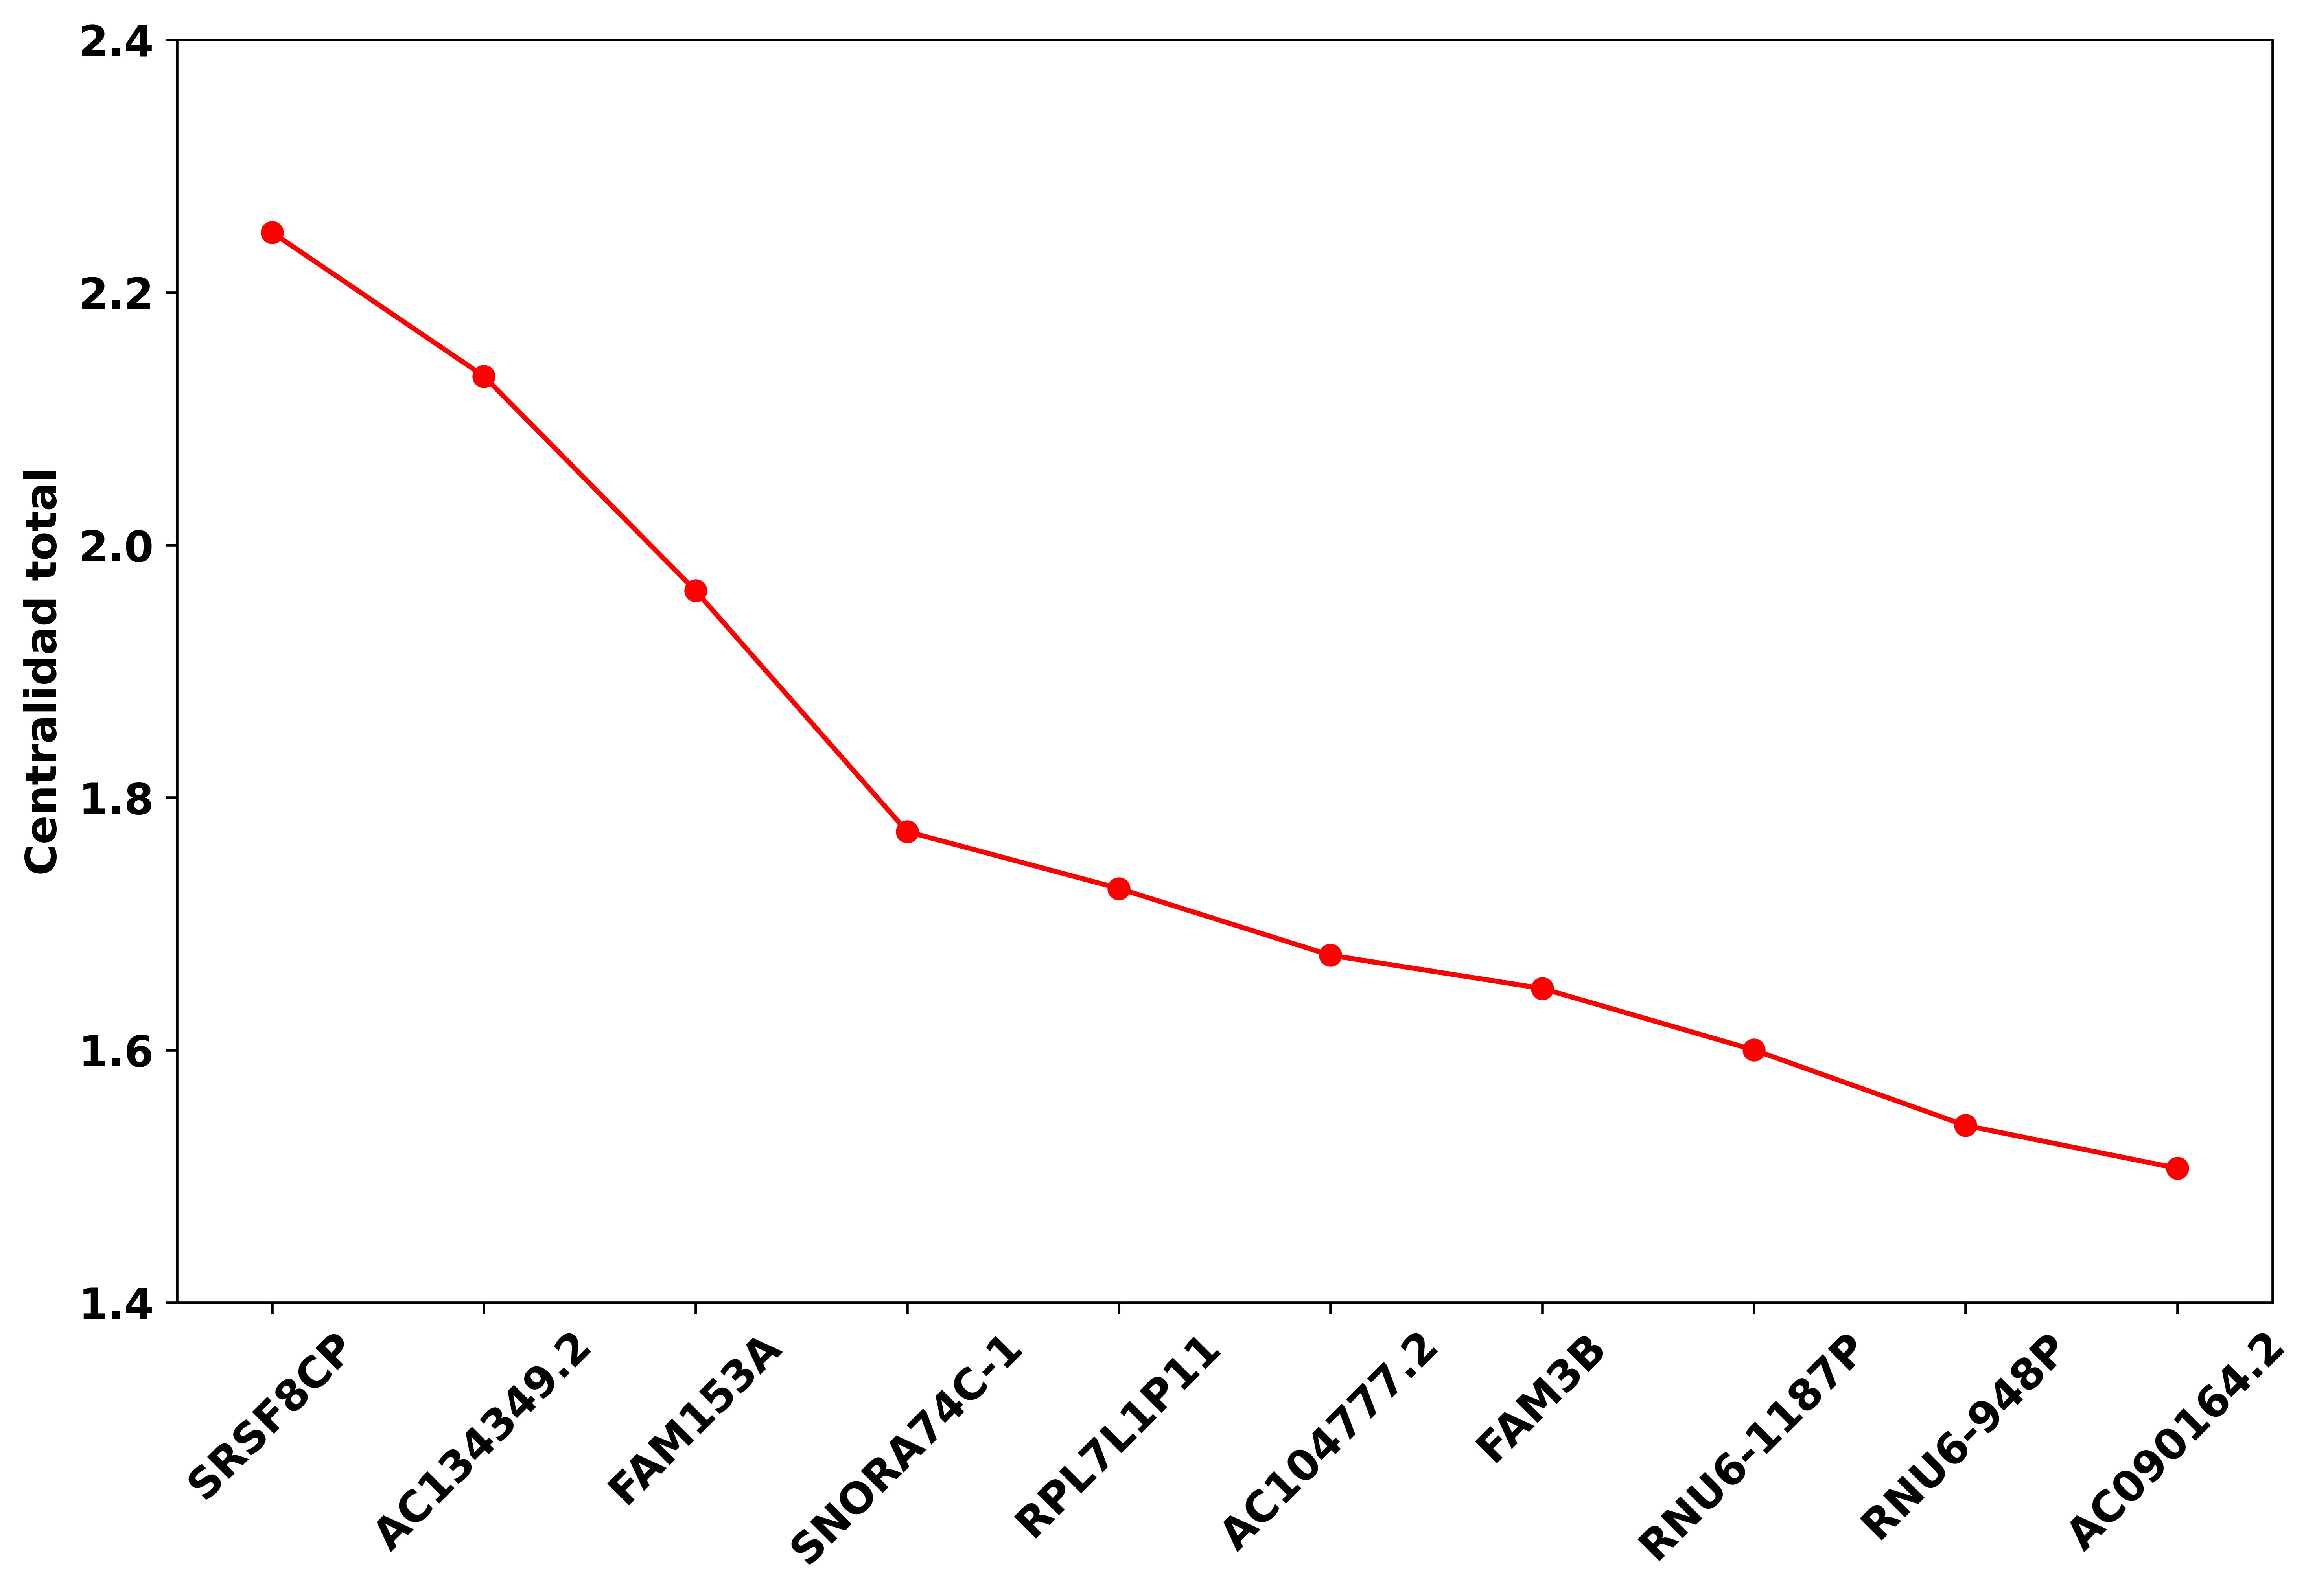
\includegraphics[width=\textwidth]{LUAD.jpg}
	\caption{LUAD.}
	\label{fig:subfig1}
	\end{subfigure}
	\hfill
	
	\begin{subfigure}[b]{0.65\textwidth}
	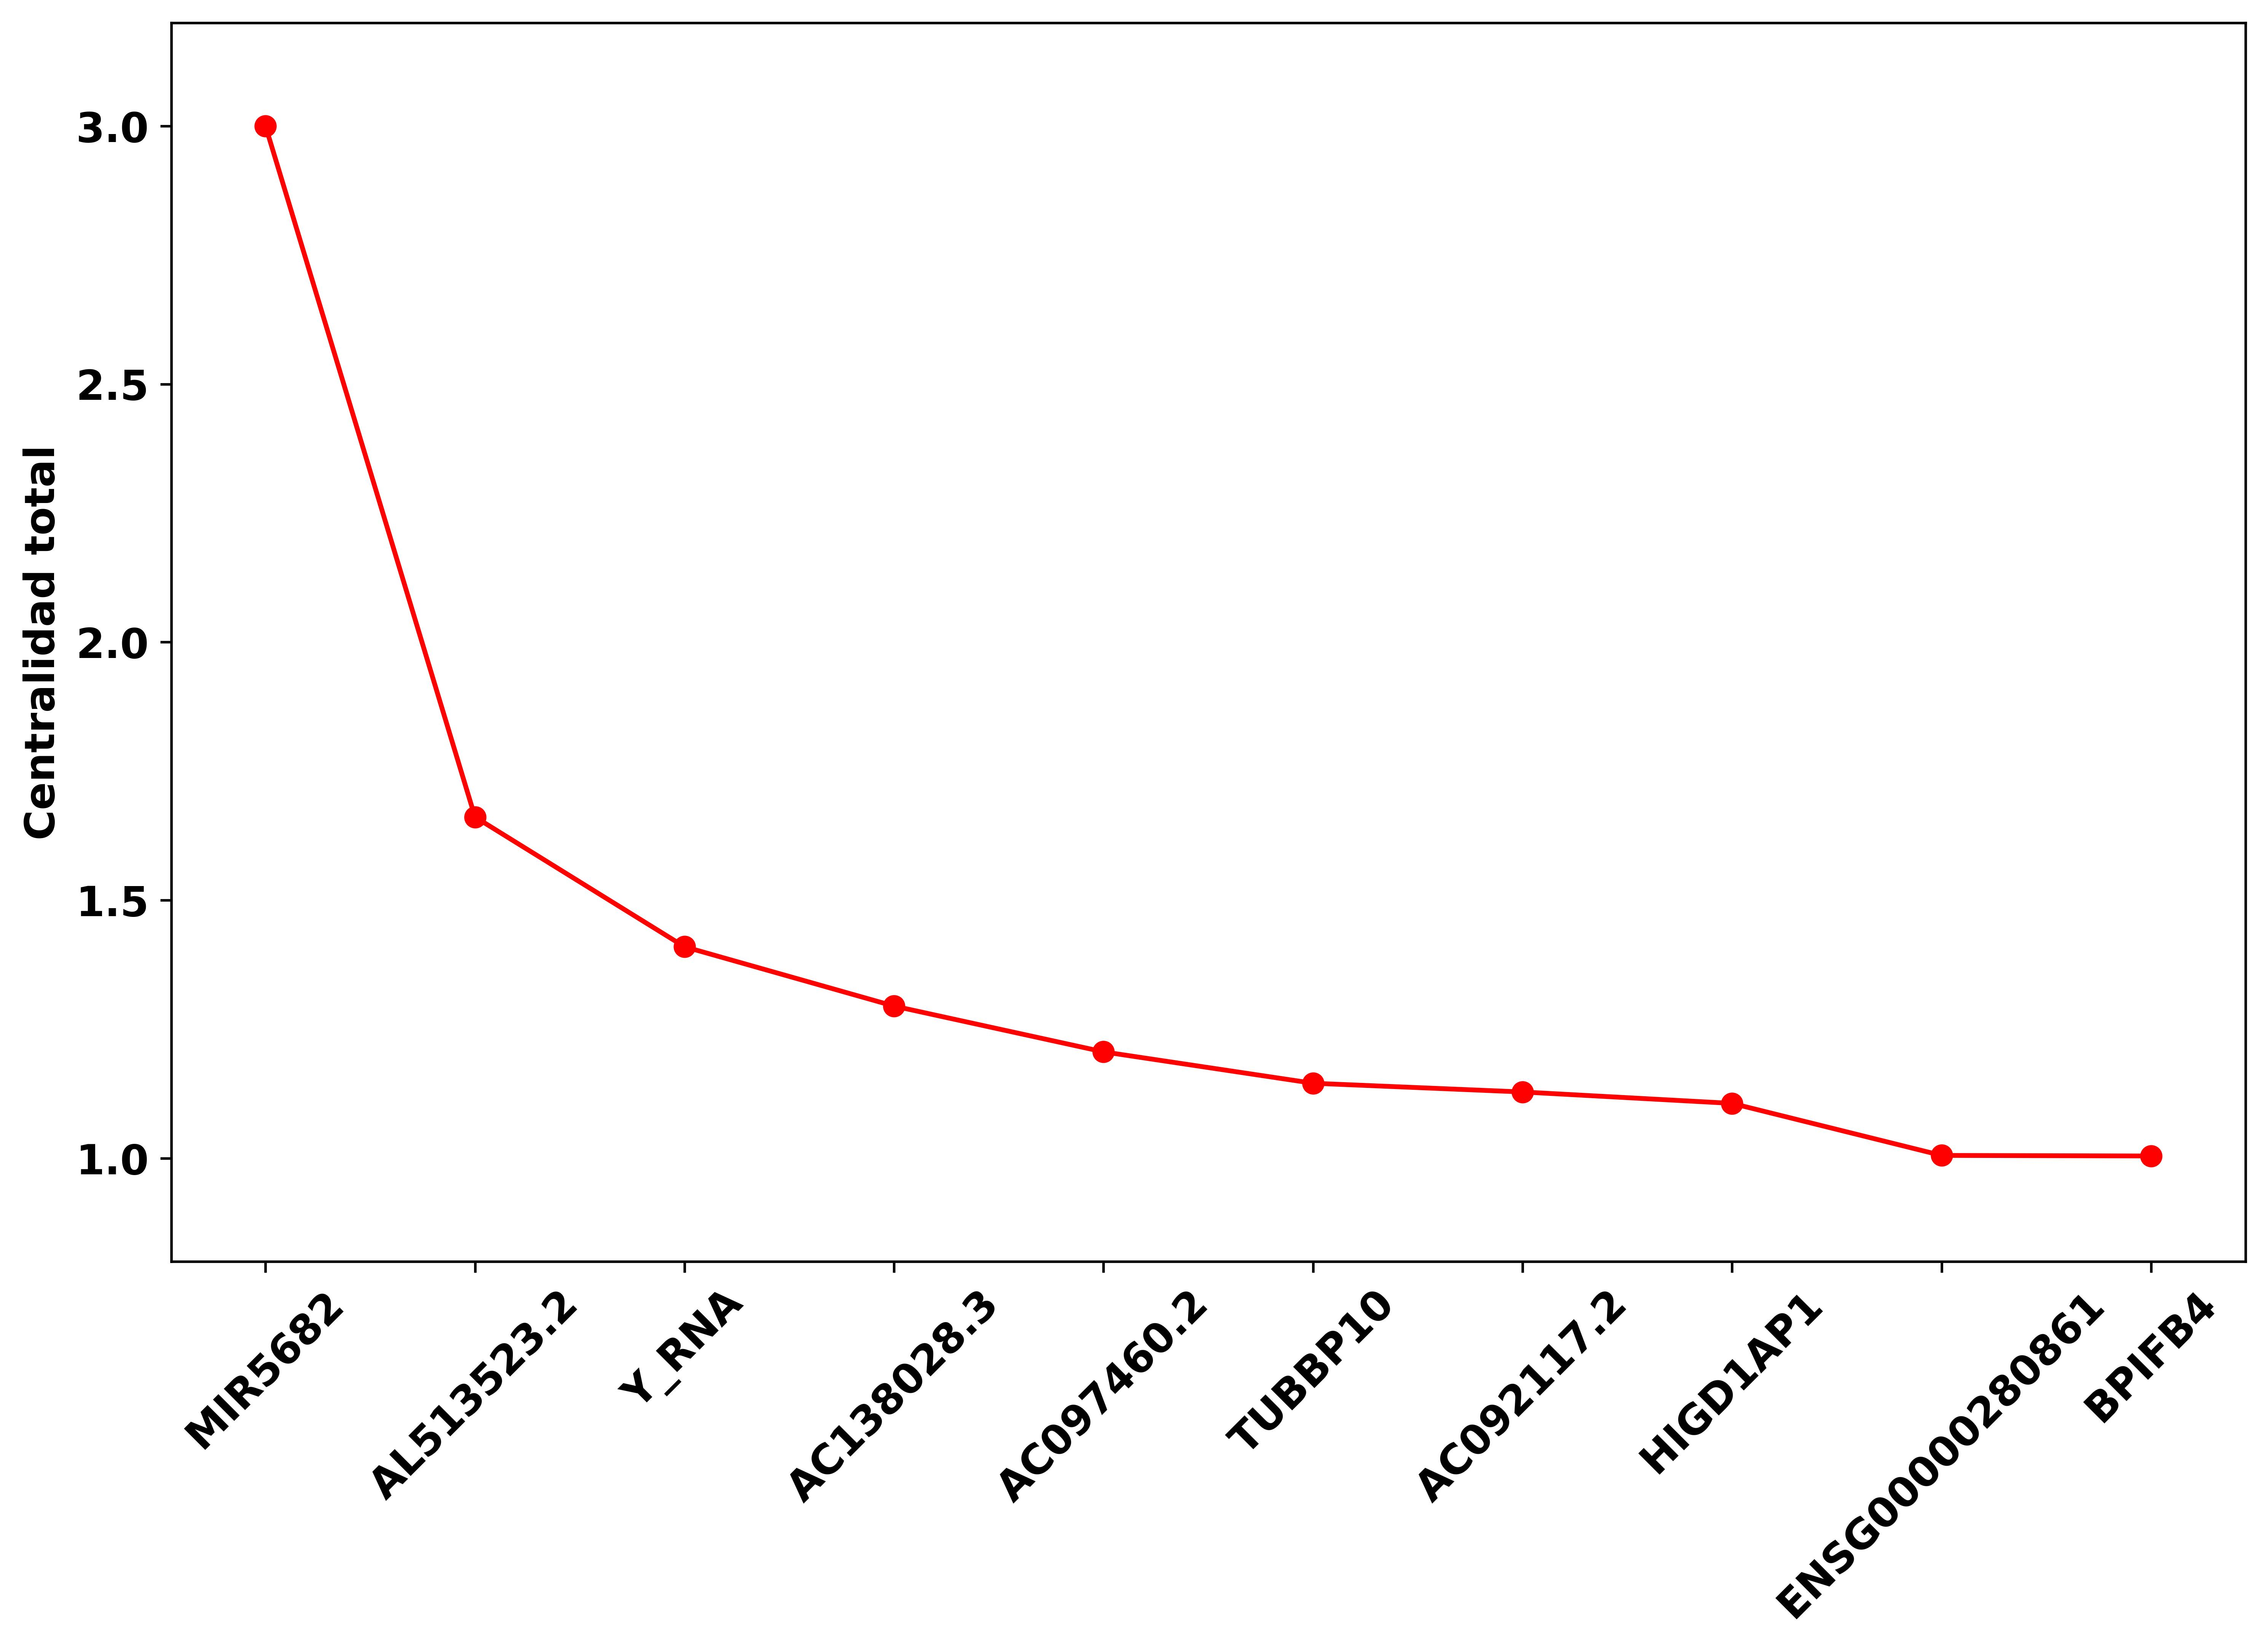
\includegraphics[width=\textwidth]{PRAD.jpg}
	\caption{PRAD.}
	\label{fig:subfig2}
	\end{subfigure}
	\hfill
	
	\begin{subfigure}[b]{0.65\textwidth}
	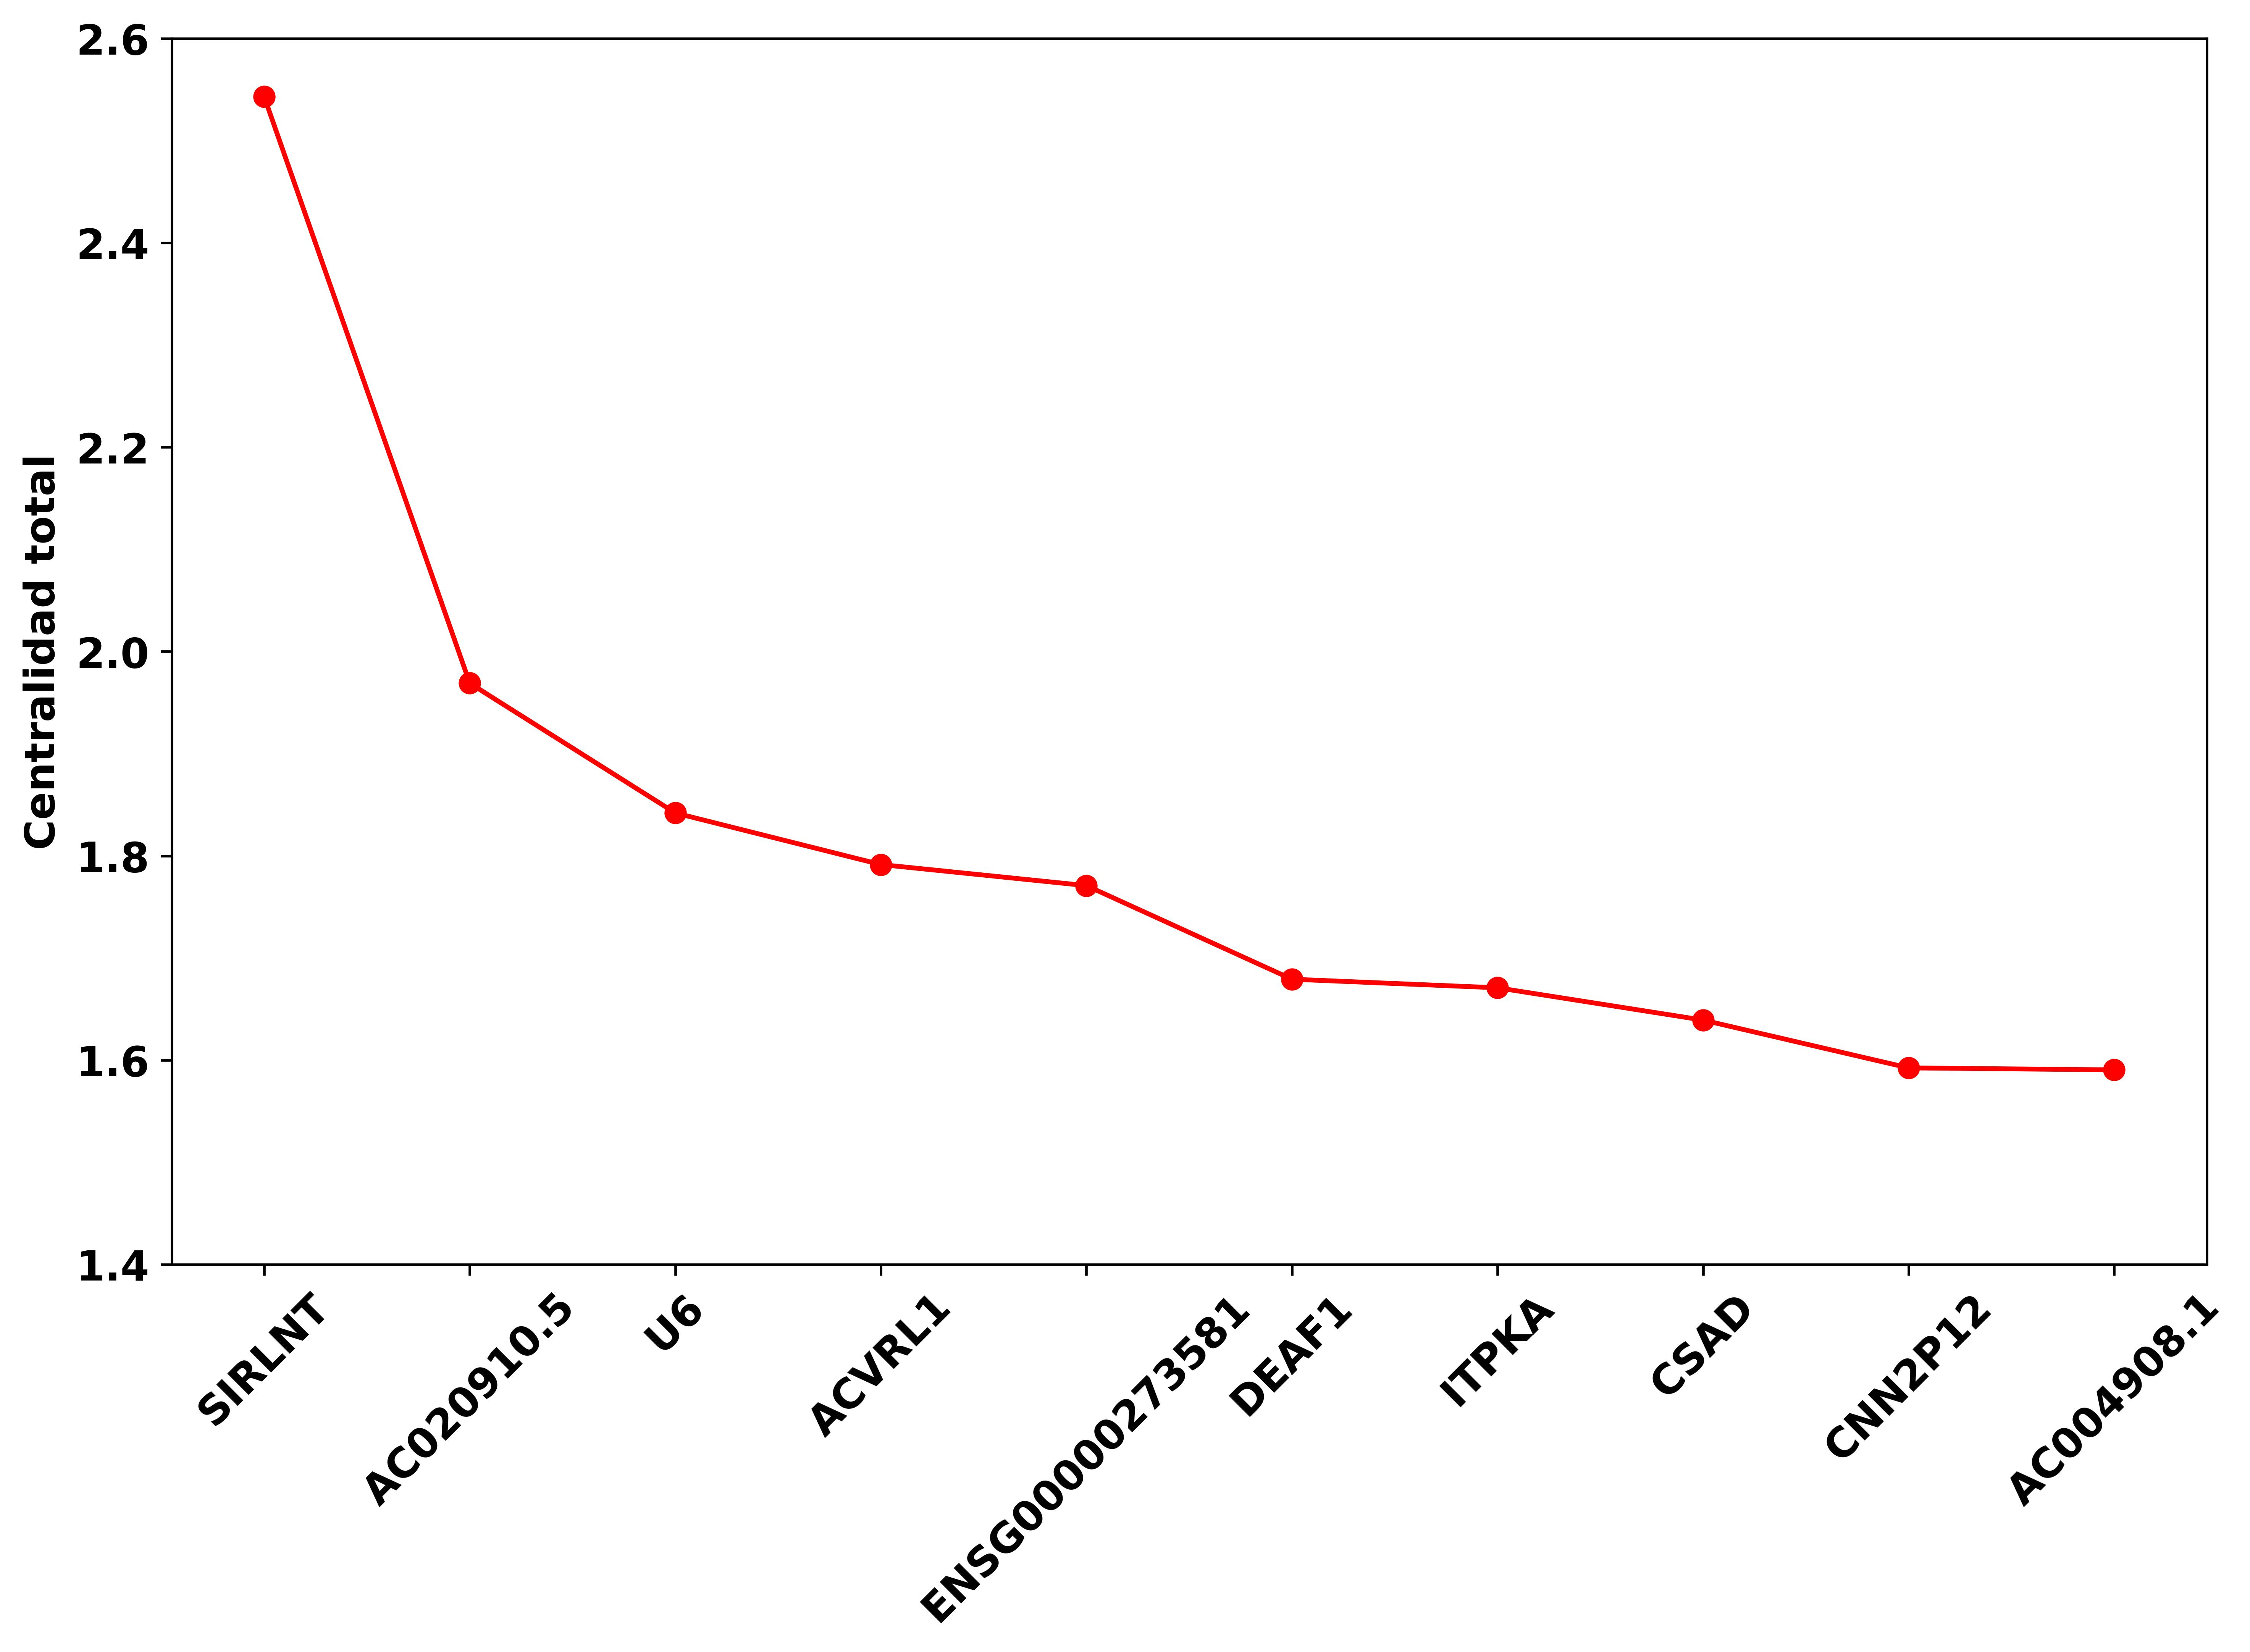
\includegraphics[width=\textwidth]{LUSC.jpg}
	\caption{LUSC.}
	\label{fig:subfig3}
	\end{subfigure}
	\caption{Distribution of total centralities for each tissue: (a) LUAD, (b) PRAD, (c) LUSC.}
	\label{fig:centrali}
	
\end{figure}

\begin{table}[H]
\centering
\caption{Selected target genes and their description in the corresponding tissue.}
\label{tab:centralidades}
\begin{tabular}{llll}
\hline
\textbf{Tissue} & \textbf{Gene}        & \textbf{Full name}          & \textbf{Description}                \\
\hline
PRAD            & MIR5682             & MicroRNA 5682            & Overexpressed in metastatic \\
 & &  & prostate cancer; associated with \\
 & & & tumor progression\cite{metastasis} \\
 &&&\\
\hline
LUAD            & SRSF8CP            & Pseudogene of serine/arginine-rich   & Information not available                     \\
 & & splicing factor & \\
 & & 8C & \\
&&&\\
\hline
LUSC            & SIRLNT          & SIRT1 tumor-promoting   & Information not available                     \\
 & & regulator lncRNA  & \\
 & &  & \\
&&&\\
\hline
\end{tabular}
\end{table}



It should be noted that the gene \textit{MIR5682}, identified as a relevant target in the PRAD gene deregulation network, has been reported in the literature as significantly overexpressed in metastatic prostate cancer, suggesting a possible functional role in tumor progression processes\cite{metastasis}. Its prominent presence in the inferred causal network reinforces the hypothesis of its involvement in key mechanisms of gene regulation associated with prostate carcinogenesis.

\newpage

% ====================
% Conclusions and Recommendations
% ====================
\chapter*{Conclusions}

In this work, a new nonparametric causal discovery method, implemented in the \texttt{CChains} code and aimed at inferring gene deregulation networks from binary gene expression data, was validated. The proposed validation relies on graph-theory tools to represent and analyze the inferred networks.

In a first stage, the method was quantitatively validated using synthetic data generated from known causal graphs. Under reasonable assumptions about the underlying causal model and the distribution of the exogenous variables on which it depends, a simulation methodology was designed to evaluate the algorithm performance in controlled scenarios.

Subsequently, the method was applied to real gene expression data obtained from the TCGA repository, corresponding to three tissue types: prostate adenocarcinoma, lung adenocarcinoma, and lung squamous cell carcinoma. In each case, a gene deregulation causal network was constructed from normal and tumor samples, and its topological properties were analyzed using both global and local graph-theory metrics.

Once the networks were obtained, centrality metrics (degree, betweenness, closeness, and PageRank) were applied to identify vertices of structural importance, which can be interpreted as genes potentially relevant to the regulation of the carcinogenic process. This information provides a complementary route for generating biological hypotheses, identifying candidate therapeutic target genes, and studying the functional architecture of the deregulation network.

\chapter*{Recommendations}

\begin{itemize}
\item Extend validation to DAGs with more complex structures and to graphs with dimensions and local metrics comparable to those obtained from real data.

\item Explore the performance of the causal discovery method in the case of causal models with immoralities described by structural equations with logical conjunctions between endogenous variables. The causal discovery algorithm was designed to study causal quasi-sufficiency relationships. However, it is not known how the inference of these relationships could be affected when more complex causal relationships exist in the underlying network, where endogenous contributory causes may be present.

\item Carry out an exhaustive and detailed analysis of cases in which real edges are eliminated in graphs with immoralities and DAGs.

\item Implement optimizations and parallelize the phases of the algorithm whenever possible. Since this is genuine \textit{big data}, with more than 60,000 genes and between hundreds and thousands of samples, the computational performance of the causal discovery algorithm must be improved.

\item Explore a protocol for selecting the Loevinger threshold (\(H_0\)), the only parameter of the causal discovery method. So far, a value motivated by probabilistic-causality arguments has been used. However, this value may not be optimal for discovering the largest possible number of causal relationships from observational data. On the other hand, different data sets may require a different \(H_0\) value to obtain the same performance in terms of recovery of real causal relationships. The design of automatic adjustment schemes for this single free parameter is suggested, for example through the principle of minimal sensitivity (PMS) or greedy search.

\item Study the influence of preprocessing on causal inference by analyzing how different binarization schemes (alternative thresholds, normalization methods) affect the inferred topology.

\item Perform an analysis of the temporal and spatial complexity of the \texttt{CChains} method in comparison with algorithms based on conditional independence, such as PC. This would make it possible to quantify the scalability and practical limits of each approach as a function of the number of genes and samples.

\item Incorporate additional centrality metrics such as \emph{eigenvector} centrality and weighted betweenness centrality to identify regulatory genes. Likewise, a sensitivity analysis of these metrics under data variations (noise, sample size) would strengthen the robustness of the approach.

\item In addition to complexity analysis, an empirical comparison of the recovery power and precision of \texttt{CChains} against other causal discovery methods on the same data sets is recommended.

\item Apply the causal discovery algorithm to data sets corresponding to other tissues available in TCGA in order to compare topologies and driver genes across different tumor contexts. A comparative study would make it possible to identify common and specific deregulation patterns.
      
\end{itemize}

\newpage

% ====================
% Bibliography
% ====================
\begin{thebibliography}{99}
\bibitem{parametric}J.P.Gómez (2023). Nonparametric causal discovery with applications in cancer bioinformatics. Diploma Thesis. University of Havana. \textit{arXiv preprint}. doi:10.48550/arXiv.2306.16520
\bibitem{cascades}Roberto Herrero, Jean Pierre Gómez, Gabriel Gil and Augusto González (2023). Deregulation cascades in carcinogenesis. \textit{bioRxiv preprint}. doi:10.1101/2023.12.28.573550.
\bibitem{prad}The Cancer Genome Atlas Research Network (2015). The Molecular Taxonomy of Primary Prostate Cancer. \textit{Cell} 163, 1011-1025. doi:10.1016/j.cell.2015.10.025
\bibitem{luad}The Cancer Genome Atlas Research Network (2014). Comprehensive molecular profiling of lung adenocarcinoma. \textit{Nature} 511,543-550. doi:10.1038/nature13385
\bibitem{lusc}The Cancer Genome Atlas Research Network (2012). Comprehensive genomic characterization of squamous cell lung cancers. \textit{Nature} 489,519-525. doi:10.1038/nature11404
\bibitem{biomarkers} Gabriel Gil and Augusto Gonzalez (2022). Perfect genetic biomarkers for cancer from a fresh view of gene dysregulation. \textit{bioRxiv preprint}. doi:10.1101/2022.07.25.501449.
\bibitem{GeneCards}Safran M, Solomon I, Shmueli O, Lapidot M, Shen-Orr S, Adato A, Ben-Dor U, Esterman N, Rosen N, Peter I, Olender T, Chalifa-Caspi V, Lancet D. GeneCards 2002: towards a complete, object-oriented, human gene compendium. Bioinformatics.2002 Nov;18(11):1542-3. doi:10.1093/bioinformatics/18.11.1542.PMID:12424129.
\bibitem{loevinger}Jane Loevinger. <<The technic of homogeneus tests compared with some aspects of scale analysis and factor analysis>>. In: \textit{Phychological bulletin} 45.6 (1948) (see p. 24)
\bibitem{makkie}John L Mackie.<<Causes and conditions>>. In: \textit{American philosophical quarterly} 2.4 (1965) (see pp. 6, 12).
\bibitem{mokken}Robert Jan Mokken.<<A theory and procedure of scale analysis>>. In: \textit{A theory and procedure of scale analysis}. De Gruyter Mouton, 2011 (see pp. 36, 41, 48).
\bibitem{reichenbach} Hans Reichenbach. \textit{The direction of time} Vol. 65. Univ of California Press, 1991 (see pp. 9, 10).
\bibitem{pearl}Judea Pearl. \textit{Causality}. Cambridge university press, 2009 (see pp. 12, 13, 16, 17). 
\bibitem{coexpresion}Langfelder, P. \&  Horvath, S.WGCNA: an R package for weighted correlation network analysis. BMC Bioinformatics. 9, 559 (2008).
\bibitem{observacionales}Spirtes, P., Glymour, C. \& Scheines, R. \textit{Causation, Prediction, and Search} MIT Press, 2000). (see pp. 18, 19)
\bibitem{inference}Peters, J., Janzing, D. \& Sch\"olkopf, B. \textit{Elements of Causal Inference: Foundations and Learning Algorithms} (MIT Press, 2017).
\bibitem{dimentionality}B\"uhlmann, P., Kalisch, M., \& Meier, L.(2014). High-Dimensional Statistics with a View Toward Application in Biology. \textit{Annual Review of Statistics and Its Application}, 1, 255-278.
\bibitem{grafos1}Newman, M.E.J. The structure and function of complex networks. \textit{SIAM Rev}. 45, 167-256 (2003).
\bibitem{grafos2}Alon, U. Motifs: theory and experimental approaches. \textit{Nature Reviews Genetics}. 8(6), 450-461 (2007).
\bibitem{causcorr}Vogelstein, B., et al. (2013). Cancer Genome Landscapes. \textit{Science}, 339(6127), 1546-1558.
\bibitem{grafos3}Newman, M.E.J. \textit{Networks: An Introduction}. Oxford University Press, 2010. 
\bibitem{recall}Arora, M., Kanjilal, U., Varshney, D. <<Evaluation of information retrieval: precision and recall>>. \textit{International Journal of Indian Culture and Business Managment}. 12(2), 224-236. 2016. (see pp. 229, 230)
\bibitem{networkx}Hagberg, A. A., Schult, D. A \& Swart, P. J. Exploring network structure, dynamics, and function using NetworkX. In \textit{Proc. 7th Phyton in Science Conf}.(eds Varoquaux, G., Vaught, T. \& Millman, K. J.)11-15(2008). 
\bibitem{ges}Chickering, D. M. <<Optimal structure identification with greedy search>>. \textit{Journal of machine learning research 3}.Nov(2002): 507-554.
\bibitem{pc}Koller \& Friedman. \textit{Probabilistic Graphical Models - Principles and Techniques}. 2009. Section 18.2.
\bibitem{lingam}Shimizu, S., Inazumi, T., Sogawa, Y., Hyv\:\"arinen, A., Kawahara, Y., Washio, T., Hoyer, P.O., \& Bollen, K. DirectLiNGAM: A direct method for learning a linear non-Gaussian structural equation model. \textit{Journal of Machine Learning Research}, 12(Apr):1225-1248, 2011.
\bibitem{friedman}Friedman, N. (2004). Inferring cellular networks using probabilistic graphical models. \textit{Science} 303, 799-805.
\bibitem{borner}B\"orner, K., Sanyal, S., Vespignani, A.(2007). Network Science. \textit{Annual review of information science and technology}, 41(1), 537-607.
\bibitem{restricciones}Zhang H, Zhou S, Zhang K, Guan J. Causal discovery using regression-based conditional independence tests. \textit{Proceedings of the AAAI conference on artificial intelligence}. 31(1), 2017.
\bibitem{small}Watts, D. j.(2016). Small-World Networks. \textit{The Oxford Hnadbook on the Economics of Networks}, edited by Bramoullé, Yann, Andrea Galeotti and Brian Rogers, Oxford: Oxford University Press
\bibitem{metabolic}Lacroix, V., Cottret, L., Thébault, P., Sagot, M. An introduction to metabolic networks and their structural analysis. \textit{IEEE/ACM transactions on computational biology and bioinformatics}, 5(4), 594-617, 2008.
\bibitem{ppi}Safari-Alighiarloo, N., Taghizadeh, M., Rezaei-Tavirani, M., Goliaei, B., Peyvandy, A. Protein-protein interaction networks (PPI) and complex diseases. \textit{Gastroenterology and Hepatology from bed to bench}, 7(1), 17, 2014.
\bibitem{scale}Albert, R. Scale-free networks in cell biology. \textit{Journal of cell science}, 118(21), 4947-4957, 2005.
\bibitem{d5}Nielsen, J., Jewett, M. C. Impact of systems biology on metabolic engineering of Saccharomyces cerevisiae. \textit{FEMS yeast research}, 8(1), 122-131, 2008.
\bibitem{metastasis}Watahiki A, Wang Y, Morris J, Dennis K, O'Dwyer HM, Gleave M, et al.(2011) MicroRNAs Associated with Metastatic Prostate Cancer. PLoS ONE 6(9): e24950. doi:10.1371/journal.pone.0024950
\bibitem{robus}Artime O, Grassia M, De Domenico M, Gleeson JP, Makse HA, Mangioni G, Perc M, Radicchi F. Robustness and resilience of complex networks. \textit{Nature Review Physics}. 6(2), 114-131, 2024.
\bibitem{caus}Hitchcock, C. (2021). Probabilistic causation. In: Zalta, E. N., editor, \textit{The Stanford Encyclopedia of Philosophy}, Edition Spring 2021.
\bibitem{github}J.P.Gómez. \textit{CChains}. GitHub, 2023, \url{https://github.com/jean-pierre-gm/CChains}
\end{thebibliography}


\end{document}
